\chapter{\color{oxfordblue} Machine Learning \& Deep Learning}
\ChapFrame

\textit{
This chapter is entirely dedicated to a review of relevant machine learning and deep learning methods in the context of High Energy Physics (HEP). As for other fields of science and technology, the recent advancements in the field of artificial intelligence have introduced many useful techniques that can be leveraged in particle physics. Before starting the review, some definitions of the different terms are presented. This is followed by presenting the msot commonly used methods in particle physics: decision trees and deep neural networks.
}

\section{Definitions}
\subsection{Artificial Intelligence}
Artificial Intelligence encapsulates any piece of software, any \textit{program}, that mimics an aspect of human intelligence. A non-exhaustive list of these aspects include: 
\begin{itemize}
    \item \textit{Reasoning}, the ability to conduct logical thoughts and verify their validity, 
    \item \textit{Inferring}, the ability to connect logical statements to induce or deduce new statements,
    \item \textit{Creativity}, the ability to generate new information. 
    \item \textit{Acting}, the ability to perform a task or to change the environment.
\end{itemize}
\gls{ai} is a large field of study that applies these various aspects to many subjects such as robotics, \gls{nlp}, computer vision, generative modelling, and reinforcement learning. Artificial intelligence is broadly separated into three levels of performance, of which only the first one is currently accessible: 
\begin{enumerate}
    \item \textit{Narrow Intelligence:} representing artificial intelligence capabilities on a specific problem, for which the underlying software is uniquely trained. This field includes \textit{reactive \gls{ai}}, where a model would be trained to output an optimal move based on current conditions only (e.g., the IBM chess player Deep Blue), and \textit{limited memory \gls{ai}}, where a model is able to draw knowledge from past data to make decision (e.g., any \gls{ml} model, such as the one behind OpenAI's chatGPT chat-box).
    \item \textit{General Intelligence:} representing an artificial intelligence capable of matching human problem-solving skills. In particular, this hypothetical setting would let a machine learn new tasks on its own and extrapolate from its existing knowledge. Such a model would have the ability to adopt several of the traits of intelligence.
    \item \textit{Super Intelligence:} describes a hypothetical type of intelligence able to exceed human abilities and exhibit independent control of thoughts. 
\end{enumerate}

The inception of reactive \gls{ai} can be found in the research into games in the 50s and 60s. This approach saw the rise of algorithms capable of searching for the optimal move in large search space of possible actions using \textit{heuristics}, human-passed knowledge on useful features of the specific environment of the game (e.g., the point system for chess pieces, stating that a queen is worth more than a simple pion, ...). In this reactive approach, neither the rules of the game nor the decision process are learnt. The former is forced into the search logic and the latter is the outcome of the search process.

\subsection{Machine Learning} 
Machine Learning underpins the field of narrow \gls{ai} with limited memory capabilities. It represents a shift of paradigm in \gls{ai}: moving away from human-declared logic-based rules written in a specific syntax, such as \[\textrm{\textit{If x happens, do y}},\] for an input $x$ and an output $y$, it automates the representation and update with mathematical models of both the dataspace ($\mathcal{D}$) and the learning process: \[\forall\, x \in \mathcal{D}, \textrm{ do }f(x) = \hat{y}; \textrm{ update }f(x) \textrm{ given } (x, y),\] where $\hat{y}$ is the prediction of the model. In this respect, both the internal representation of the rules and the decision-making is underpinned by the trained mathematical model $f$. Essentially, two distinct steps are applied to a mathematical model underpinned by learnable parameters: 
\begin{enumerate}
    \item \textit{Learning:} the parameters of the model are updated based on a specified training or fitting procedure, depending on whether the training will be progressively exposed to the data points of a training dataset or directly exposed to entirety of the set. The objective is to align the output of the model $\hat{y}$ with the expected behaviour $y$: given the couple $(x, y)$, let $f(x) = \hat{y} \rightarrow y$ under training convergence - this means the model $f$ has to become an unbias estimate of the label $y$. Note that not every \gls{ml} model requires a declared target output $y$, a paradigm referred to as \textit{unsupervised} learning.
    \item \textit{Inferring:} a trained model has to give its prediction $\hat{b}$ on a new data  point $a$: $f(a) = \hat{b}$.
\end{enumerate}
The training process closely depends on the type of model being deployed. These can be broadly separated into two fields:
\begin{itemize}
    \item \textit{Classical machine learning:} includes decision trees (\gls{bdt} or \gls{mva}, random forest, ...), Support Vector Machine (SVM), logistic regression, kernel methods, $k$-Nearest Neighbours, ...
    \item D\textit{eep Learning} (\gls{dl}): these methods are based on a core logical module call the Artificial Neuron. This module is then stacked into layers of given width, meaning a given number of neurons, and several layers of such modules are then connected along depth. 
\end{itemize}
\gls{dl} is thus very much a part of \gls{ml}, only constituting a specialised approach to building models on a core unit. Non-\gls{dl} are often referred to as \textit{classical} machine learning and still prove valuable in many application thanks to their ease of use and their ability to be deployed in context with small datasets size. The task of a \gls{ml} model can be mutlifold: 
\begin{itemize}
    \item \textit{Classification:} the task of assigning a label to a data sample, e.g., this jet is labelled a $b$-jet. The general case is multiclass, with $n$ labels possible, while a particular and common case is the binary classification case ($n = 2$).
    \item \textit{Regression:} the task of predicting a continuous variable based on a data sample, e.g., the momentum of the particle is 15 GeV/$c$. 
    \item \textit{Features extraction:} given a dataset with specific features, reconstruct new features, e.g., given a set of tracks, reconstruct the secondary vertex. This case is a multidimensional case of regression combined with classificiation (do the tracks share a vertex?).
    \item \textit{Generation:} given a sample of 1 million $t\bar{t}$ events, sample 10 new data points from the underlying statistical model. 
    \item \textit{Anomaly detection:} identify and flag rare events in an unlabelled dataset.
\end{itemize}

There are different paradigms of \gls{ml}, divided mostly along the lines of the amount of human intervention \cite{MurphyML:}
\begin{itemize}
    \item \textit{Supervised learning:} the data used for training is endowed with the information the model must extrapolate. In the learning process the model is therefore optimised to make predictions that closely align with the target. Classificiation and regression are the most common tasks that fall under this realm.
    \item \textit{Self-supervised learning:} a machine instructs itself on what tasks should be learnt. The goal of the model is loosely defined and the learning process should include what to learn.
    \item \textit{Unsupervised learning:} the data is not endowed with information the model must learn to infer but rather as underlying features that it must extract. The model is therefore trained with an objective to optimise without human intervention, and must discover patterns and insights without any guidance. Generative models and clustering are prime examples. 
    \item \textit{Semi-supervised learning:} also called \textit{weak supervision}, is a paradigm combining the supervised and unsupervised approaches. The model is mostly unsupervised but can benefit from some labelled cases or human input (a technique also named \textit{active learning}). A prime example is a clustering tasks followed by a classification of the formed clusters. This is particularly fruitful when the cost of labelling the data is expensive, as is the case with real human data but thankfully not so in the case of particle physics data.
    \item\textit{Reinforcement Learning:} this paradigm of \gls{ml} is dedicated to the setting of a game theoretic environment. An agent must explore its environment and can act by choosing a specific policy. In \gls{rl}, the objective is for the agent to learn how to construct the most optimal policy to satisfy a reward function and therefore obtain the best outcoe for itself.
\end{itemize}

These different settings can be explored both in \gls{ml} or more spefically \gls{dl}. The latter is currently considered to be the most performant one and is the subject of most of the attention at the moment.

\subsection{Deep Learning} 
Deep Learning corresponds to a specific set of methods that have quickly grown in popularity around 2010, with widely advertised results on competitive benchmark tasks in pattern recognition, as exemplified by the super-human performance of the \textit{DanNet} \cite{DanNet} model based on \gls{cnn} \cite{NIPS198953c3bce6}. The basis of any \gls{dl} method is the Artificial Neuron, a logical unit built to mimic the functioning of a human neuron. These neurons are then combined into layers of any numbers of neurons (the width of the layer) and the layers themselves are stacked into depth, with deeper layer receiving as input the output of earlier neurons. Different \gls{dl} models are constructed by modifying the structure of the layers - in particular, the input, output, and activation function used - and the transfer the information between neurons, be that between layers, depth-wise, or between neurons, width-wise. \gls{dl} is specifically well-suited to the setting of the \gls{atlas} experiment, because:
\begin{itemize}
    \item Large datasets of both real and simulated data are available.
    \item Thanks to advanced \gls{mc}-based simulation programs, the simulated data points are faithful representations of the real data,
    \item The data and data-model from which the data originates is well understood in physics, the former coming from measurements from well-calibrated detectors and the second from crafted theories of the field. 
\end{itemize}
Given how important this form of \gls{ai} has become in all technological fields, this chapter is primarily dedicated to introducing some of its approaches relevant to \gls{hep}. 

\section{Machine Learning Methods for Physics}
High-energy physicists enjoy a special relationship with \gls{ml} methods. Experimental particle physics largely relies on statistical analyses of complex and large datasets, be that simulated using \gls{mc} methods or collected from sophisticated detector apparata. A typical physics analysis can be described as the succession of five main steps:
\begin{enumerate}
    \item Data collection: real data is collected from a detector exposed to the underlying physics desired, e.g., at CERN placing and callibrating the \gls{atlas} detector at an interaction point of the \gls{lhc} to collect proton-proton collision data. 
    \item Simulated data is generated to match the condition of collection of the real data in terms of detector effects and operational conditions such as energy, \gls{pu} and luminosity. This simulated data englobes the best of our current theorical knowledge of the law of physics. 
    \item The detector of a modern particle physics experiment is a complex set of sub-detectors sensitive to different physical phenomena, as described in chapter % TODO ADD CHAPTER REF
    This low-level information collected by different device must be processed and recombined to generate \textit{objects}, aggregated information that often hold physical meaning. For examples, from hits in the tracking detector a track can be fitted and some of its physical properties, such as \pt, reconstructed. This task, corresponding to a mapping from \textit{low}-level $\rightarrow$ \textit{high}-level measurement information, can benefit from \gls{ml} in many ways. Broadly, \gls{ml}-based method can offer scalable, efficient, and precise solutions to this object reconstruction step. 
    \item An analysis strategy is established, with objective to similarly restrict the full Datasets of both simulated and real data to a portion of the dataspace that is most sensitive to the searched \textit{signal} or process. The sensitivity aspect underlies the need to take into account limited knowledge of theorical physics, limited precision of the apparata, limited statistics of both simulations and data collected, etc. To optimise the analysis, selection rules are derived based on physically accessible information, e.g., the centre-of-mass energy, presence of leptons, the transverse momentum \pt, and other high-level object reconstructed in the previous step.
    \item With the optimally selected set of real and simulated datapoints, a statistical model is built to quantify the agreement of the measured data with the expectations from the theory under the conditions of the experiment. This is most often achieved through a likelihood computation.
\end{enumerate}

Modern advanced machine learning has the potential to improve all steps of this process:
\begin{enumerate}
    \item The operational side of running the detector and the accelerators can benefit from \gls{rl} methods for improved control of the different electronic device. Triggers, an essential component of the \gls{atlas} experiment described later in this theis, can be upgraded to use sophisticated \gls{dl} model running online thanks to a hardware back-bone built on \gls{fpga}.
    \item Simulating a dataset through \gls{mc} approach is a computationally intensive task. Each event must pass through a selection of probabilistic step, with only a simulated datapoint sastifying all requirements ending in the usable sample. This process can be sped-up and optimised significantly with more advanced and refined \gls{mc} methods, but the cost remains significant to generate dataset of sufficient statistics. Generative \gls{ai} has the potential to accelerate this step by giving statistical model that can be efficiently sampled. \gls{gan} and \gls{vae} have been shown to perform the sampling step in a competitive amount of time. However, a key limitation of these stasticial approach is their limited ability to encorporate the sophisticated theorical model required to simulate the data, and any discrepancy or un-closure introducing levels of disagreement that are counter-productive for the final objective of the physics analyses.
    \item \gls{dl} is particularly well-suited for the object reconstruction task. Important examples in \gls{atlas} are identifying particles in the detector (e.g., $\tau$ identification), reconstructing missing transverse energe ($E_T$) in the triggers, and classifying heavy-flavour jets - as exemplified in the next chapter of this thesis dedicated to flavour tagging. % TODO check its the right chapter and refer to it
    \item Historically, physicists have relied on a cut-base approach to select their data: they analyse each of the relevant variables for the physics problem at hand to try and identify the best features to use to restrict the dataspace through manually-defined restrictions. For example, in a measurement of $Z$-bosons decaying to two charged leptons $l^+l^-$ search, restricting the invariant mass of the lepton pair $m_{l^+l^-}$ to lie close the $Z$-boson rest mass $m_Z \approx 91.19$ GeV/$c^2$ is beneficial, as most of the signal will be found there. Machine learning is able to entirely bypass this manual operation, learning directly from an appropriate set of signal and background datasets with given features a transformation of the input data features to a discriminant optimising the separation of signal from background. 
    \item The likelihood function of the constructed statistical test, verifying the level of agreement between the real data and the theory through the simulated sample, can be directly learnt by a model given access to both sets. Furthermore, anamoly detection settings, such as those in the search for unknown resonances, can be derived using model \gls{ml} in an unsupervised setting, thereby automating the discovery process and requiring only real data. 
\end{enumerate}

One of the focus of this thesis can be broadly summarised as contributing to step 2 in the aformentioned list: developping \gls{dl}-tools for improved object reconstruction. The analysis presented in the latter part of this document also introduces some classical \gls{ml} technique of data selection - corresponding to step 3. The rest of this chapter now address a more detailed review of the relevant \gls{ml} methods. 

\subsection{Decision Trees}
\gls{dt}, also called \textit{Classification and Regression Trees} (CART) are the bread-and-butter of any data analysis. They are simple to train, give a good ground performance for both classification and regression tasks, and are white box model - meaning there decision process is easy to interpret. Underlying the model is a recursive partitioning approach of the input space \cite{MurphyML}. Labelling a partition step as \textit{node}, the tree structure emmerges from a \textit{root} state that is subsquently partitioned along different branches with one \textit{leaf} per final region. The splits are done along a feature of the input space, and the method accept both discrete categorical values (e.g., the label of a lepton as $e, \mu, \tau$) and continuous values (e.g., $m_l$). For example, the following is a simple classification tree outputting the predicted class as 0 or 1:

\Tree[.\textit{$x_i \leq c_i$} [.{True \\\textit{$x_j \geq c_j$}} [.True 1 ]
            [.False 0 ]]
        [.{False \\\textit{$x_k \leq c_k$}} [.True 0 ]
            [.{False \\{\textit{$x_l$} is \textit{$e$}}} [.True 0 ]
                            [.False 1 ]]]]

At each node there is a learnt condition with $x_i, x_j, x_k$ being continuous features of the dataset that are cut at the thresholds $c_i, c_j, c_k$ and $c_l$ is a categorical feature (e.g., is the lepton an electron). The leaf values are the output of the tree in different regions defined by the combination of successive selections - here a binary variable indicating a class. An example of a thus defined region is shown in Figure \ref{fig:tree-ex}, where a tree with two nodes is able to isolate most of the blue class from the red class with the region limited by green lines, corresponding to both conditions $x_1 \geq c_2$ and $x_2 \geq c_2$ being satisfied.

\begin{figure}[h!]
    \center
    \begin{minipage}[c]{0.3\textwidth}
        \caption{A binary classification with two features. A decision tree applies two successive cuts $c_1$ and $c_2$ to isolate most of the blue class from the red.}\label{fig:tree-ex}
      \end{minipage}
      \begin{minipage}[c]{0.5\textwidth}
        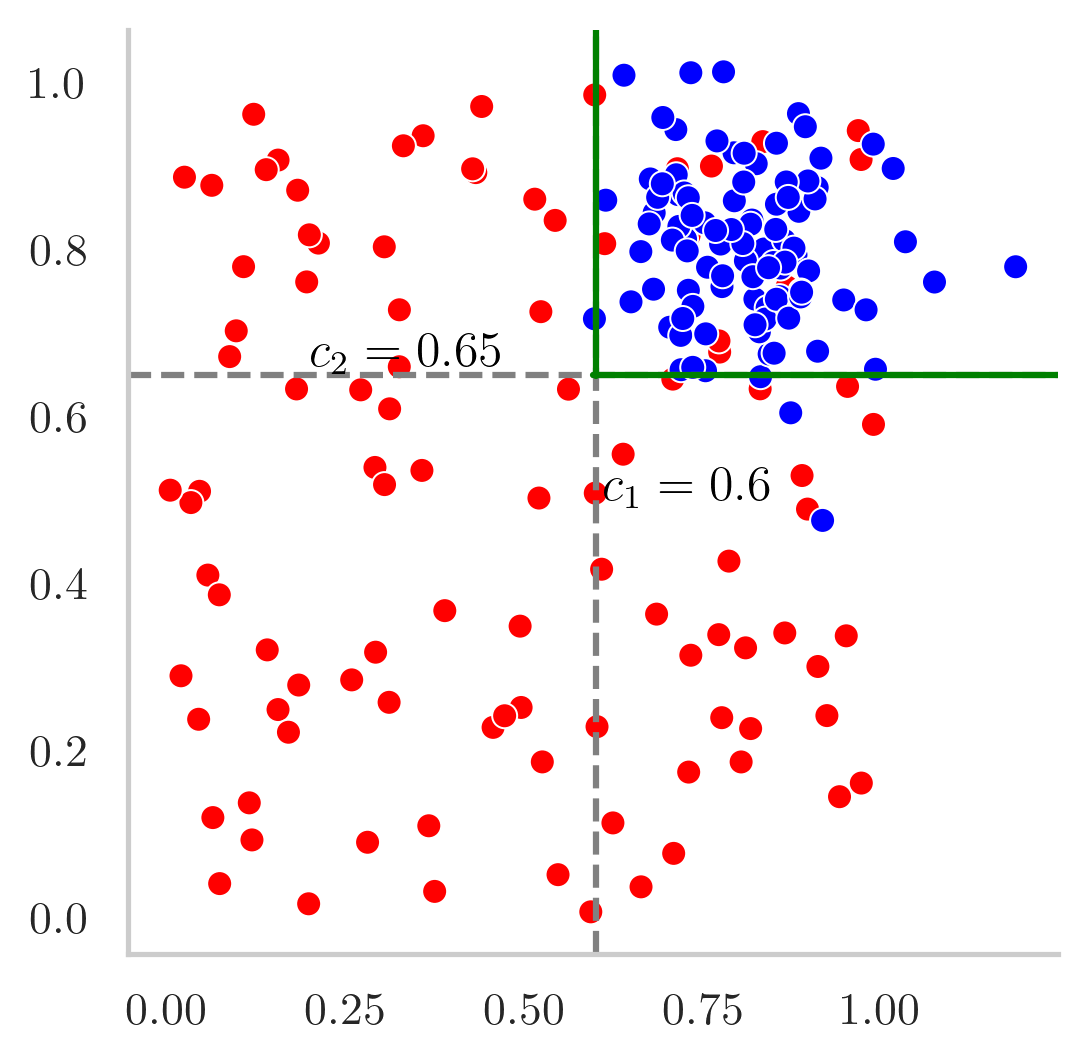
\includegraphics[width=\textwidth]{Images/ML/scatterPlot.png}
      \end{minipage}
\end{figure}
    
Finding the optimal set of partitions of a dataset is an NP-complete problem and therefore intractable for large datasets. To build a tree, a greedy approach must be adopted - meaning using a heuristic approach to find a satsifying solutions, e.g., successively choosing the most optimal step at each stage with no guarantee to find a global optimum instead of a local one. The chosen split is selected based on a defined \textit{cost} function by Equation \ref{eq:DTcost}.

\begin{equation}\label{eq:DTcost}
    (j^*, t^*) = \arg\min_{j\in \{1, ..., D\},\, t \in T_j} \min \left(\text{cost} (\{x_i, y_i : x_{ij} \leq t\}) + \text{cost}(\{x_i, y_i : x_j > t\}) \right)
\end{equation}
where $T_j$ is the set of possible thresholds, $x_j$, $y_j$ are the features and label (or regressive objective). For categorical variable, the inequality $x_j >< t$ would be typically converted in a value equality $x_j == t$. The \textit{cost} function will depend on the objective of the tree, with the regression case typically using the error function \[cost(D) : \sum_{i\in D}(y_i - \bar{y})^2,\] and for a classification the loss would be one of the following:
\begin{itemize}
    \item \textbf{Missclassification rate:} $\frac{1}{|D|} \sum_{i \in D} \mathbb{I}(y_i \neq \hat{y})$, where $D$ is the data in the leaf of the tree and $\mathbb{I}$ is the identity function: $\mathbb{I}(x) = 1$ if $x$ is True, else $0$. 
    \item \textbf{Statistical entropy:} defining the class-condition probability as $\pi_c = \frac{1}{|D|} \sum_{i \in D} \mathbb{I}((y_i) \neq c)$, the entropy over the ($C$) classes is defined in Equation \ref{eq:statEntropy:}
    \begin{equation}\label{eq:statEntropy}
        H(\vec{\pi}) = - \sum_{c=1}^C \pi_c \log \pi_c.
    \end{equation}
    \item \textbf{Information Gain:} an equivalent formulation to the entropy, where the gain in information that should be maximised is the relative change in entropy by adding a selection on feature $X_j$ over the current stage: 
    \[ \text{Gain}(X_j < t, Y) = H(Y) - H(Y | X_j < t) \]
    \item \textbf{Gini:} computes and minimises the expected error rate: \[\sum_{c=1}^C \pi_c (1 - \pi_c).\]
\end{itemize}

The pseudocode algorithm to train a \gls{dt} with the update rule of Equation \ref{eq:DTcost} is summarised in Algorithm \ref{ag:DT}. 

\begin{algorithm}
    \caption{Recursive Procedure to Train a Decision Tree \cite{MurphyML}.}
    \begin{algorithmic}
    \Function{fitTree}{node, $D$, depth}
        \State $\text{node.prediction} \gets \text{mean}(\{y_i : i \in $D$\})$ 
        \State $(j^*, t^*, D_L, D_R) \gets \text{split}(D)$
        \If{\text{not worthSplitting}(\text{depth}, \text{cost}, $D_L$, $D_R$)}
            \State \Return node
        \Else
            \State node.left $\gets$ FITTREE(node, $D_L$, depth + 1)
            \State node.right $\gets$ FITTREE(node, $D_R$, depth + 1)
            \State \Return node
        \EndIf
    \EndFunction
    \end{algorithmic}
    \label{ag:DT}
\end{algorithm}

\gls{dt} can overfit a dataset: the model may tune itself to specific features of the training set that are not generalisable to any set samples from the true original distribution. Regularisation serves as an important step to avoid this often unwanted behaviour. For trees, a natural procedure to avoid overtraining is to interrupt the growth of the tree when it is no longer worth doing so - a criterion that is hard to decide \textit{a priori} - or to \textit{prune} the tree -removong nodes or branches that contribute little to the overall performance. A simpler way to regularise the performance by reducing the variance of the estimate of the model is to train several trees with different subsets of the data chosen randomly with replacement and aggregate the results into a single prediction, for example for regression by taking the average over each base learners: \[ y(x) = \frac{1}{N_l} \sum_{i=1}^{N_l} y_i(x),\] for $N_l$ base learner making prediction $y_i(x)$ given the input features $x$ or by majority voting for the case of classification. This statistical technique of using ensemble of predictors is refered to as \textit{bagging}. To further decorrelate the performance of the different predictors, these can be reduced to a subset of the input features and training points, thereby forming a \textit{random forest}.

\subsection{Boosted Decision Trees}
Another extension to the simple decision trees is to introduce the concept of \textit{boosting}, a method called Boosted Decision Trees (BDT) and, importantly in particle physics, \gls{mva}. Boosting is a greedy algorithm leveraging a weak learner or predictor (e.g., a \gls{dt}) and applying it sequentially to weighted versions of the data, with a larger weight given to missclassified / miss-regressed datapoints. This method is hugely popular in data science, having earned the title \textit{``best off-the-shelf classifier in the world''} \cite{baggingML}. Two particularly useful approaches are adaptive boosting (AdaBoost) \cite{Adaboost} and gradient boosting \cite{gradientBoosting}, both combining an ensemble of $L$ weak learners $f_i$ ($i = 1, ..., L$) into a strong learner \[F(x) = \sum_{i=1}^L f_i(x).\] For the following discussion, the model is built using a training dataset $ \{(x_1, y_1), ..., (x_N, y_N)\}$ with input vectors $x_i \in \{\mathbb{R} \otimes \mathbb{D}\}^d$ of $d$ features that are real or discrete ($\mathbb{D}$) and $y \in \mathbb{R}^d$ is a $d$-dimension real vector that serves as output to be predicted by the model.

\subsubsection{AdaBoost}
AdaBoost combines the $L$ weak learners $h_i$ with adaptive weights $\alpha_i$ to improve the ensemble performance as \[\hat{f}(x) = \sum_{i=1}^L \alpha_i h_i(x),\] where $\hat{f}$ is the boosted model, and the successive boosting stages $f_T = \sum_{i=1}^{T \leq L} \alpha_i h_i(x)$ define stronger and stronger boosted variants of the model. At each iteration $m$ of the training process ($m = 1, ..., L$), a weight $w_i^m$ is assigned to each training sample (indexed by $i$) proportional to the current error or loss: $L(y_i, f_{t-1}(x_i))$. The error in AdaBoost is the exponential loss on the datapoints of Equation \ref{eq:adaboosterror}:

\begin{equation}\label{eq:adaboosterror}
    L(y, f_m(x)) = \sum_{i=1}^N \exp\left(-y_i f_m(x_i)\right) = \sum_{i=1}^N \exp\left(-y_i (f_{m-1}(x_i) + \alpha_m h_m(x_i))\right),
\end{equation}
where the typical case for AdaBoost is binary classification with $y_i \in {-1, 1}$ but the algorithm can be generalised to other cases. Equation \ref{eq:adaboosterror} can be re-expressed to highlight the weight $w_{i,m}$ applied to each datapoint $(x_i, y_i)$ at step $m$ as : \[\sum_{i=1}^N w_{i,m} \exp\left(-\alpha_m y_i h_m(x_i)\right),\] where $w_{i,m} = \exp\left(-y_i f_{m-1}(x_i)\right)$. The weak learner at step $m$ is applied to the weighted version of the dataset with weights $w_{i,m}$ and combined with the strong learners with optimal weight $\alpha_m$ found by minimising the error to be \[\alpha_m = \frac{1}{2} \log \frac{1 - \epsilon_m}{\epsilon_m},\] where $\epsilon_m$ is the ratio of miss-classified weights: $\epsilon_m = \sum_i w_{i,m} \mathbb{I}(y_i \neq h_m(x_i)) / \sum_i w_{i,m}$. The overall update rule is then given by Equation \ref{eq:updateOverall}:
\begin{equation}\label{eq:updateOverall}
    f_m(x) = f_{m-1}(x) + \alpha_m h_m(x),
\end{equation}
combining the new weak learners $h_m$ with optimal weight $\alpha_m$ to the current stronge learner. The AdaBoost algorithm is summarised in Algorithm \ref{algo:adaboost}.

\begin{algorithm}
    \caption{Adaboost for Binary Classification with Exponential Loss \cite{MurphyML}}
    \label{algo:adaboost}
    \begin{algorithmic}
    \State Initialise weights: $w_i = \frac{1}{N}$, where $N$ is the number of samples.
    \For{$m = 1$ to $M$}
        \State Fit a classifier $h_m(x)$ to the training set using weights $w$.
        \State Compute $\epsilon_m = \sum_i w_{i,m} \mathbb{I}(y_i \neq h_m(x_i)) / \sum_i w_{i,m}$.
        \State Compute $\alpha_m = \log\left(\frac{1 - \epsilon_m}{\epsilon_m}\right)$.
        \State Update weights: $w_i \leftarrow w_i \, \exp(\alpha_m \cdot \mathbb{I}(y_i \neq h_m(x_i)))$.
    \EndFor
    \State \Return $f(x) = \text{sgn}\left(\sum_{m=1}^M \alpha_m h_m(x)\right)$
    \end{algorithmic}
\end{algorithm}

\subsubsection{Gradient boosting}
Gradient boosting is a generic approach which, contrary to AdaBoost, does not require a specific derivation for each loss function. The objective is to minimise the empirical risk, the expected value of the loss function $L$ on the training set as shown in Equation \ref{eq:empRisk} 
\begin{equation}\label{eq:empRisk}
    \hat{f}  = \arg \min_f \mathbb{E}_{x,y} L(y, f(x))
\end{equation}
where $f(x) = (f(x_1), ..., f(x_N))$ is the output of the learner on the training set. As the name suggests, the approach leverages gradient descent to find the optimal $\hat{f}$. At step $m$, the gradient of the loss $L(f)$ is evaluated at $f = f_{m-1}$ as \[ g_{i,m} = \left[ \frac{\partial  L(y_i, f(x_i))}{\partial f(x_i)} \right]_{f= f_{m-1}}, \] which is then used to update the learner with a step \[ f_m = f_{m-1} - \alpha_m g_{m}\] of step-length $\alpha_m$ chosen to minimise the residual loss $L(y, f_{m-1} - \alpha_m g_{m})$. \\
For the specific case of gradient boosted decision trees, at step $m$ a decision tree $h_m(x)$ is fitted to the pseudo-residuals. This \gls{dt} $h_m$ at step $m$ defines $J_m$ disjoint regions through its leaves with predictions $b_{jm}$ in each $j = 1, ... J_m$ region: \[ h_m(x) = \sum_{j=1}^{J_m} b_{jm} \textbf{1}_{R_{jm}}(x),\] where $\textbf{1}_{R_{jm}}(x)$ is the indicator function - equals to 1 when $x \in R_{jm}$ and 0 otherwise. The update to the model is chosen so that: \[f_m(x) = f_{m-1} + \alpha_m h_m(x),\] with $\alpha_m$ selected by minimising the empirical risk of the updated model: \[ \alpha_m = \arg \min_{\alpha} \sum_{i=1}^N L(y_i, f_{m-1}(x_i) + \alpha h_m(x_i)).\]

\begin{algorithm}
    \caption{Gradient Boosting \cite{MurphyML}}
    \label{algo:gradient_boosting}
    \begin{algorithmic}
    \State Initialise $f_0(x) = \arg\min_\alpha \,\sum_{i=1}^N L(y_i, h(x_i; \alpha))$
    \For{$m = 1$ to $M$}
        \State Compute the gradient residual $\forall i$: $g_{i,m} = -\left[\frac{\partial L(y_i, f(x_i))}{\partial f(x_i)}\right]_{f(x_i) = f_{m-1}(x_i)}$
        \State Train weak learner $h_m$ on the dataset $\{(x_i, r_{i,m})\}_{i=1}^N$
        \State Compute $\alpha_m$ by minimising $\sum_{i=1}^N(g_{i,m} - \alpha_m h_m(x_i))$
        \State Update $f_m(x) = f_{m-1}(x) + \nu \alpha_m h_m(x)$
    \EndFor
    \State \Return $f(x) = f_M(x)$
    \end{algorithmic}
\end{algorithm}

The full algorithm for Gradient Boosting is presented in Algorithm \ref{algo:gradient_boosting}, where the update rule is added a \textit{learning rate} hyperparameter $\nu$ to introduce regularisation and reduce the risk of overfitting. By keeping $0 < \nu \leq 1$, it limits the ability of the model to fully adapt to the training error, thereby improving generalisation. The price is a slower updating of the model and therefore a more demanding computational complexity. Further regularising techniques are bootstrap aggregation - training each weak learner on a random subset of the data -, limiting the number of leaves, or more generally penalising model of larger complexity - removing branches that do not reduce the loss by a minimal amount. \\

\gls{bdt} resist better to overtraining thanks to the regularisation effect of boosting and the different techniques described in this section. Unfortuntaly, an undiserable feature of boosting is the loss of direct interpretability behind decision but this is more than met by an appreciable \textit{boost} in performance of the underlying model.\\

\textbf{Pros:}
\begin{itemize}
    \item \textit{High Accuracy:} \gls{bdt} easily achieve high accuracy in both classification and regression tasks, making them suitable for a wide range of applications.
    \item \textit{Ensemble Learning:} The boosting technique combines multiple weak learners to create a strong learner, improving overall model performance.
    \item \textit{Robustness to Overfitting:} Boosting helps mitigate overfitting, enhancing the model's generalisation to unseen data.
    \item \textit{Feature Importance:} \gls{bdt} provide a measure of feature importance, aiding in feature selection and interpretability of the model.
    \item \textit{Non-linearity Handling:} They can capture non-linear relationships in the data, offering more flexibility than linear models.
    \item \textit{Adaptability to Different Distributions:} Boosting algorithms, such as AdaBoost and Gradient Boosting, can adapt well to different types of data distributions.
\end{itemize}

\textbf{Cons:}
\begin{itemize}
    \item \textit{Sensitivity to Noisy Data:} \gls{bdt} can be sensitive to noisy data and outliers, potentially leading to overfitting.
    \item \textit{Computational Complexity:} Training multiple weak learners sequentially can be computationally expensive, especially for large datasets or deep tree structures.
    \item \textit{Parameter Tuning:} It is crucial to fine-tune the hyperparameters, such as learning rate and tree depth, for optimal performance.
    \item \textit{Black Box Nature:} The ensemble nature of boosted decision trees make them somewhat of a "black box,"  sacrifing interpretability for the sake of performance.
\end{itemize}

\subsection{Artificial Neurons}
The Artificial Neuron, also called the \textit{perceptron} by its inventor Frank Rosenblatt in his seminal 1958 paper \cite{rosenblatt1958perceptron}, is the logical gate that underpins most \gls{dl} models: for example, a \gls{mlp} - also called a \gls{dnn} - is just a stacking of layers of artificial neurons. Inspired by biological principles, the perceptron, as represented in figure \ref{fig:annModel} takes multiple outputs and gives as output 1 if the combination of inputs exceeds a certain specific threshold, otherwise giving 0. This combination accepts weights to scale the input which, remarkably, can be adjusted during a training phase if the output of the perceptron is incorrect. Artificial neurons are a direct generalisation of this very principle, with the output no longer being thresholded but applied a chosen function after being added a learnable bias term $b$. 

\begin{figure}[h!]
    \center
    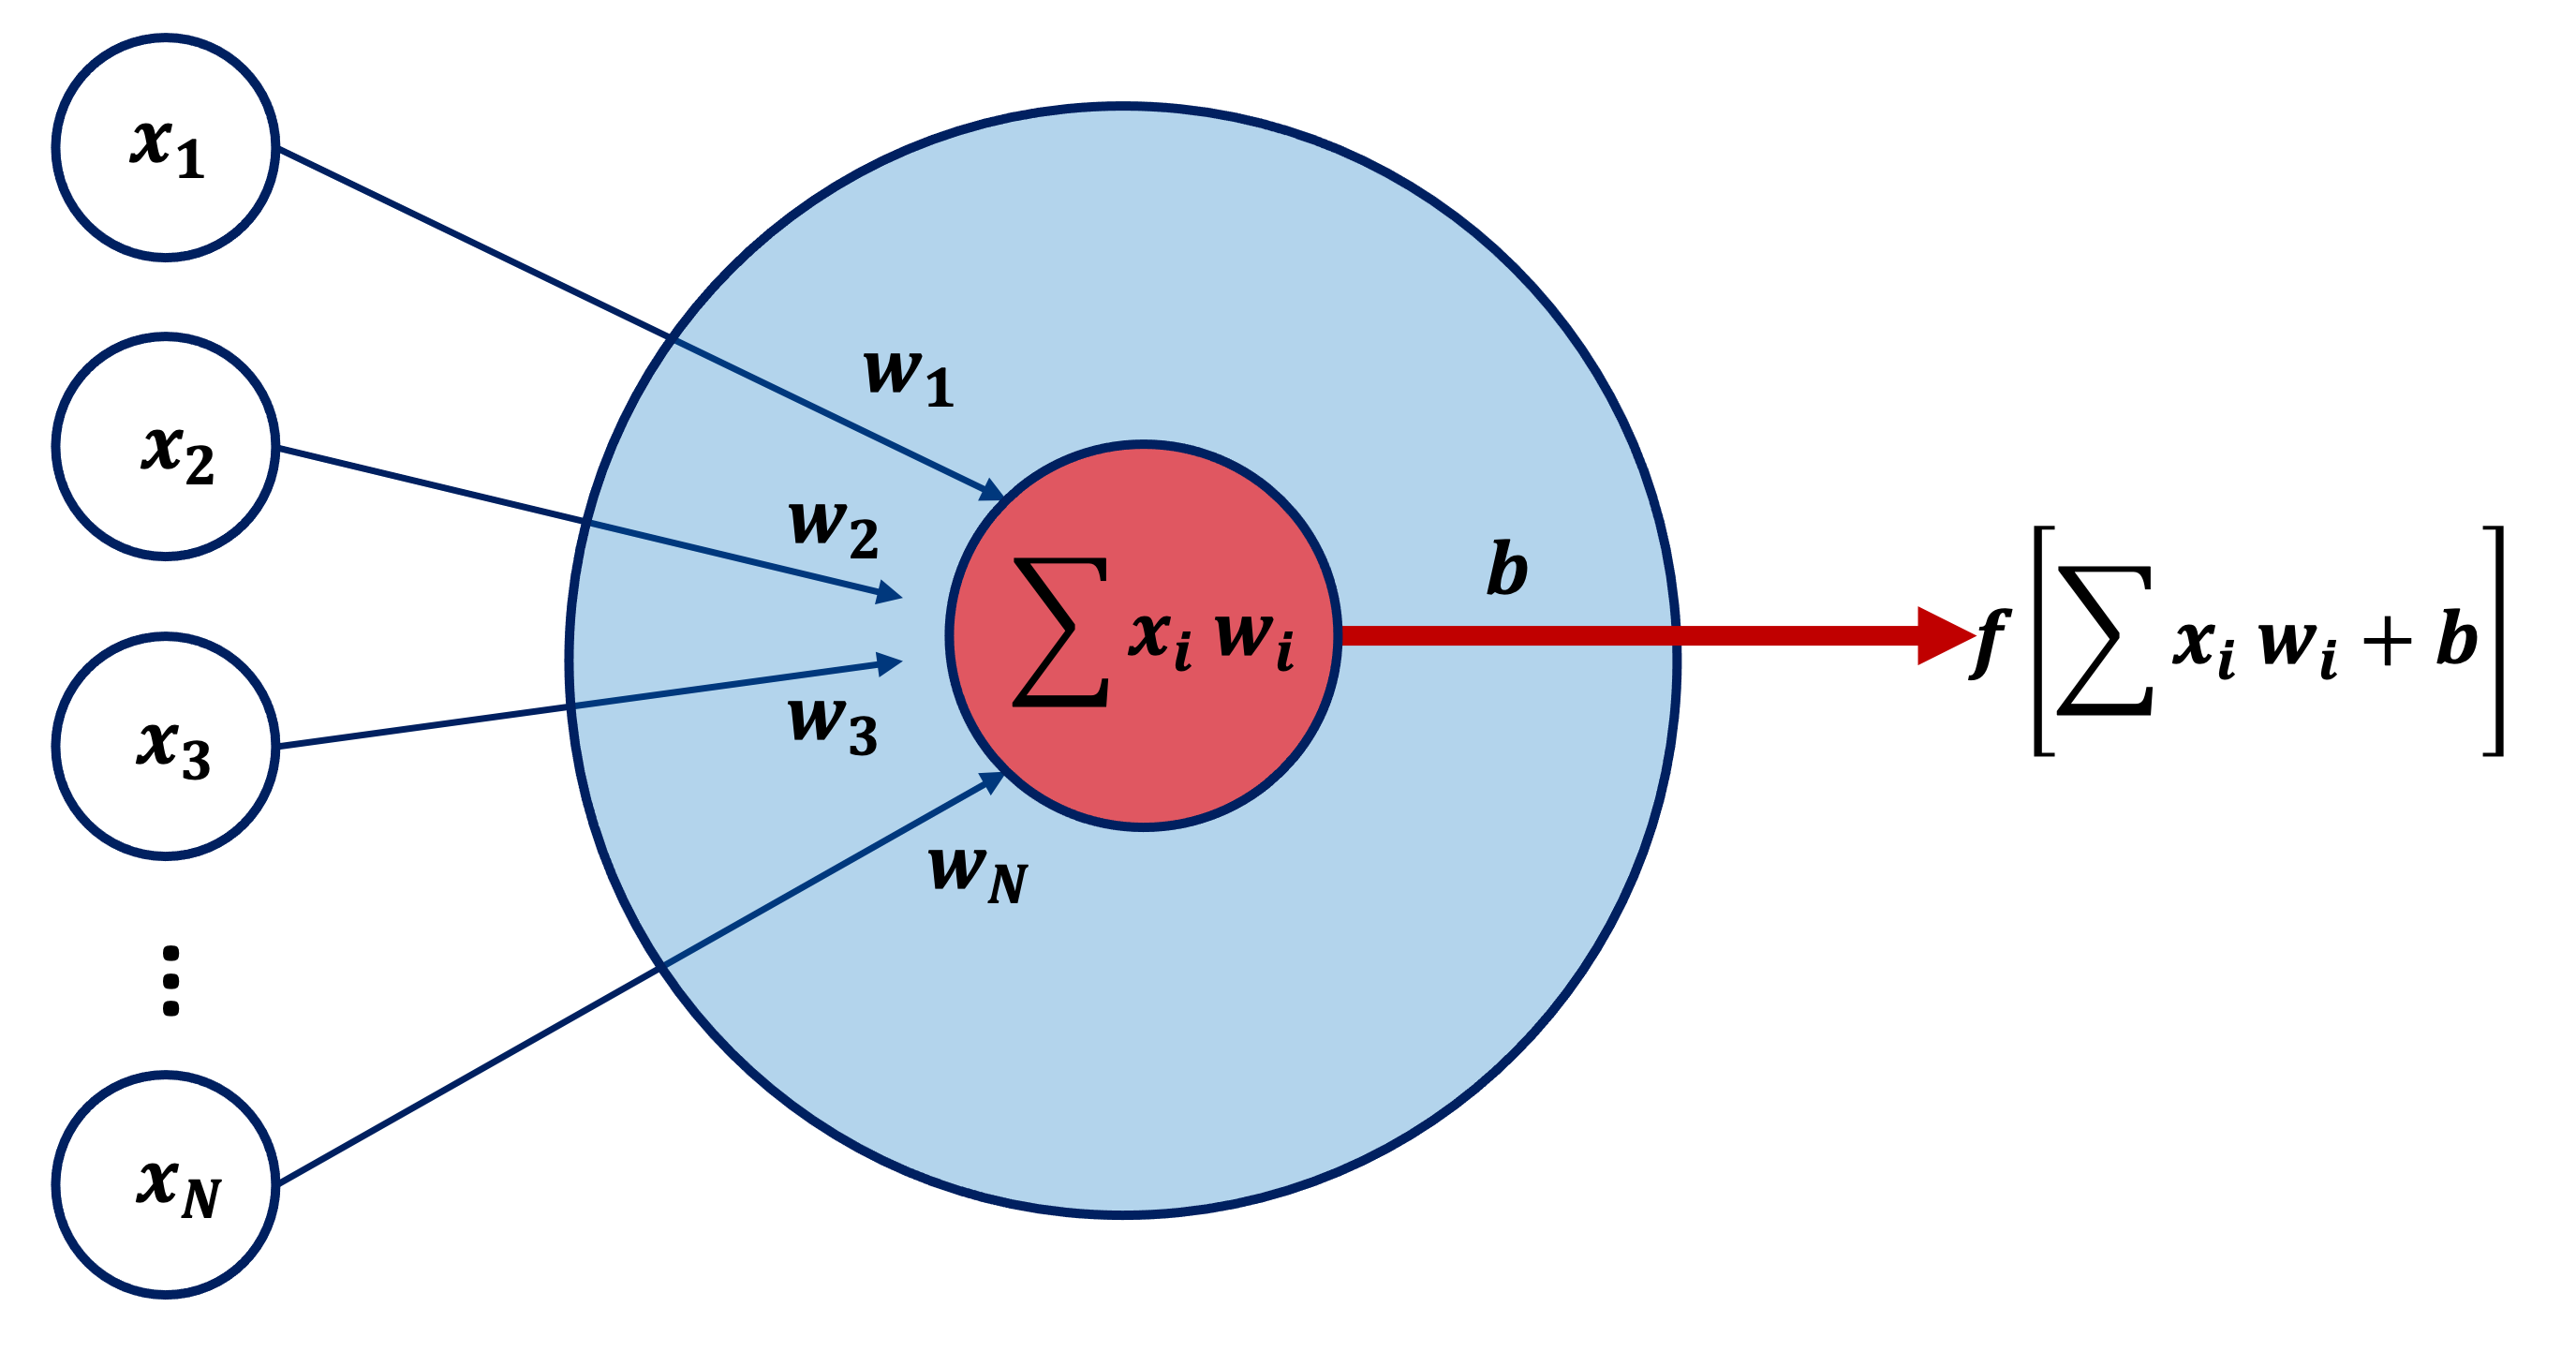
\includegraphics[scale=0.4]{Images/ML/ann.png}
    \caption{Schematics of a perceptron or an artifical neuron: the inputs $x_i$ ($i= 1, ..., N$) is multiplied by learnable weights $w_i$, summed and added a bias $b$ before being passed to an output function $f$.} 
    \label{fig:annModel}
\end{figure}

In this thesis, a \textit{perceptron} shall refer to a single artificial neuron, which is equivalent to a logistic regression model. The interest of the artificial neuron steams from a significant theoretical result: stacks of artificial neurons are \textit{universal function approximator} \cite{universalFuncApproxNN,HORNIK1989359}, as is shown in the next section on deep neural network. This theoretical result is built on a mathematically advantageous function choice for $f$: the sigmoid $\sigma$, defined in equation \ref{eq:sigmoid} and shown in Figure \ref{fig:sigmoid:}
\begin{equation}\label{eq:sigmoid}
    \sigma(x) = \frac{1}{1 + e^{-x}.}
\end{equation}

\begin{wrapfigure}{R}{0.5\textwidth}
    \begin{center}
        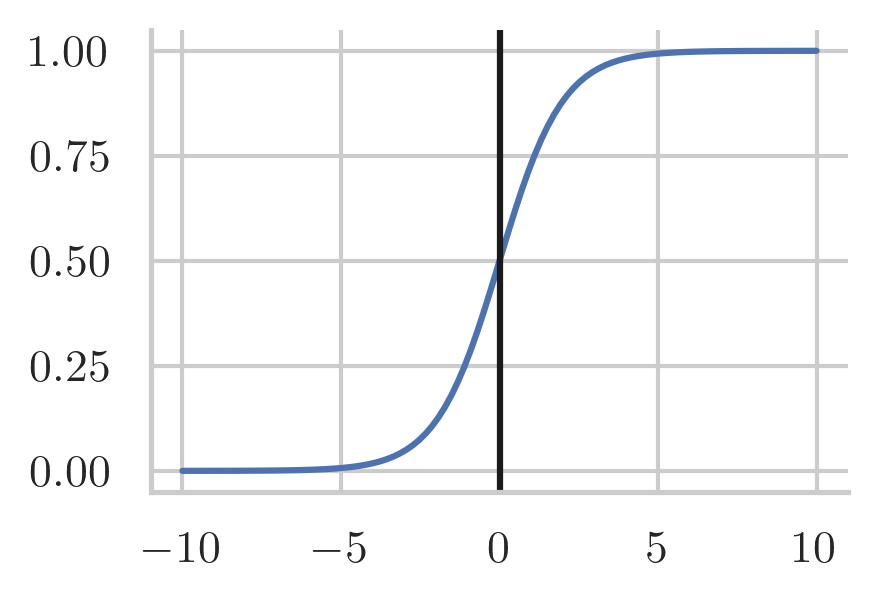
\includegraphics[width=0.45\textwidth]{Images/ML/sigmoid.png}
        \caption{The sigmoid function $\sigma(x)$.} 
        \label{fig:sigmoid}
    \end{center}
\end{wrapfigure}

Thanks to its property to map the range of real numbers to the [0, 1] range, this activation function is often used for numerical stability and to map to probabilities. The nice mathematical property of the sigmoid that is particularly relevant for \gls{dl} is its simple to compute derivative: \[\sigma^\prime(x) = \sigma(x) (1- \sigma(x)).\]

The power of artificial neuron comes from their ability to be efficiently combined. For an input $x \in \mathbb{R}^d$, each neuron individually applies an affine transformation $W_i^T x + b_i$, where $W_i \in \mathbb{R}^d,\,b_i \in \mathbb{R}$ are the weights and bias of the neuron $i$, that is passed through an activation function $f$ for a total output of a single neuron $f(W_i^T x + b_i)$.

\subsection{Deep Neural Networks}
A \gls{dnn}, also called \gls{mlp}, \gls{ann}, \gls{nn}, or feed-forward neural network, is made by stacking along depth layers of artificial neurons - the width - as shown in Figure \ref{fig:neuralnet}. Layers of artificial neurons that are placed between the input and output layers are said to be \textit{hidden layers}. The particular design of this architecture is that layers of neurons connect to neurons of the next layers only, defining a feed-forward computation graph from input $x$ to output $y$. Mathematically, a single layers at depth $i$ with $m$ units given as input the previous layer of dim $n$ at depth $i-1$ computes the  transformation of Equation \ref{eq:feedforward:}
\begin{equation}\label{eq:feedforward}
    a^i = f^i\left({W^i}^T a^{i-1} + b_i\right),
\end{equation}
where $W^i \in \mathbb{R}^{m \times n}$ is the matrix of weight of layer $i$ - one row per unit of layer $i$, one column per unit of layer $i-1$, $b_i \in \mathbb{R}^m$ is the vector of bias, one per unit of layer $i$, and $f^i$ is the activation function of layer $i$. Note that strictly speaking the activation could be different for the units of the layer but is often unique per layer to accelerate matrix computations.

\begin{figure}[h!]
    \center
    \begin{minipage}[l]{0.38\textwidth}
        \caption{A deep neural network with $d$ layers of width $m$, $l$ ...$k$. Each artificial neuron, represented by a ball of darkening blue along depth, computes a linear transformation of the input of the layer followed by an activation function. The input of the \gls{dnn} is $x$ and the output is $y$} 
    \label{fig:neuralnet}
      \end{minipage}
      \begin{minipage}[c]{0.6\textwidth}
        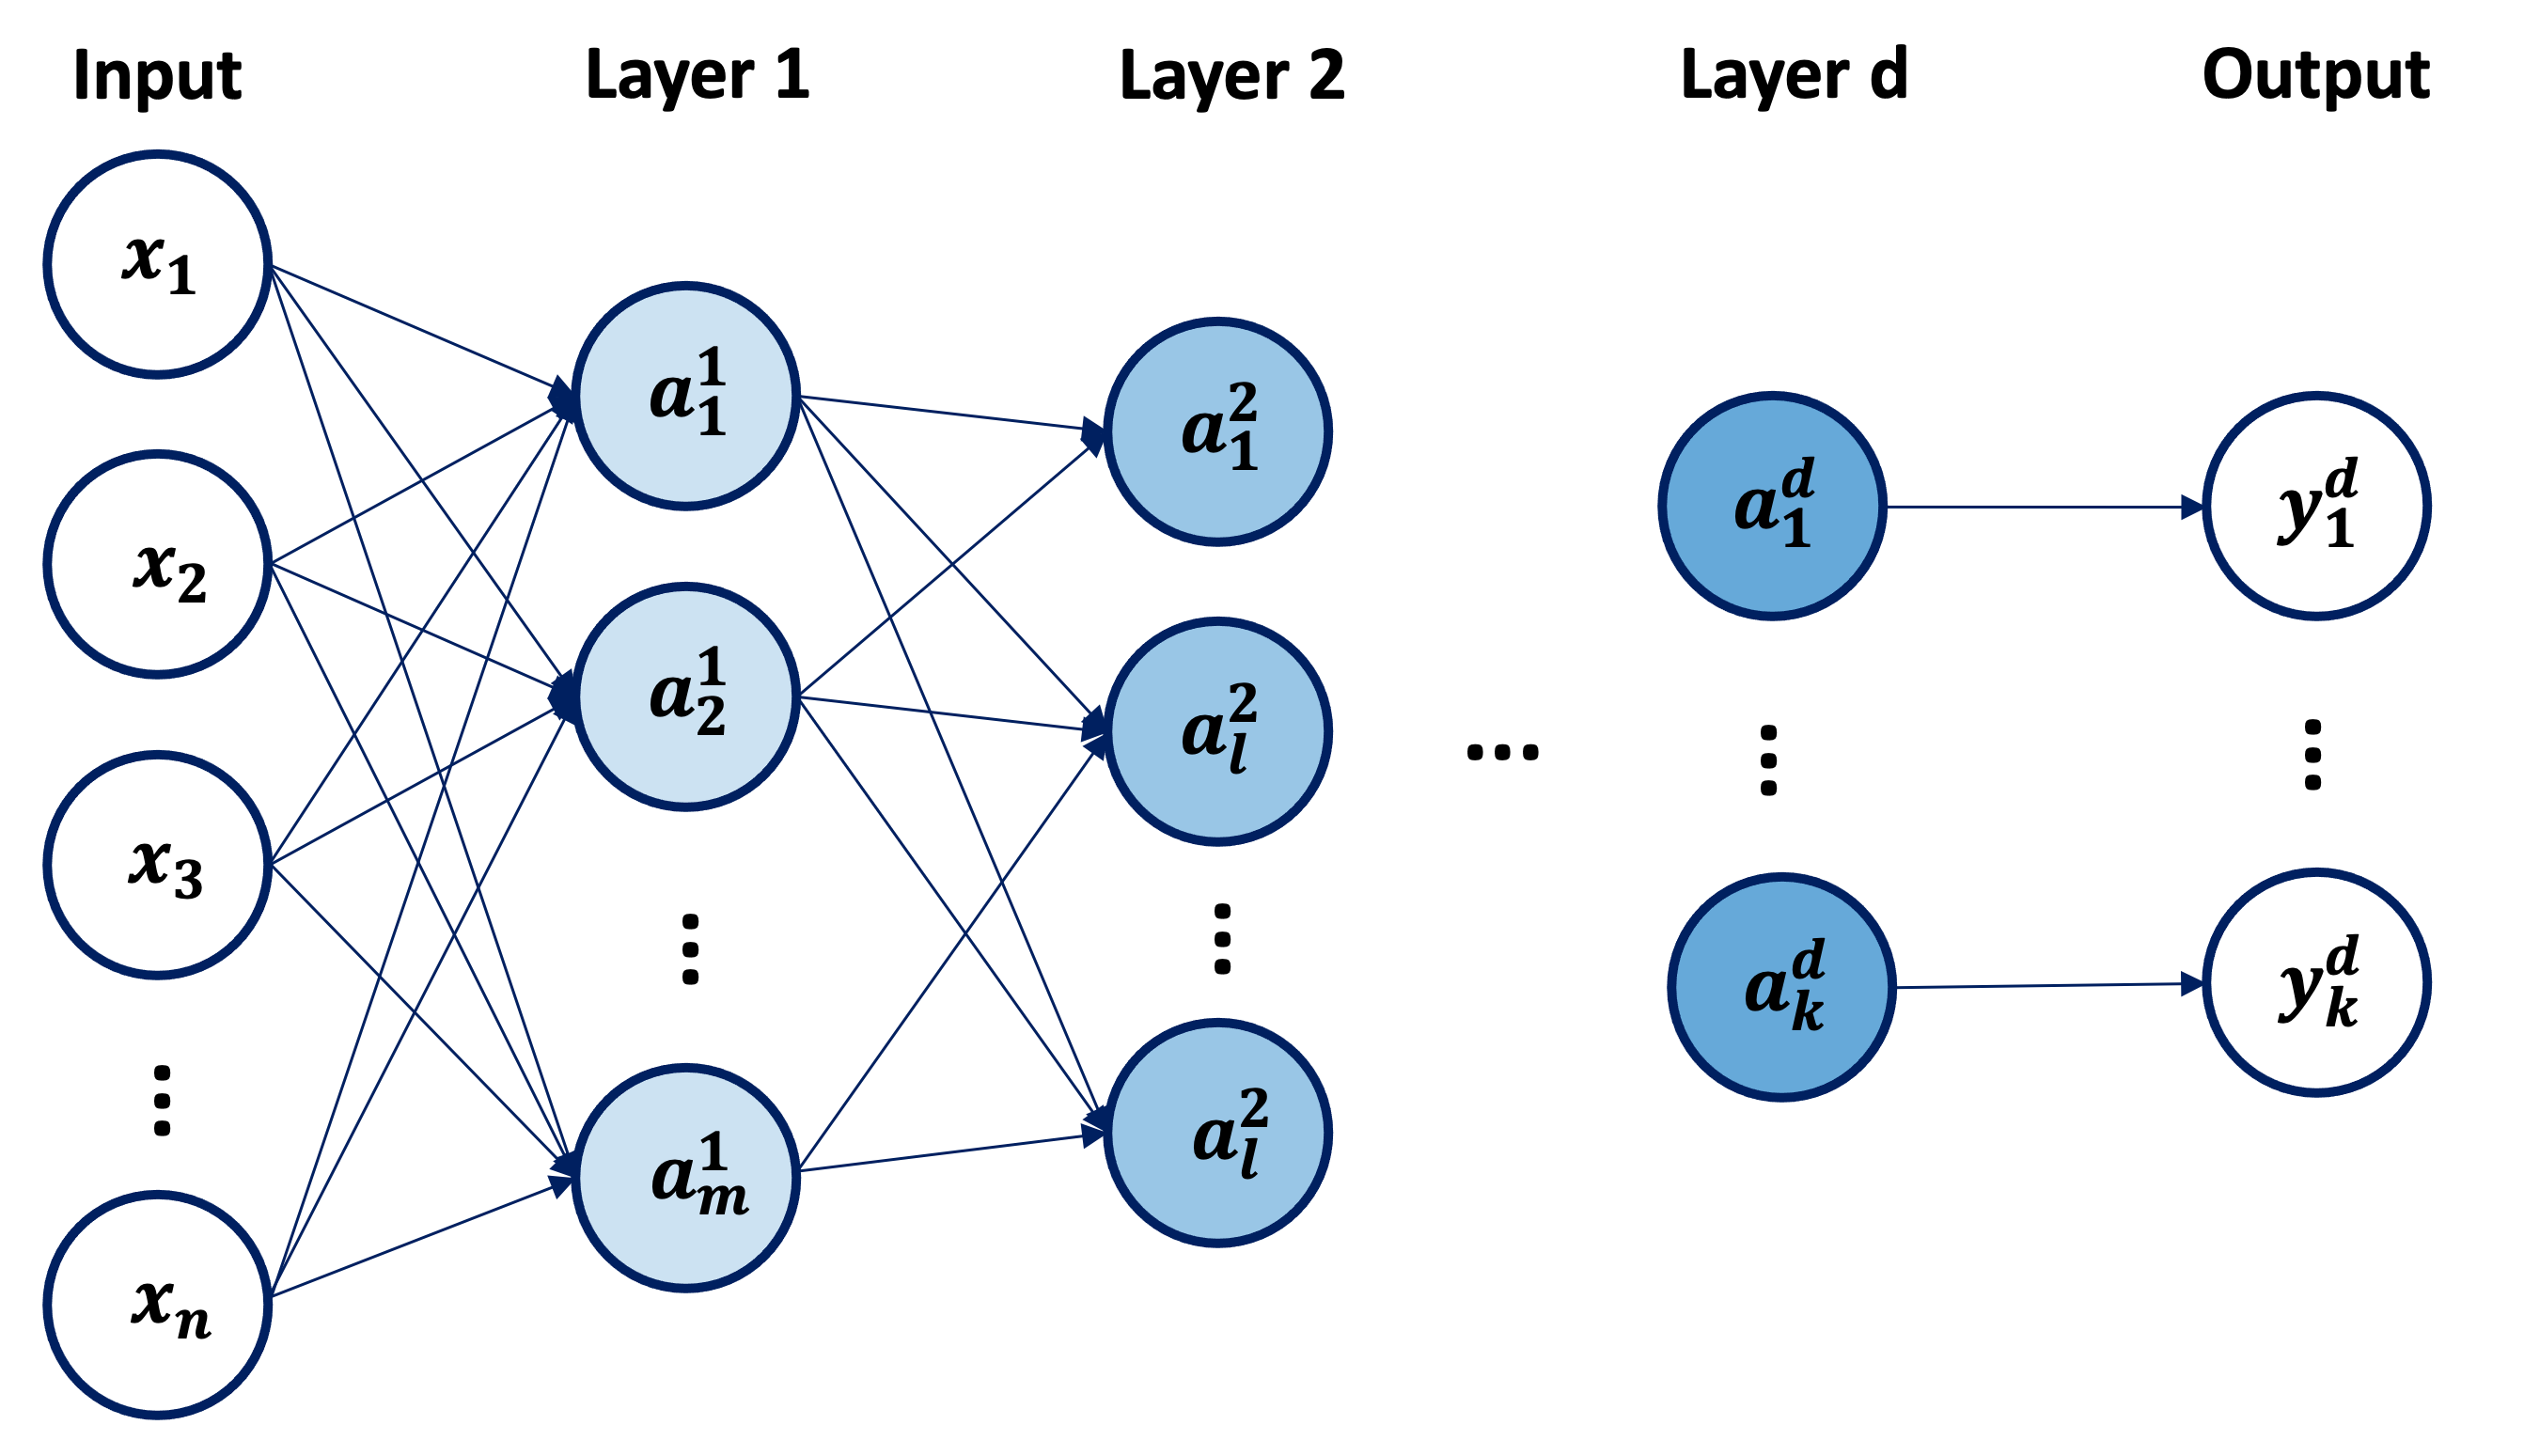
\includegraphics[width=\textwidth]{Images/ML/neuralnet.png}
      \end{minipage}
\end{figure}

Neural networks implement a system computing combination of Equation \ref{eq:feedforward}. A powerful theoretical motivation for neural networks stems from the fact they are Universal Function Approximator. This theorem, or rather family of theorem depending on the type of activation $f$ considered, proves that neural network built with appropriate functions are able to approximate most well-behaving functions - sufficiently smooth. It states \cite{universalFuncApproxNN,HORNIK1989359:} 
\paragraph{Theorem:} \textit{Let $C([0, 1]^n)$ denote the set of all continuous function $[0, 1]^n \rightarrow \mathbb{R}$ and $\sigma$ be any sigmoidal activation function. Then the finite sum $f(x) = \sum_{i=1}^N \alpha_i \sigma(w_i^T x + b_i)$ is dence in $C([0, 1]^n)$. In other words, given any $f \in C([0, 1]^n)$ and $\epsilon > 0$, $\exists$ a sum $G(x)$ of the above form for which: \[ G(x) - f(x) < \epsilon \quad \forall x \in [0, 1]^n.\]}

This essentially states that any function defined over the $n$-dimensional unite hypercube $[0, 1]^n$ can be approximated by an arbitrarily wide neural network. This result only requires $\sigma$ to be discriminatory in the sense:
\begin{equation}
    \sigma(x) \rightarrow
    \begin{cases}
        1 \text{ if } x \rightarrow \inf  \\
        0 \text{ if } x \rightarrow -\inf
    \end{cases}
\end{equation}
which is satisfied by the sigmoid function. Interestingly, similar theorems were derived for other important function commonly used in \gls{dl}, for example for ReLu in \cite{universApproximator-Relu}. Many flavours of \gls{dnn} exist with varying function being used. An important theoretical result is the requirement for the output function applied to the artificial neuron to possess some degree of \textit{non-linearity} - otherwise the model collapses to a large linear regression. Such functions, when applied to the output of an artificial neuron, are said to \textit{activate} it and is hence called \textit{activation functions}. The most popular such functions, shown in Figure \ref{fig:commonAct}, are:
\begin{itemize}
    \item The sigmoid function of Equation \ref{eq:sigmoid}
    \item The hyperbolic tangent function $\tanh = \frac{e^x - e^{-x}}{e^x + e^{-x}}$
    \item The \gls{relu} function of Equation \ref{eq:relu}
    \begin{equation}\label{eq:relu}
        \text{ReLu}(x) = \text{max}(0, x)
    \end{equation}
    \item The Exponential Linear Unit (ELU) function, shown in Equation \ref{eq:elu}, generalises the ReLu in the negative domain while keeping the saturation property, which introduces a hyperparameter $\alpha > 0$:
    \begin{equation}\label{eq:elu}
        \text{Elu}(x) = 
        \begin{cases}
            x \quad \text{ if } x >= 0 \\
            \alpha (e^x - 1)  \quad  \text{ otherwise}
        \end{cases}
    \end{equation}
    \item The softmax function. For an $x \in \mathbb{R}^n$, the softmax return a vector softmax$(x) = [..., \frac{e^{x_i}}{Z}, ...]$ (for $i= 1, ..., N$), where $Z = \sum_i e^{x_i}$. For a 2-dimensional $x$, the softmax is equivalent to the sigmoid function. In $n$-dimension, it maps each entry of $x$ to the range $[0, 1]$ and guarantees $\sum_i softmax(x)_i = 1$. The softmax is therefore  helpful to define probability distributions over multidimensional outputs.
\end{itemize}

\begin{wrapfigure}{R}{0.5\textwidth}
    \begin{center}
        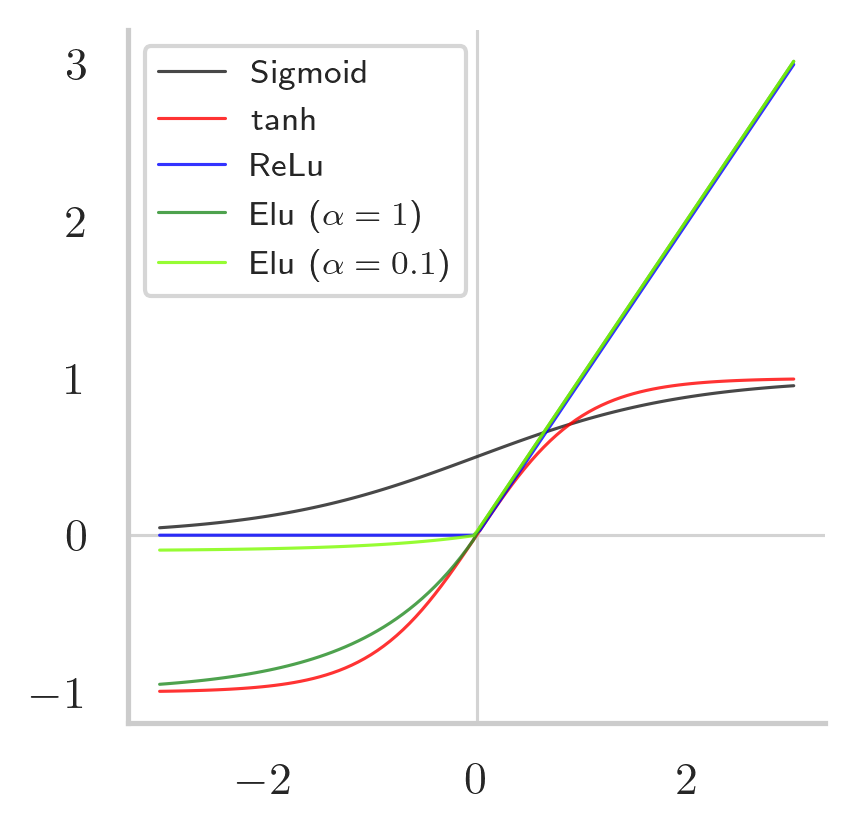
\includegraphics[width=0.45\textwidth]{Images/ML/activations.png}
        \caption{The most common non-linear activations used in deep learning.} 
        \label{fig:commonAct}
    \end{center}
\end{wrapfigure}
Of course, many more functions have been defined in the field of \gls{ai}, yet none seem to offer a clear advantage over the ones listed here. The sigmoid is no-longer the choice of reference, as it quickly saturates - meaning its gradient for large positive and negative values vanishes. The hyperbolic tangent $\tanh$ offers steeper gradients thanks to its [-1, 1] range and is often the activation of choice for autoregressive architecture, such as the \gls{rnn}. The \gls{relu} functions is the most widely used activation function as its derivative is extremelly efficient to compute and does not suffer from vanishing gradient for positive values. Its fixed 0-value for negative input is a double edge sword: on one side, it helps the network regularises itself by deactivating neurons, on the other it could let some neurons being stuck in \textit{off}-mode if their weights are such that the pre-activation value is always negative for the input data. For this reason, it is important to correctly initialises the weights of a \gls{dnn}. An easy work around this limitation is the Elu activation, which introduces some leakage in the negative value - as controlled by a parameter $\alpha$.\\
While the Universal Function Approximator theorem gives a powerful endorsment of \gls{dl} networks, it does not state how one can be obtained to fit a specific function. The task of choising the right architecture (depth and width) and the correct weights and bias must be approximated by a learning strategy updating the weights and biases to reduce the error between the output and a given target. Many models are Universal Function Approximator and what sets appart \gls{dl}-like model that are built on artificial neurons is the simplicity of the procedure to update the weights: thanks to their nice computational structure, under a reasonable choice of activation function for each layer, the network is \textit{differentiable}. This means a gradient can be computed on a function measuring the difference between the target $y$ and the output $\hat{y}$ - often called a loss function when it should be minimised or a reward function when it is to be maximised - and \textit{back-propagated} along each neuron of each layer to give a local update to be applied to each individual weight and biases. The recent rise of \gls{dl} in \gls{ai} can be traced back to improvement in making this backpropagation of the gradient and public libraries, such as PyTorch \cite{pytorch} and TensorFlow \cite{tensorflow2015-whitepaper}, implementing efficient algorithm to perform this essential step. \\
One of the main difficulty in training a neural network is the non-convexity of the loss function as a function of the model parameters. The large number of parameters typically implemented by neural networks further require large dataset to correctly assign them to values without suffering from overtraining - the property to only correctly describe the data of the training set without being able to generalise the performance. These can be summarised into two difficulties encountered by neural networks: the non-convexity of the objective function meaning saddle points and local minima are possible - and typically abundant - and the computational complexity due to the large number of parameters. To circumvent these, the \textit{backpropagation} algorithm of Algorithm \ref{ag:backpropagation} is used \cite{backprop}.

\begin{algorithm}
    \caption{Backpropagation Algorithm}
    \begin{algorithmic}
    \Function{Update}{$x$, $y$, $N$, $\mathcal{L}$}
        \State Forward step: propagate input $x$ through network $N$ to get prediction $\hat{y}$
        \State Loss: compute the loss or reward of $N$: $\mathcal{L}(y, \hat{y})$
        \State Back-propagate gradients:
        \While{Layer not-updated}
            \State Take right-most layer not computed yet 
            \State Take output of layer to the right 
            \State Using the chain-rule of calculus, propagate gradient of next layer to that of current layer
            \State Store the gradient at the layer
            \State remove current layer from consideration
        \EndWhile
    \EndFunction
    \end{algorithmic}
    \label{ag:backpropagation}
\end{algorithm}

In summary, the backpropagation algorithm serves as an effective way to compute \[ \frac{\partial\mathcal{L}(\theta)}{\partial\theta} = \sum_{i=1}^N \frac{\partial l(\theta)}{\partial\theta},\] 
where $\theta$ encapsulates all parameters of the model and there are $N$ datapoints, with a per datapoint loss of $l$. 
The backpropagation algorithm starts with a forward pass through the network: \[ x \xrightarrow{\times W^1 + b^1} z^1 \xrightarrow{f^1()} a^1 \xrightarrow{\times W^2 + b^2} z^2 \xrightarrow{f^2()} a^2 \xrightarrow{\times W^3 + b^3} ... \xrightarrow{\times W^d + b^d} a^d = \hat{y},\] the loss is then computed $\mathcal{L}(y, \hat{y} | W^1, b^1, W^2, b^2, ..., W^d, b^d)$ before computing the gradient of each layer by starting from the right:\[\text{grad}_{W^d, b^d} = \nabla_{W^d, b^d} \mathcal{L} \rightarrow \text{grad}_{W^{d-1}, b^{d-1}} = \nabla_{W^{d-1}, b^{d-1}} \text{grad}_{W^d, b^d} \rightarrow ... \rightarrow \nabla_{W^{1}, b^1} \text{grad}_{W^2}, \]
where the operation $\text{grad}_{W^{d-1}, b^{d-1}} = \nabla_{W^{d-1}} \text{grad}_{W^d}$ implies a use of the chain rule to obtain the local gradient, based on information already obtained. In the context of \gls{dl}, the chain rule of multivariate calculus offers a transformation:
\begin{equation}
    \frac{\partial h}{\partial x} = \frac{\partial h}{\partial z}\frac{\partial z}{\partial x},
\end{equation}
for a function $h: \mathbb{R}^n \rightarrow \mathbb{R}^m$, $f: \mathbb{R}^n \rightarrow \mathbb{R}^k$, $g: \mathbb{R}^k \rightarrow \mathbb{R}^m$, and $h = g \circ f$ with $x \in \mathbb{R}^n$ and $z = f(x)$. Two types of updates are necessary: 
\begin{itemize}
    \item For a layer $l$: \[\frac{\partial l}{\partial z^l} = \frac{\partial l}{\partial a^l} . \frac{\partial a^l}{\partial z^l}\]
    \item For a layer $l$ having access to previous layer $l+1$ $(\frac{\partial l}{\partial z^{l+1}})$: \[\frac{\partial l}{\partial z^l} = \frac{\partial l}{\partial z^{l+1}} \frac{\partial z^{l+1}}{\partial z^l} = \frac{\partial l}{\partial z^{l+1}} \frac{\partial z^{l+1}}{\partial a^l} \frac{\partial a^l}{\partial z^l}, \] but since $z^{l+1} = W^{l+1}a^l + b^{l+1}$, this reduces to:\[\frac{\partial l}{\partial z^l} = \frac{\partial l}{\partial z^{l+1}} W^{l+1} \frac{\partial a^l}{\partial z^l}, \]

    \item Combining the two above, we can compute $\frac{\partial l}{\partial z^l}$ for each layer in backward order. One thus now requires the derivative with respect to the per-layer weights: \[\frac{\partial l}{\partial W^l} = (a^{l-1} \frac{\partial l}{\partial z^l})^T,\] 
    
    for the weight matrix - an outer product between a row vector $\frac{\partial l}{\partial z^l}$ and a column vector $a^{l-1}$. For the bias: \[\frac{\partial l}{\partial b^l} = \frac{\partial l}{\partial z^l},\] the result is directly obtained from the row vector. 
\end{itemize}

Once all the gradients are locally available, the next step is to update all the parameters to reduce the loss by taking a step in the direction opposed to the gradient, giving the largest reduction in loss. For example for a specific parameter $w_{ij}$ at training step $t+1$:
\begin{equation}\label{eq:gradientdescent}
    w^{T=t+1}_{ij} \leftarrow w^{T=t}_{ij} - lr \times \text{grad}\left[w^{T=t}_{ij}\right],
\end{equation}
where the \textit{learning rate} $lr$ controls how large a step is taken in the opposite direction of the gradient. Since the gradient of the earlier layers will be derived from the gradient of later layers, it is important for the gradients to respect some numerical stability to avoid the risk of vanishing gradient ($\rightarrow$ 0) or exploiding gradients ($\rightarrow \inf$). This requires some care in the architecture choice and might justify the use of a specific activation function over another. Note that strictly speaking, the activation function needs not be a continuous differentiable function ($C^1$), as the existence of a right or left differential continuity ($C^0$) are sufficient. \\
Concerning the loss function $\mathcal{L}$, there is a lot of freedom in how to set it up - although it should be differentiable - and some typical choices are:
\begin{itemize}
    \item The cross-entropy loss function - also called the logistic loss - is based on the notion of entropy, as defined in Equation \ref{eq:statEntropy}, and is often used to assign probabilities in a classification with $c$ classes: \[ -y_i \log\hat{y}_i,\] where $y_i$ is the real label of the datapoint and $\hat{y} \in [0, 1]^C$ is the model prediction, respecting $\sum_i \hat{y}_i = 1$. Given the requirements on the output, it is typically combined with a softmax. 
    \item the Mean Squared Error (MSE) \[\frac{1}{N}\sum_i^N (y_i - \hat{y}_i)^2,\] 
    \item the Mean Absolute Error (MAE) \[\frac{1}{N}\sum_i^N |y_i - \hat{y}_i|,\]
\end{itemize} 
To regularise the model, it is common to add terms to the loss function called \textit{regulariser} in order to restric the model weights to a certain size. This can be achieved by adding to the loss $\mathcal{L}$ an L2-penalty \[\lambda \sum_i w_i^2,\] on the sum of the squared values of the weights, or an L1-penalty \[\lambda \sum_i |w_i|,\] where this last approach using the absolute value has the nice additional feature to make the network sparse - meaning to set un-necessary weights at 0. The amount of regularisation is controlled by the hyperparameter $\lambda$. Further regularisation can be obtained by randomly dropping out some connexions of the network during training, a technique called \textit{dropout} and controled by the dropout probability $p$ to incude an artificial neuron or not.\\
This section introduces deep neural networks, the simplest feed-forward architecture constituted of artificial neurons stacked into layers to generate an output $y$ based on an input $x$. There are many refinements to this base architecture, and some are explored in the next sections. 

\textbf{Pros:}
\begin{itemize}
    \item \textit{Universal Function Approximators:}
    Feedforward networks, particularly deep ones, are known to be universal function approximators. They can approximate any continuous function to arbitrary precision given sufficient hidden units and appropriate activation functions.
    \item \textit{Flexible Architecture:} The architecture of feedforward networks is flexible, allowing for customization in terms of the number of layers, the number of neurons in each layer, and the choice of activation functions. This flexibility makes them suitable for various tasks.
    \item \textit{Feature Learning:} Feedforward networks can automatically learn hierarchical representations of features from the input data. This is beneficial for tasks where the underlying patterns are complex and not easily captured by handcrafted features.
    \item \textit{Non-linearity Handling:} By introducing non-linear activation functions, feedforward networks can capture and model non-linear relationships in data, enabling them to solve more complex problems compared to linear models.
    \item \textit{Availability of Optimisation Techniques:} Various optimisation techniques, such as gradient descent and its variants, are well-suited for training feedforward networks. This makes it possible to efficiently update the network's weights during the training process.
\end{itemize}

\textbf{Cons:}
\begin{itemize}
    \item \textit{Limited Modeling of Sequential Data:} Feedforward networks are not naturally designed for handling sequential data and temporal dependencies. Recurrent Neural Networks (RNNs) or Transformer architectures are often preferred for tasks involving sequential information.
    \item \textit{Fixed Input Size:} Traditional feedforward networks have a fixed input size. While techniques like padding or resizing can be employed, they might not be suitable for handling inputs of varying lengths in tasks like natural language processing.
    \item \textit{Lack of Memory:} Feedforward networks do not have an inherent memory mechanism, which can be a limitation when dealing with tasks requiring the model to retain information over a sequence of inputs.
    \item \textit{Vanishing and Exploding Gradients:} Training deep feedforward networks can be challenging due to the vanishing and exploding gradient problems. Gradients may become too small or too large during backpropagation, leading to difficulties in learning deep representations.
    \item \textit{Need for Sufficient Labeled Data:}Feedforward networks, especially deep ones, often require a large amount of labeled data for effective training. In domains where labeled data is scarce, the performance may be limited.
\end{itemize}

\subsection{Recurrent Neural Networks}\label{sec:RNN}
The first modification to the \gls{dnn} considered in this thesis is the \gls{rnn}. These models were derived to work with sequences, such as occuring in \gls{nlp}. While the architecture is simular to a \gls{dnn}, the change occurs in the way information is passed through the network: \gls{rnn} are autoregressive models. The information flow is bi-directional: the input of a node is consituted of the input and, in addition, the output of the node at a prior timestep. Under certain condition, this cyclical flow can be unfolded into a direct acyclical computational graph that, for a specific amount of timestep, can be approximated by a \gls{dnn}. Figure \ref{fig:rnnNet} presents the structure of an \gls{rnn}-based network as well as its unfolding. The mathematical structures implemented by this architecture is that of Equation \ref{eq:rnnModel:}
\begin{equation}\label{eq:rnnModel}
    y_t = W(h_t) = W(V(x_t) + U(h_{t-1})),
\end{equation}
where $U$, $V$, and $W$ are three potentially different \gls{dnn} mapping taking at timestep $t$ respectively the previous hidden state $h_{t-1}$, the current input $x_t$ and the new hidden state $h_t = V(x_t) + U(h_{t-1})$. The input $x$ is a sequence of $N$ tokens. The initial hidden state $h_0$ is usually initiated from a special mapping from the whole input. An interesting feature of such a network is its ability to build an internal memory of previous inputs to a timestep $T$ thanks to the chain of hidden states $h_{t<T}$. To avoid having gradients of norms too high (exploding gradients) and too low (vanishing gradients), which would not let the model correctly update during gradient descent, the $\tanh$ function is often used as activation in \gls{rnn} thanks to its smooth distribution and limitation to the range $[-1, 1]$. Unfortunately, due to the network relying on the numerical multiplication of many numbers in $[-1, 1]$, the effect of much earlier timestep ($h_{t<<T}$) can be lost when processing later input at $T$, a process described as \textit{memory loss} that is due to vanishing gradients. Thankfully, there are several ways for \gls{rnn} to improve on their limited memory: \gls{lstm} and \gls{gru}.

\begin{figure}[h!]
    \center
    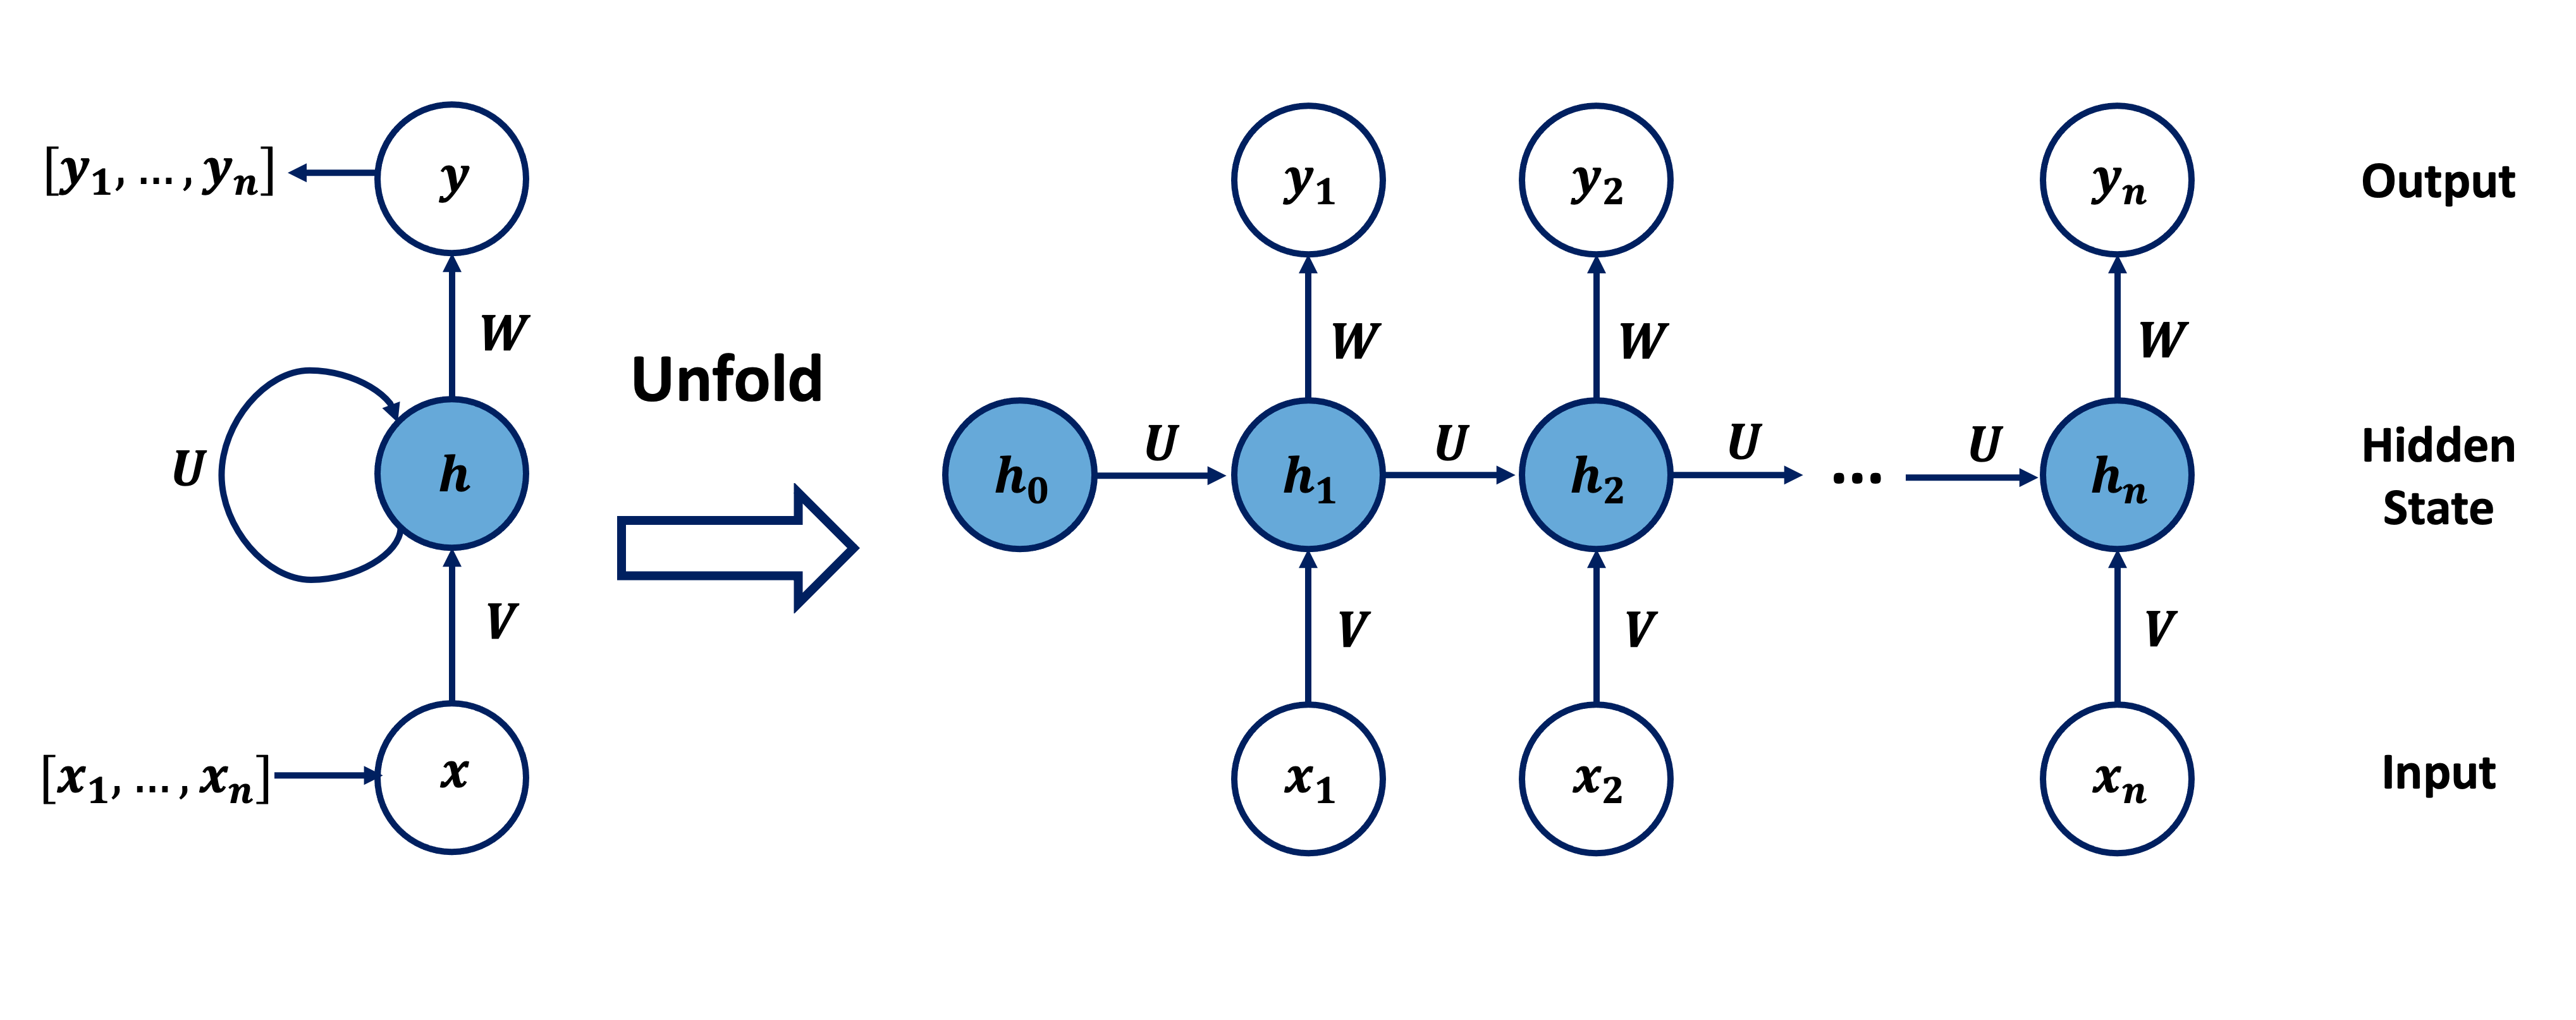
\includegraphics[scale=0.5]{Images/ML/rnn.png}
    \caption{A recurrent neural network, using 3 feed-forward neural networks (DNN) $U$, $V$, $W$, to map the input sequence $x = [x_1, x_2, ..., x_N]$ to the output $y = [y_1, y_2, ..., y_N]$ using the internal hidden state $h^t$ evovling for each timestep $t$.} 
    \label{fig:rnnNet}
\end{figure}

\paragraph{Long-Short Term Memory:} as shown in Figure \ref{fig:lstmCell}, implements a specific architecture to propagate information along the sequence, with the introducion of a new control state $c$ \cite{lstmPaper}. Three gates covering the forget, the input, and the output regulate the flow of information from the cell. In particular, the forget gate decides what information to keep from prior states, by mutliplying these values by a factor 1 and discards the rest through a multiplication by a factor close to 0. The input gate is tasked with creating the new internal state of the cell and what information to store in it.  Finally, the output gate decides which information in the cell should be brought to output. This selectivty of the \gls{lstm} cell to decide what to use from memory, what to keep in memory, and what to output give this architecture a much improved memory for long sequences. 

\begin{figure}[h!]
    \center
    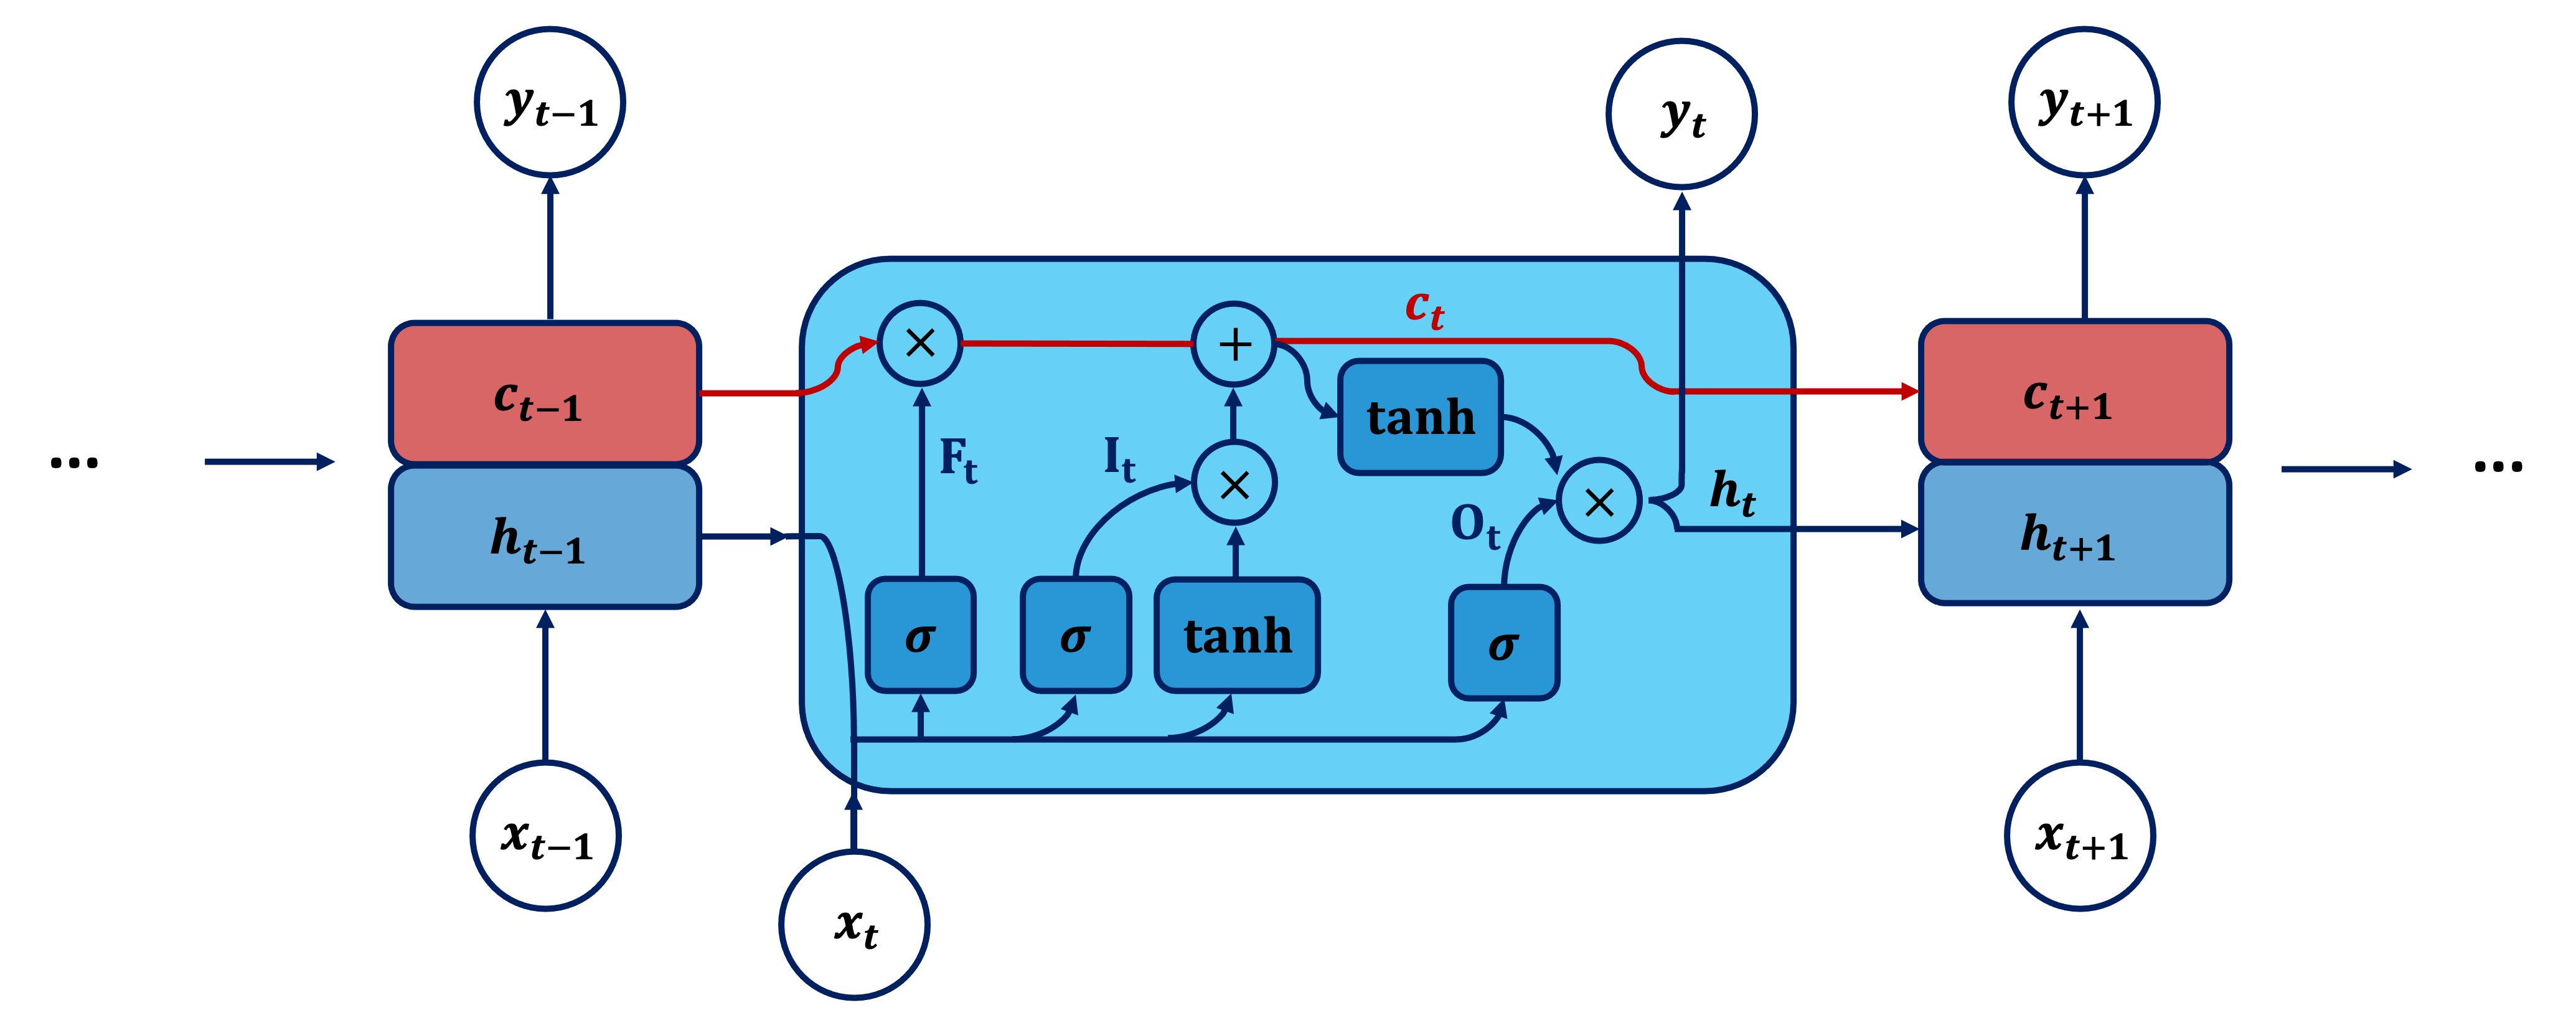
\includegraphics[scale=0.5]{Images/ML/lstm.png}
    \caption{An LSTM cell. Arrows and lines that merge imply concatenation of the inputs, the $\times$, $+$, and tanh are element-wise operation and the $\sigma$ are different layered transformations (1-layer feed-forward network). $F_t$ is the forget gate of the memory cell $c$, $I_t$ the input gate, and $O_t$ the output gate. } 
    \label{fig:lstmCell}
\end{figure}

\paragraph{Gated Recurrent Unit:} another adventageous design to improve the memory of a recurrent-like network without using as many parameters as an \gls{lstm} - there is no output gate and only one internal hidden state $h_t$ is required - is the gated recurrent unit \gls{gru} \cite{gruPaper}. The architecture comes in different version, with the fully gated version presented in Figure \ref{fig:gruCell}, but all only require two gates: the \textit{update gate} $Z_t$ and the \textit{reset gate} $R_t$. The former lets the model decide how much of the past information should be kept and the latter is used to forget past information.

\begin{figure}[h!]
    \center
    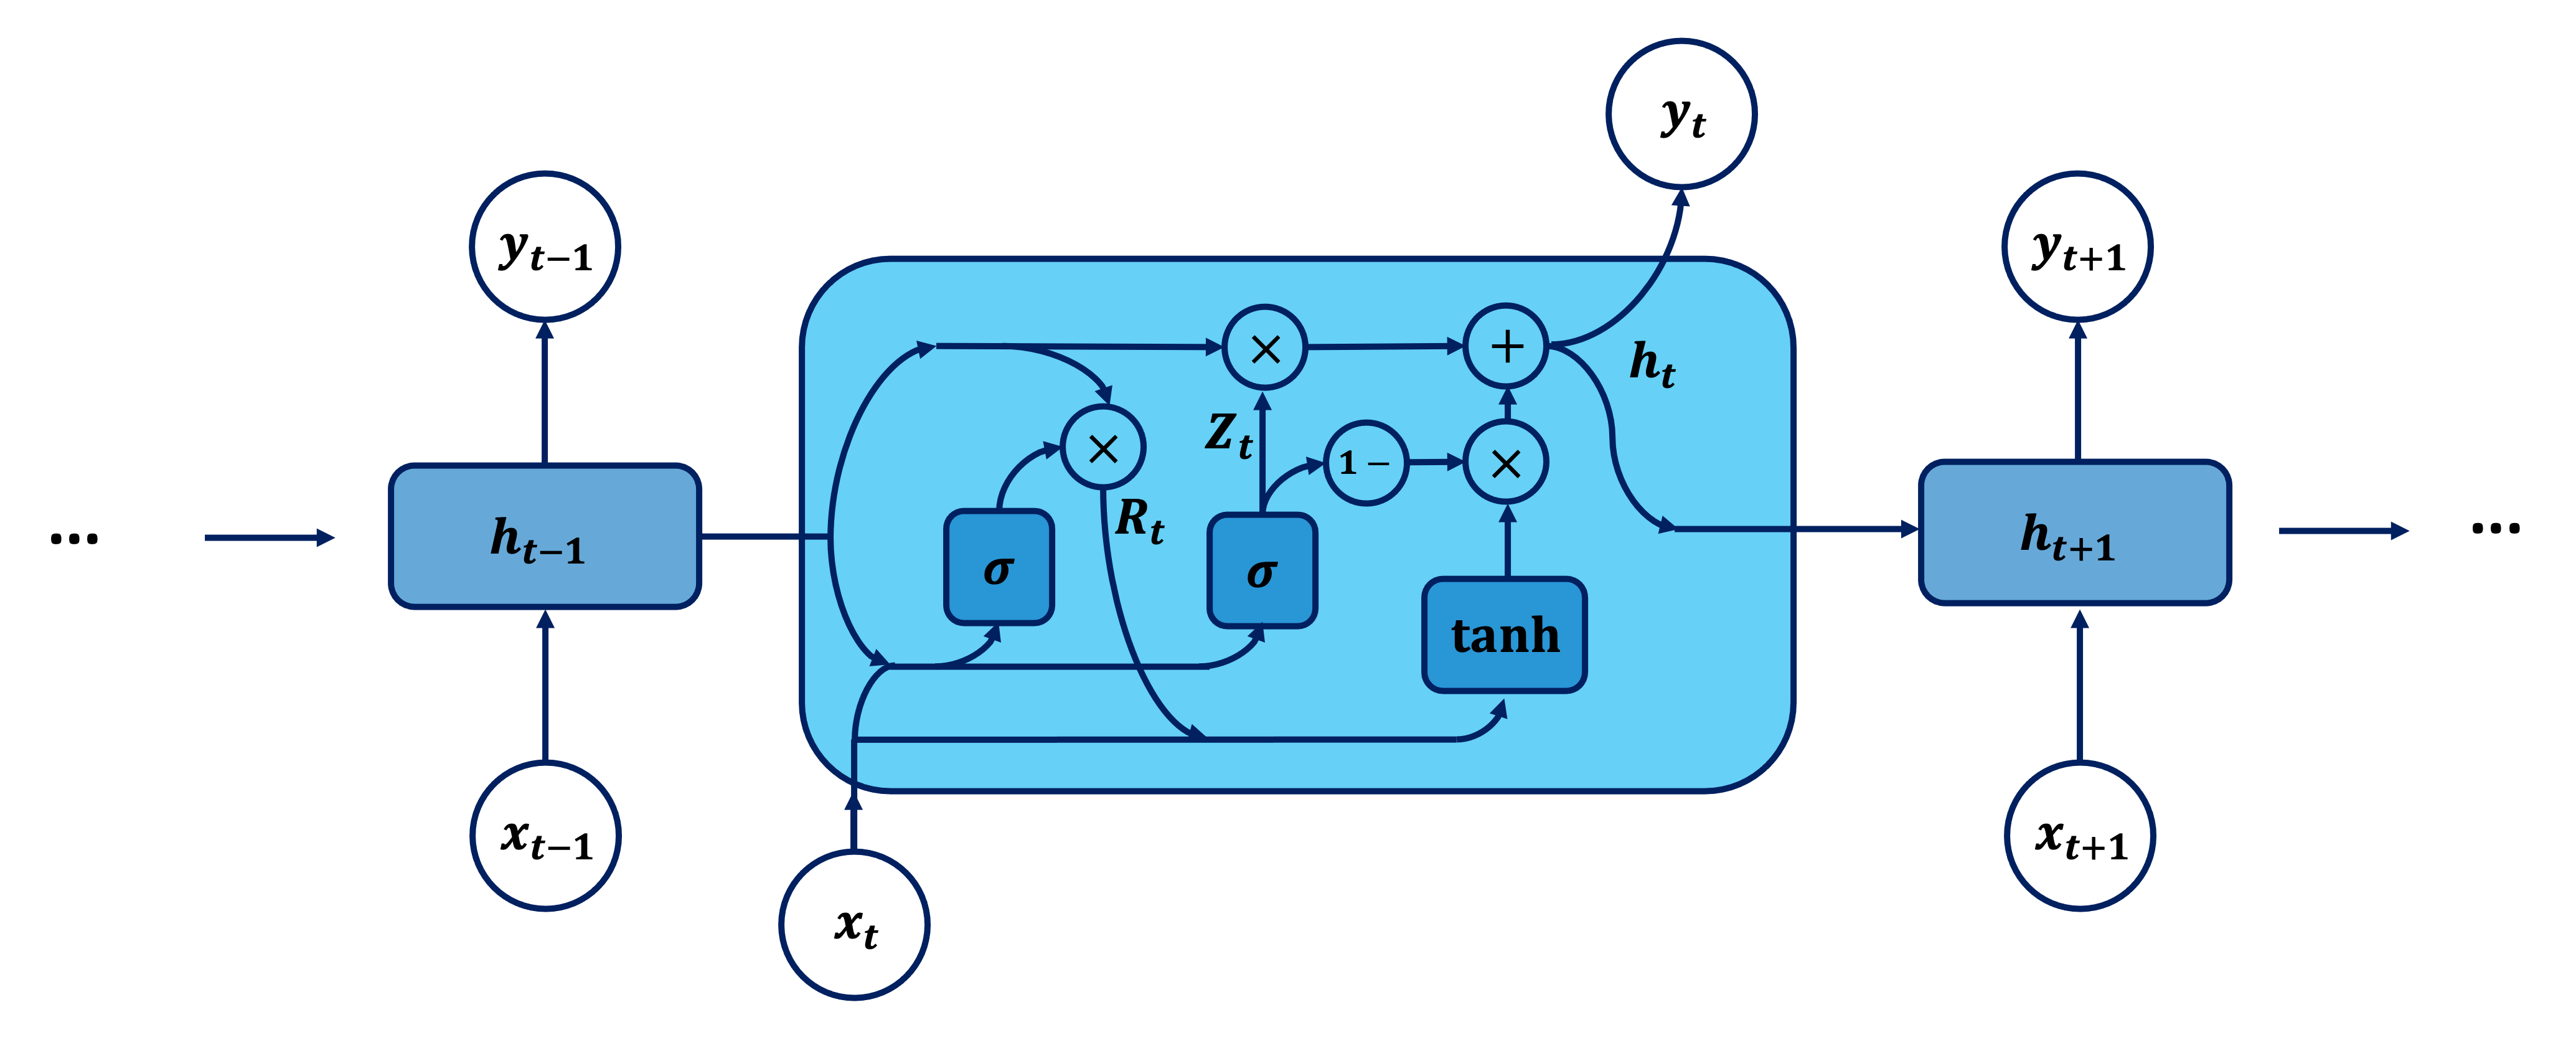
\includegraphics[scale=0.5]{Images/ML/gru.png}
    \caption{A Gated Recurrent Unit cell (fully-gated version). Arrows and lines that merge imply concatenation of the inputs, the $\times$, $+$, tanh, and ``1 - '' are element-wise operation - the last one outputting the vector 1 minus its inputs - and the $\sigma$ are two different layered transformations (1-layer feed-forward network) with sigmoid-like activation function. $Z_t$ is the update gate and $R_t$ the reset gate. } 
    \label{fig:gruCell}
\end{figure}

\gls{rnn}s and their modification have been designed for ordered sequence analysis and have had great results in such settings. An ordered sequence is naturally obtained in language analysis, where a sentence such as \textit{``the boy hit the car''} is meaninguflly different to its permutation \textit{``the car hit the boy''}. The choice to sequentially analyse the tokens of a sequence with memory lets \gls{rnn}s approach problems simularly to a Turing Machine, making them Universal Turing Machine \cite{NEURIPS2021_ef452c63}. A significant drawback however is the impossibility to fully parallelise the analysis of the sequence due to its strict ordering, making \gls{rnn}s expensive models to train even on highly parallelised hardware. The transformer, introduced in section \ref{sec:transformer}, was mainly motivated to fix this latter weakness. \\

\textbf{Pros:}
\begin{itemize}
    \item \textit{Sequential Processing:} \gls{rnn} are designed to handle sequential data, making them suitable for tasks with temporal dependencies.
    \item \textit{Flexibility:} \gls{rnn} can operate on input sequences of variable length.
    \item \textit{Memory:} \gls{rnn} have a memory mechanism that allows them to retain information about previous inputs.
\end{itemize}

\textbf{Cons:}
\begin{itemize}
    \item \textit{Vanishing and Exploding Gradients:} Training deep \gls{rnn} can suffer from vanishing and exploding gradient problems, affecting the learning of long-term dependencies.
    \item \textit{Limited Short-Term Memory:} Traditional \gls{rnn} struggle to capture long-range dependencies due to their limited short-term memory. 
\end{itemize}

These two cons can be mitigated by the use of \gls{lstm} and \gls{gru} architectures. The cost is a more complex architecture, making it harder to train such models and requires more resources. 

\subsection{Convolutional Neural Networks}
Convolutional Neural Networks (\gls{cnn}) \cite{NIPS198953c3bce6, NIPS2012_c399862d} have emerged as a powerful class of deep learning models, particularly effective in computer vision tasks, including image and video analysis. The architecture of \gls{cnn}s is roughly based on human visual processing. It consists of convolutional layers - implementing the fundamental convolution operation-, pooling layers, and feed-forward layers (\gls{dnn}). This architecture, presented in Figure \ref{fig:cnnDesign}, enables \gls{cnn} to automatically learn hierarchical representations of features while respecting properties of image-based data: spaciality (geometrical grounding), locality (neighbourhoods) and spatial symmetry.

\begin{figure}[h!]
    \center
    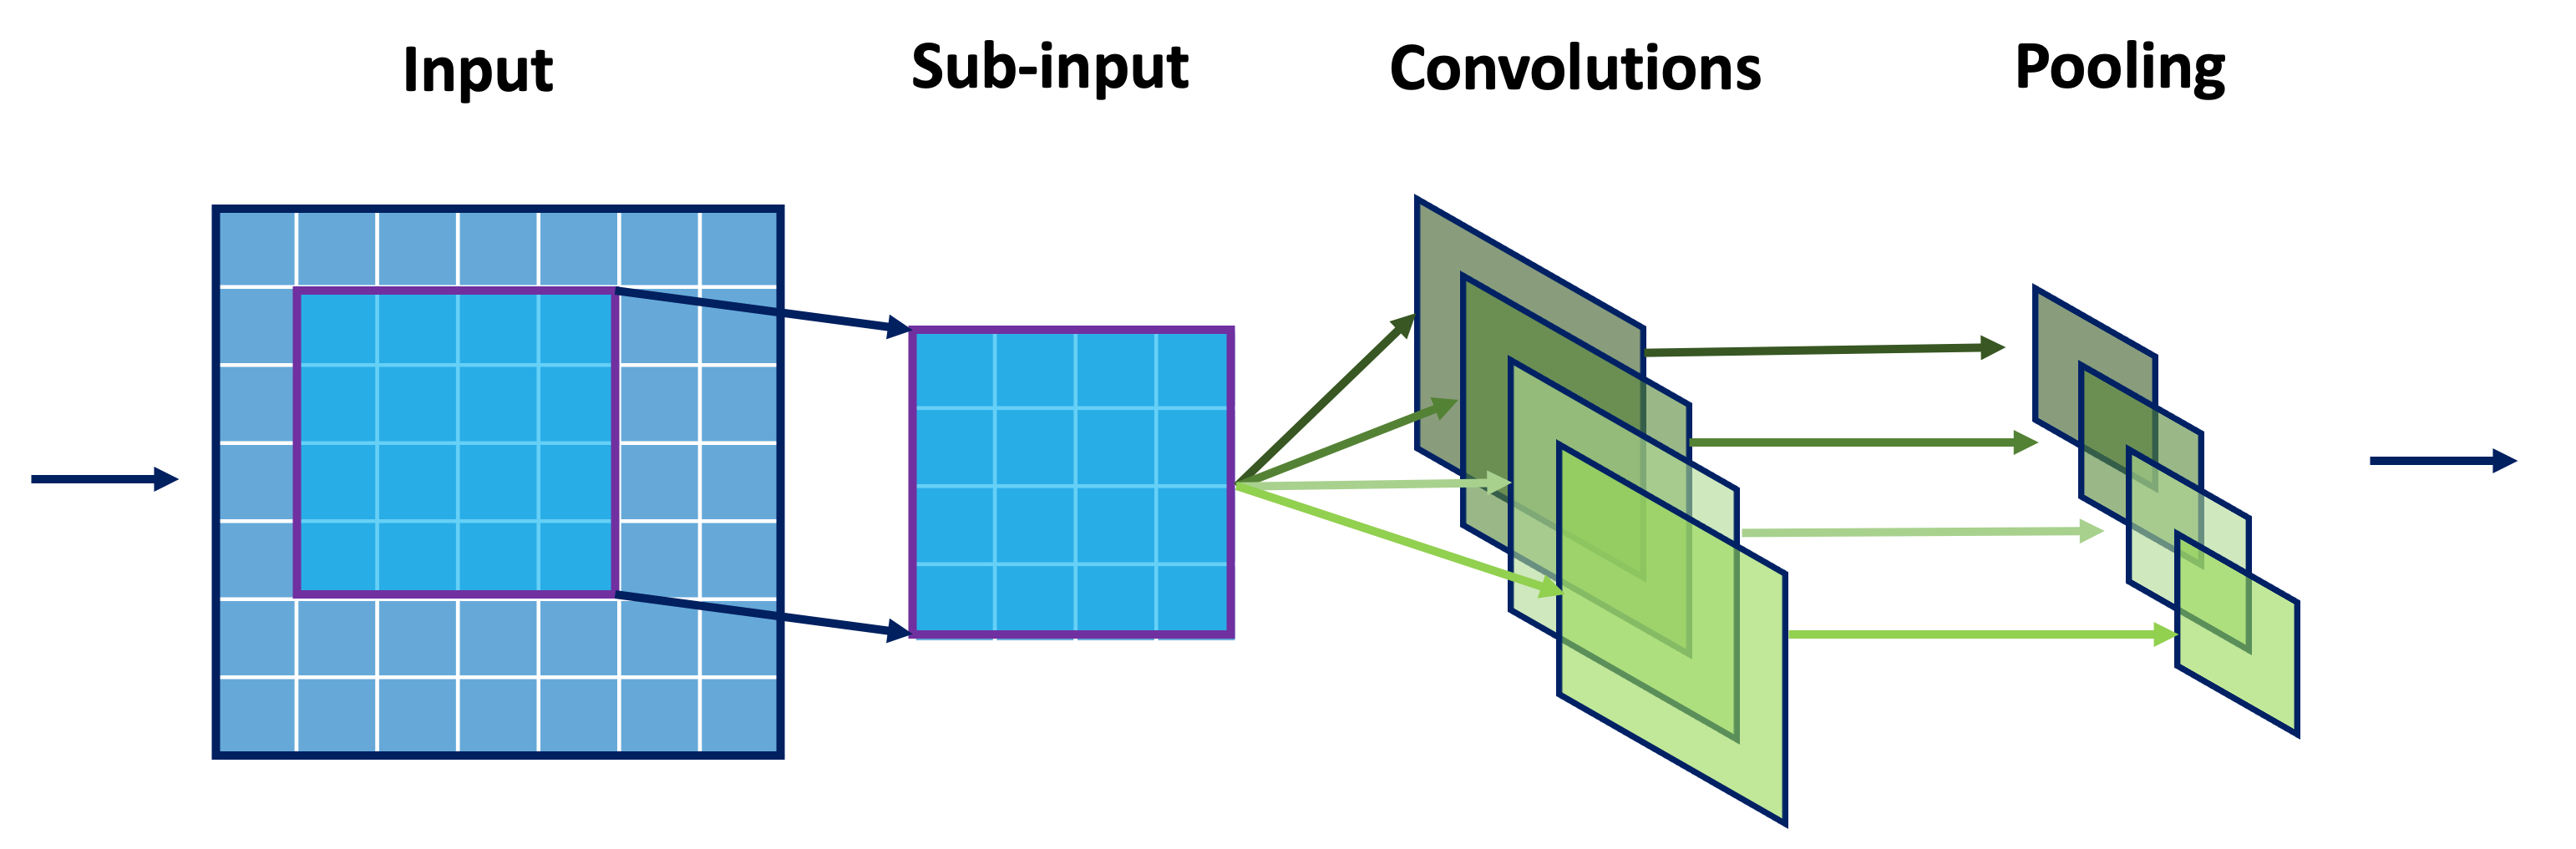
\includegraphics[scale=0.5]{Images/ML/cnn.png}
    \caption{A layer of a convolutional neural network, implementing a convolution with 4 kernels followed by a pooling operation. This design can be stacked to create deep architecture, and combined with a feed-forward neural network, after flattening the output as some depth, before reaching the final loss function layer.} 
    \label{fig:cnnDesign}
\end{figure}

The functioning of \gls{cnn} involves the use of convolutional layers to extract local patterns and features from input data. Convolutional operations are applied to the input data by multiplying a learnable \textit{kernel} or \textit{filter}, represented by a matrix of weights of smaller dimension than the total image, with an equally size subpart of the input and applying an activation function. Pooling layers are then used to reduce spatial dimensions and retain important features. Finally, fully connected layers combine the learned features to make predictions. Modern CNN architectures, such as AlexNet \cite{NIPS2012_c399862d}, and ResNet \cite{resNetPaper}, have demonstrated remarkable performance in various computer vision tasks.\\
A main advantage of the convolution operation on an image of size $x \times y$ is the reduction of the number of artificial neurons required to process the image, which helps to regularise the network.
\begin{itemize}
    \item A \gls{dnn} given the flatten image - the process of transformation the input image matrix $\mathbb{R}^{x} \times \mathbb{R}^{y}$ into a vector $\mathbb{R}^{x \times y}$- would requires $x \times y$ neurons. 
    \item A \gls{cnn} with kernel size $\alpha \times \beta$ would only require $\alpha \times \beta$ artificial neurons, that would be applied to different subpart of the image.
\end{itemize}
For example, for an image of size 100 $\times$ 100, a \gls{dnn} would require 10,000 weights while a \gls{cnn} could process the image with only 25 if a kernel of size 5 $\times$ 5 is used. Typical pooling functions are the \textit{maxPooling} or the \textit{sumPooling}, which, respectively, takes the largest element or the sum in the window of a size passed as A hyperparameter.\\
\textbf{Pros:}
\begin{itemize}
    \item \textit{Feature Learning:} CNNs automatically learn hierarchical representations of features, reducing the need for manual feature engineering.
    \item \textit{Spatial Hierarchies:} Convolutional and pooling layers enable the model to capture spatial hierarchies in the input data.
    \item \textit{State-of-the-Art Performance:} CNNs have achieved state-of-the-art performance in image classification, object detection, and segmentation tasks.
\end{itemize}

\textbf{Cons:}
\begin{itemize}
    \item \textit{Computational Complexity:} Training deep CNNs can be computationally intensive, requiring substantial resources.
    \item \textit{Large Datasets:} CNNs often require large labeled datasets for effective training, which may not be available for every application.
    \item \textit{Interpretability:} The internal workings of CNNs can be challenging to interpret, making them somewhat of a "black box."
\end{itemize}

\subsection{Graph Neural Networks}
Graph Neural Networks (\gls{gnn}) have gained significant attention for their ability to model and analyse complex relationships within graph-structured data \cite{graphNetRef}. Originally designed for tasks such as node classification and link prediction, \gls{gnn}s have found applications in diverse domains such as social networks, for recommendation systems, and physics, for modelling the dynamic of a $N$-body system, tracks reconstruction, and particle identification.\\
\gls{gnn}s operate on graph-structured data, where nodes or vertices represent entities, and edges represent relationships. The functioning of \gls{gnn}s involves iterative aggregation of information from neighbouring nodes, allowing them to capture local and global graph structures. This is achieved through the use of message-passing mechanisms. Furthermore, the information in a graph is not necessarily ordered as a sequence, thereby increasing the representation power of the model. Graphs are in fact able to to represent abritrary relational structures, as defined by the graph through its directional weighted edges \cite{graphInductiveBias}. A particular feature arising from this property is that graph are permutation equivariant: the order of nodes can be rearranged without impact. \\

\begin{figure}[h!]
    \center
    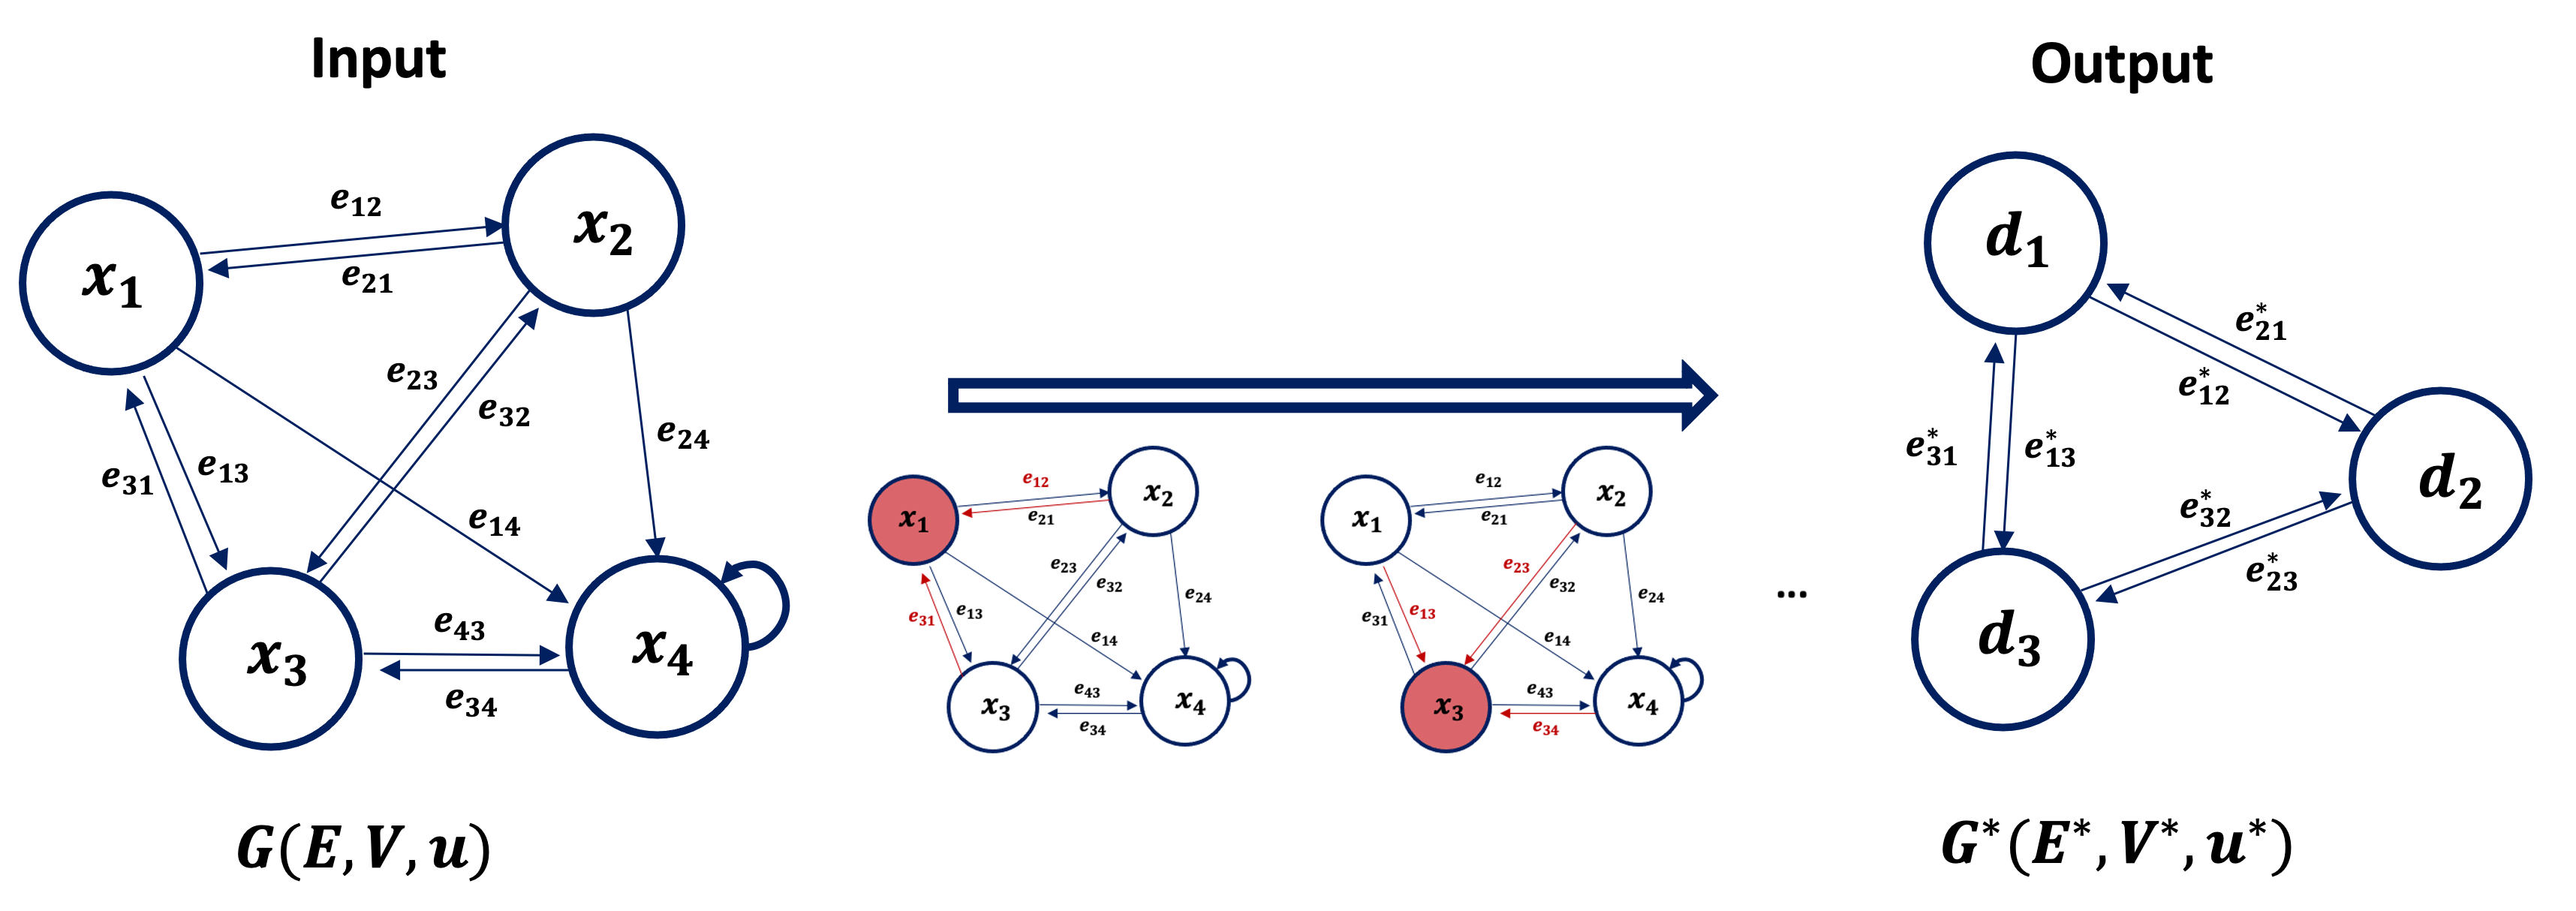
\includegraphics[scale=0.5]{Images/ML/gnn.png}
    \caption{A graph neural network on a directed graph $G(V, E, u)$ with a global representation $u$, four initial nodes $\in V$ and edges $e_{ij} \in E$ connecting nodes $i \rightarrow j$ (in the notation of the text, each node is given a different integer index $k$ and written $(e_k, r_k, s_k)$, with $r_k = j$ and $s_k = i$). By analysing the neighbours of each node, the graph is updated to a new graph $G^*(V^*, E^*, u^*)$.} 
    \label{fig:gnnScheme}
\end{figure}

Typically, a \gls{gnn} architecture consists of multiple layers of message passing operations. Each layer updates the node representations by aggregating information from neighbouring nodes, as schematised in Figure \ref{fig:gnnScheme}. Different architectures implement a different update process for the graph, with popular \gls{gnn} architectures being Graph Convolutional Networks (GCNs) \cite{gcnPaper} and Graph Attention Network \cite{velickovic2018graph}. In this thesis, the notation adopted is to represent a graph $G$ has a tuple of three entires:
\begin{enumerate}
    \item $E = \{(e_k, r_k, s_k)\}_{k=1:N^e}$ the set of edges, with each edge having a vector of features $e_k$ and storing the index of the receiver (sender) as $r_k$ ($s_k$).
    \item $V = \{v\}_{i=1:N^v}$ the set of nodes, each node having a vector of features $v_i$.
    \item $u$, a global attribute of the graph (also a vector of features). 
\end{enumerate}

\begin{algorithm}
    \caption{Steps of Computation in a Full Graph Network Block \cite{graphInductiveBias}}
    \label{algo:graph_network}

    \begin{algorithmic}[1]
    \Function{GraphNetwork}{$E, V, u$}
        \For{$k \in \{1 \ldots N^e\}$}
            \State $e^*_k \gets \phi^e(e_k, v_{r_k}, v_{s_k}, u)$
        \EndFor

        \For{$i \in \{1 \ldots N^n\}$}
            \State Let $E_i^* = \{(e^*_k, r_k, s_k)\}$ for $k = 1 : N^e$ where $r_k = i$
            \State $\overline{e^*_i} \gets \rho^{e \to v}(E^*_i)$
            \State $v^*_i \gets \phi^v(\overline{e^*_i}, v_i, u)$
        \EndFor

        \State Let $V^* = \{v^*\}_{i=1}^{N^v}$
        \State Let $E^* = \{(e^*_k, r_k, s_k)\}_{k=1}^{N^e}$
        \State $\overline{e^*} \gets \rho_{e \to u}(E^*)$
        \State $\overline{v^*} \gets \rho_{v \to u}(V^*)$
        \State $u^* \gets \phi_u(\overline{e^*}, \overline{v^*}, u)$

        \State \Return $(E^*, V^*, u^*)$
    \EndFunction
    \end{algorithmic}
\end{algorithm}

The most general graph update algorithm to describe a step fo computation of a full \gls{gnn} block is described in Algorithm \ref{algo:graph_network}. Essentially, at a given time step a graph $G$ is updated into a new graph $G^*$ by first updating the edges $e$ and then modifying the nodes $v$ and the global features. The update rule leverages different neural network $\phi$ and aggregation function $\rho$ - accepting variable number of input with permutation invariance to output a single element per group, typically sum or max pooling - to update the graph: 
\begin{itemize}
    \item The edges with a \gls{dnn} $\phi^e$, mapping each of the input edge, the couple of receiver and sender nodes and the global state $u$ to output a new edge feature vector $e^*_k$: $e^*_k = \phi^e(e_k, v_{r_k}, v_{s_k}, u)$
    \item To update vertex $i$ represented by $v_i$, the edges connecting to $i$ ($i == r_k$) are pooled locally over the node as $\overline{e^*_i} = \rho^{e \rightarrow v}$
    \item The vertex is then updated with a \gls{dnn} $\phi^v$, mapping the pooled representation of the edge $\overline{e^*_i}$, the input vertex feature $v_i$ and the global representation $u$: $v^*_i = \phi^v(\overline{e^*_i}, v_i, u)$
    \item The set of edges is updated by a global pooling $E^* = \rho^{e \rightarrow u}$
    \item The set of vertices is updated by a global pooling $V^* = \rho^{v \rightarrow u}$
    \item The global representation is updated by \gls{dnn} $\phi^u$ mapping $u^* = \phi_u(\overline{e^*}, \overline{v^*}, u)$ using the updated edges and vertices. 
\end{itemize} 
This formulation of a graph as a message-passing with edges update device is the most complete architecture. The design is however flexible: for example, \gls{rnn}s or \gls{cnn}s can be used instead of \gls{dnn}. Furthemore, many specialisations of the structures exist to reduce the degree of complexity of the model and avoid overfitting or converge issues, as listed in Figure \ref{fig:diverseGNN}. A notable example for this thesis is the Deep Set architecture \cite{NIPS2017f22e4747}, designed to runs on set. It essentially simplifies the graph network by dropping altogether the edges and considering instead a fully connected graph with static edges, with an update of the global representation only based on pooled node information: 
\[v^*_i = \phi^v(\overline{e^*_i}, v_i, u) = \phi^v(v_i, u)  \] 
\[\overline{V^*} = \rho^{v \rightarrow u} = \sum_i v^*_i\] 
\[u^* = \phi_u(\overline{e^*}, \overline{v^*}, u) = \phi_u( \overline{v^*}, u), \] PointNet, a \gls{gnn} designed for set of 3D points analyses, deploys a similar strategy with max-aggreagtion instead of sum pooling after updating the nodes in two steps \cite{pointNet}.  

\begin{figure}[h!]
    \centering
    \begin{subfigure}[b]{0.49\textwidth}
        \centering
        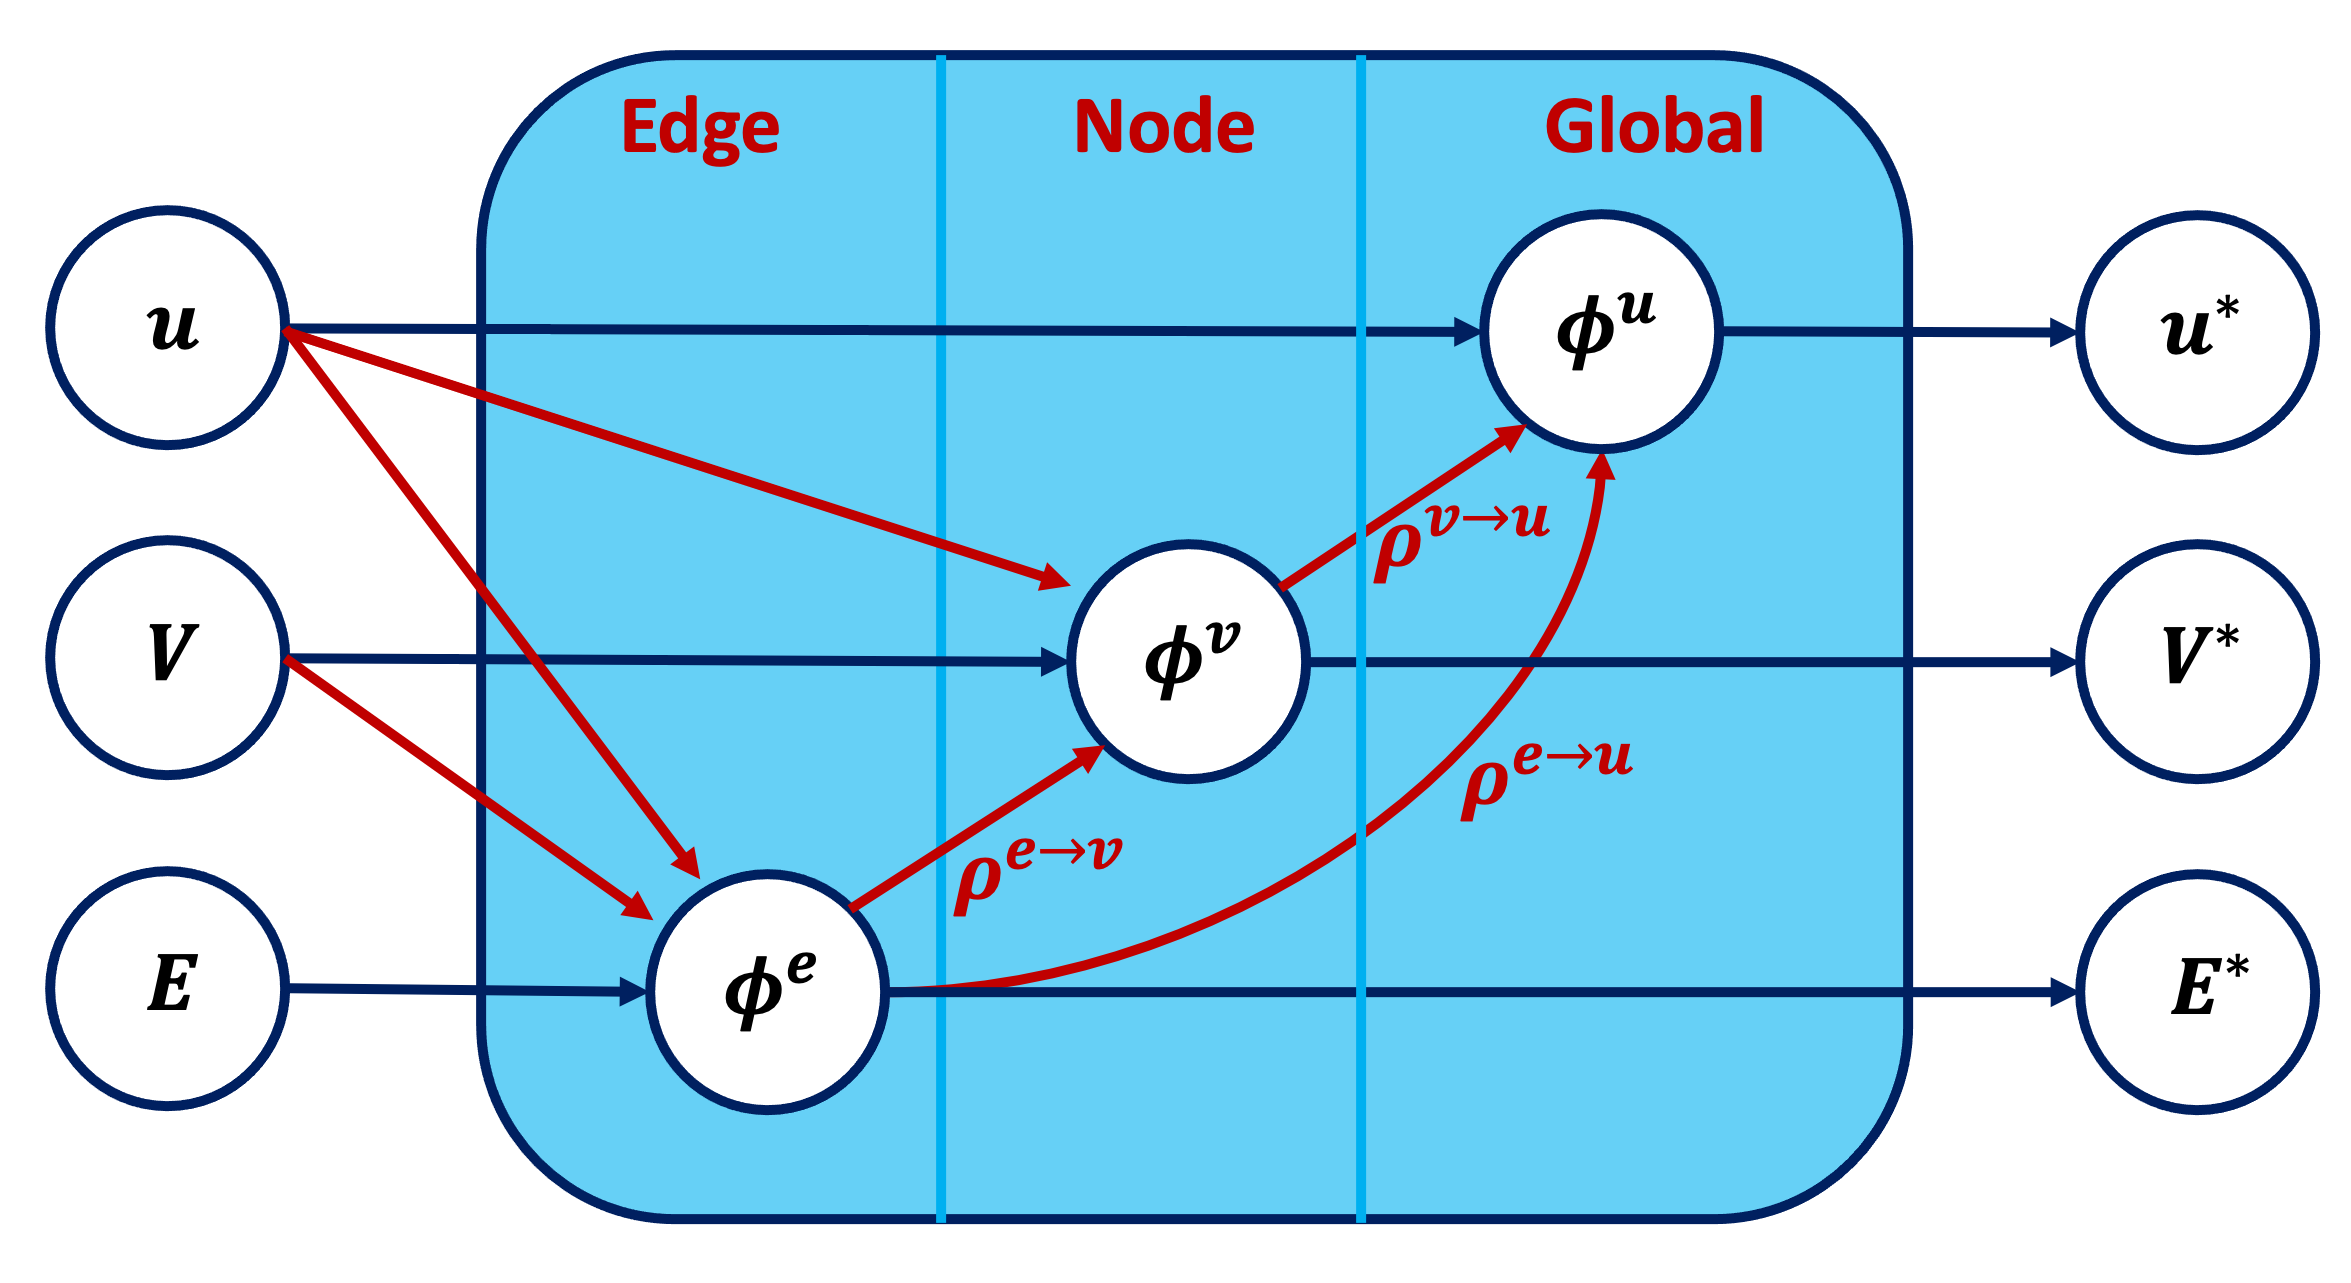
\includegraphics[scale=0.43]{Images/ML/fullGNN.png}
        \caption{Full \gls{gnn}.} 
        \label{fig:diverseGNNfull}
    \end{subfigure}
    \hfill
    \begin{subfigure}[b]{0.49\textwidth}
        \centering
        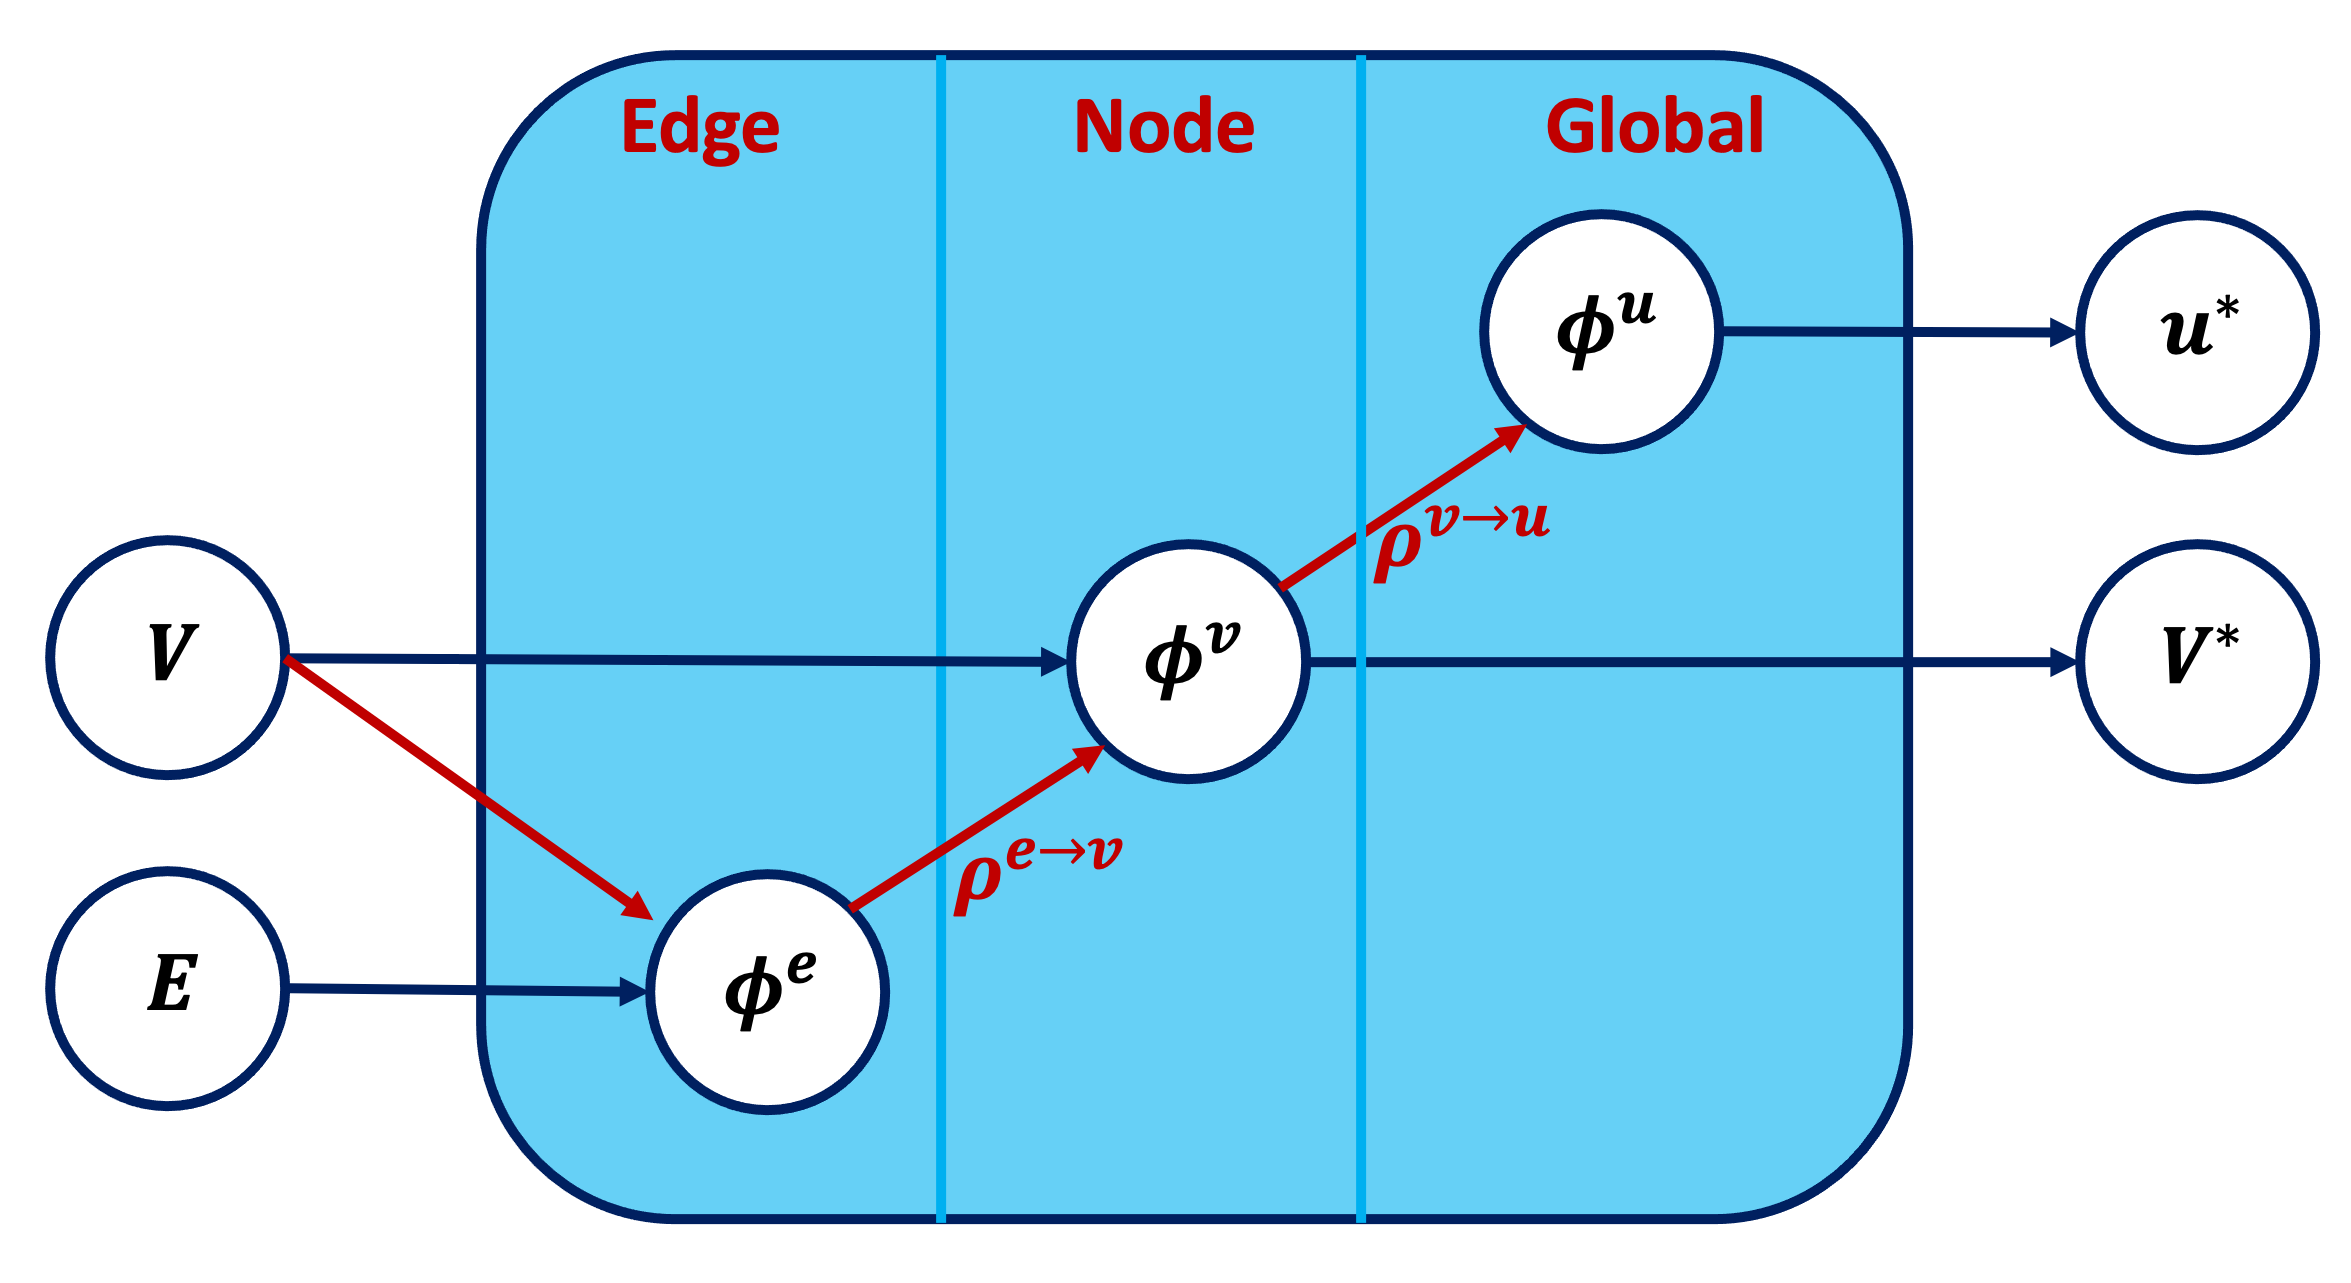
\includegraphics[scale=0.43]{Images/ML/messagepassingNN.png}
        \caption{Message-passing \gls{gnn}.} 
        \label{fig:pullsFTAGmp}
    \end{subfigure}
    \\  % newline
    \begin{subfigure}[b]{0.49\textwidth}
        \centering
        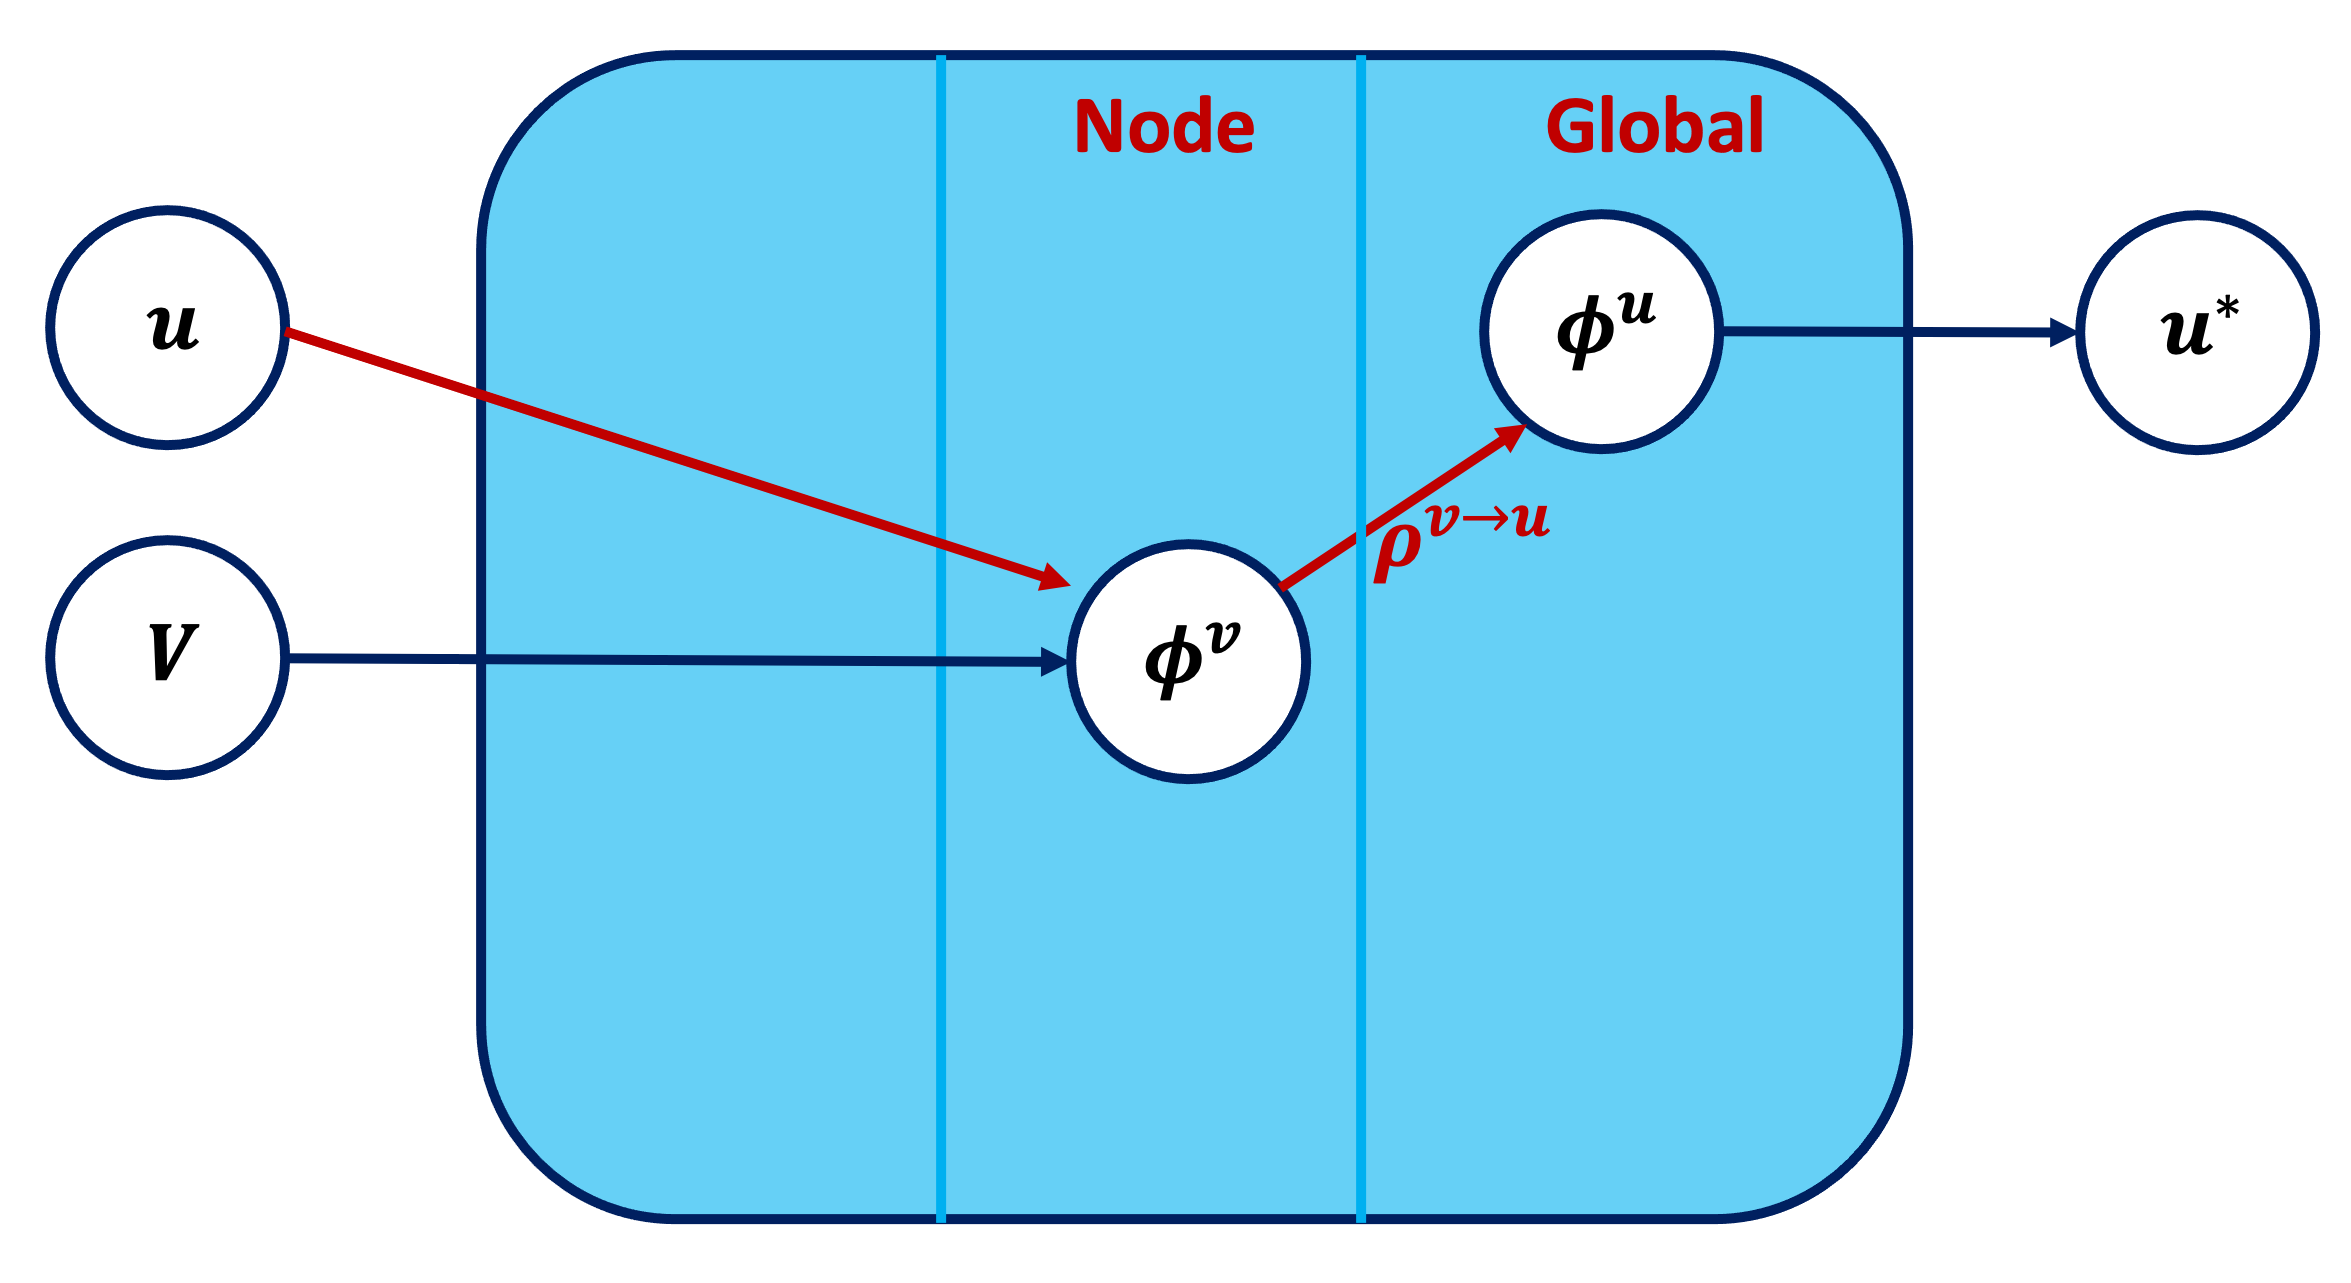
\includegraphics[scale=0.43]{Images/ML/deepSet.png}
        \caption{Deep Set.} 
        \label{fig:deepSetFig}
    \end{subfigure}
    \hfill
    \begin{subfigure}[b]{0.49\textwidth}
        \centering
        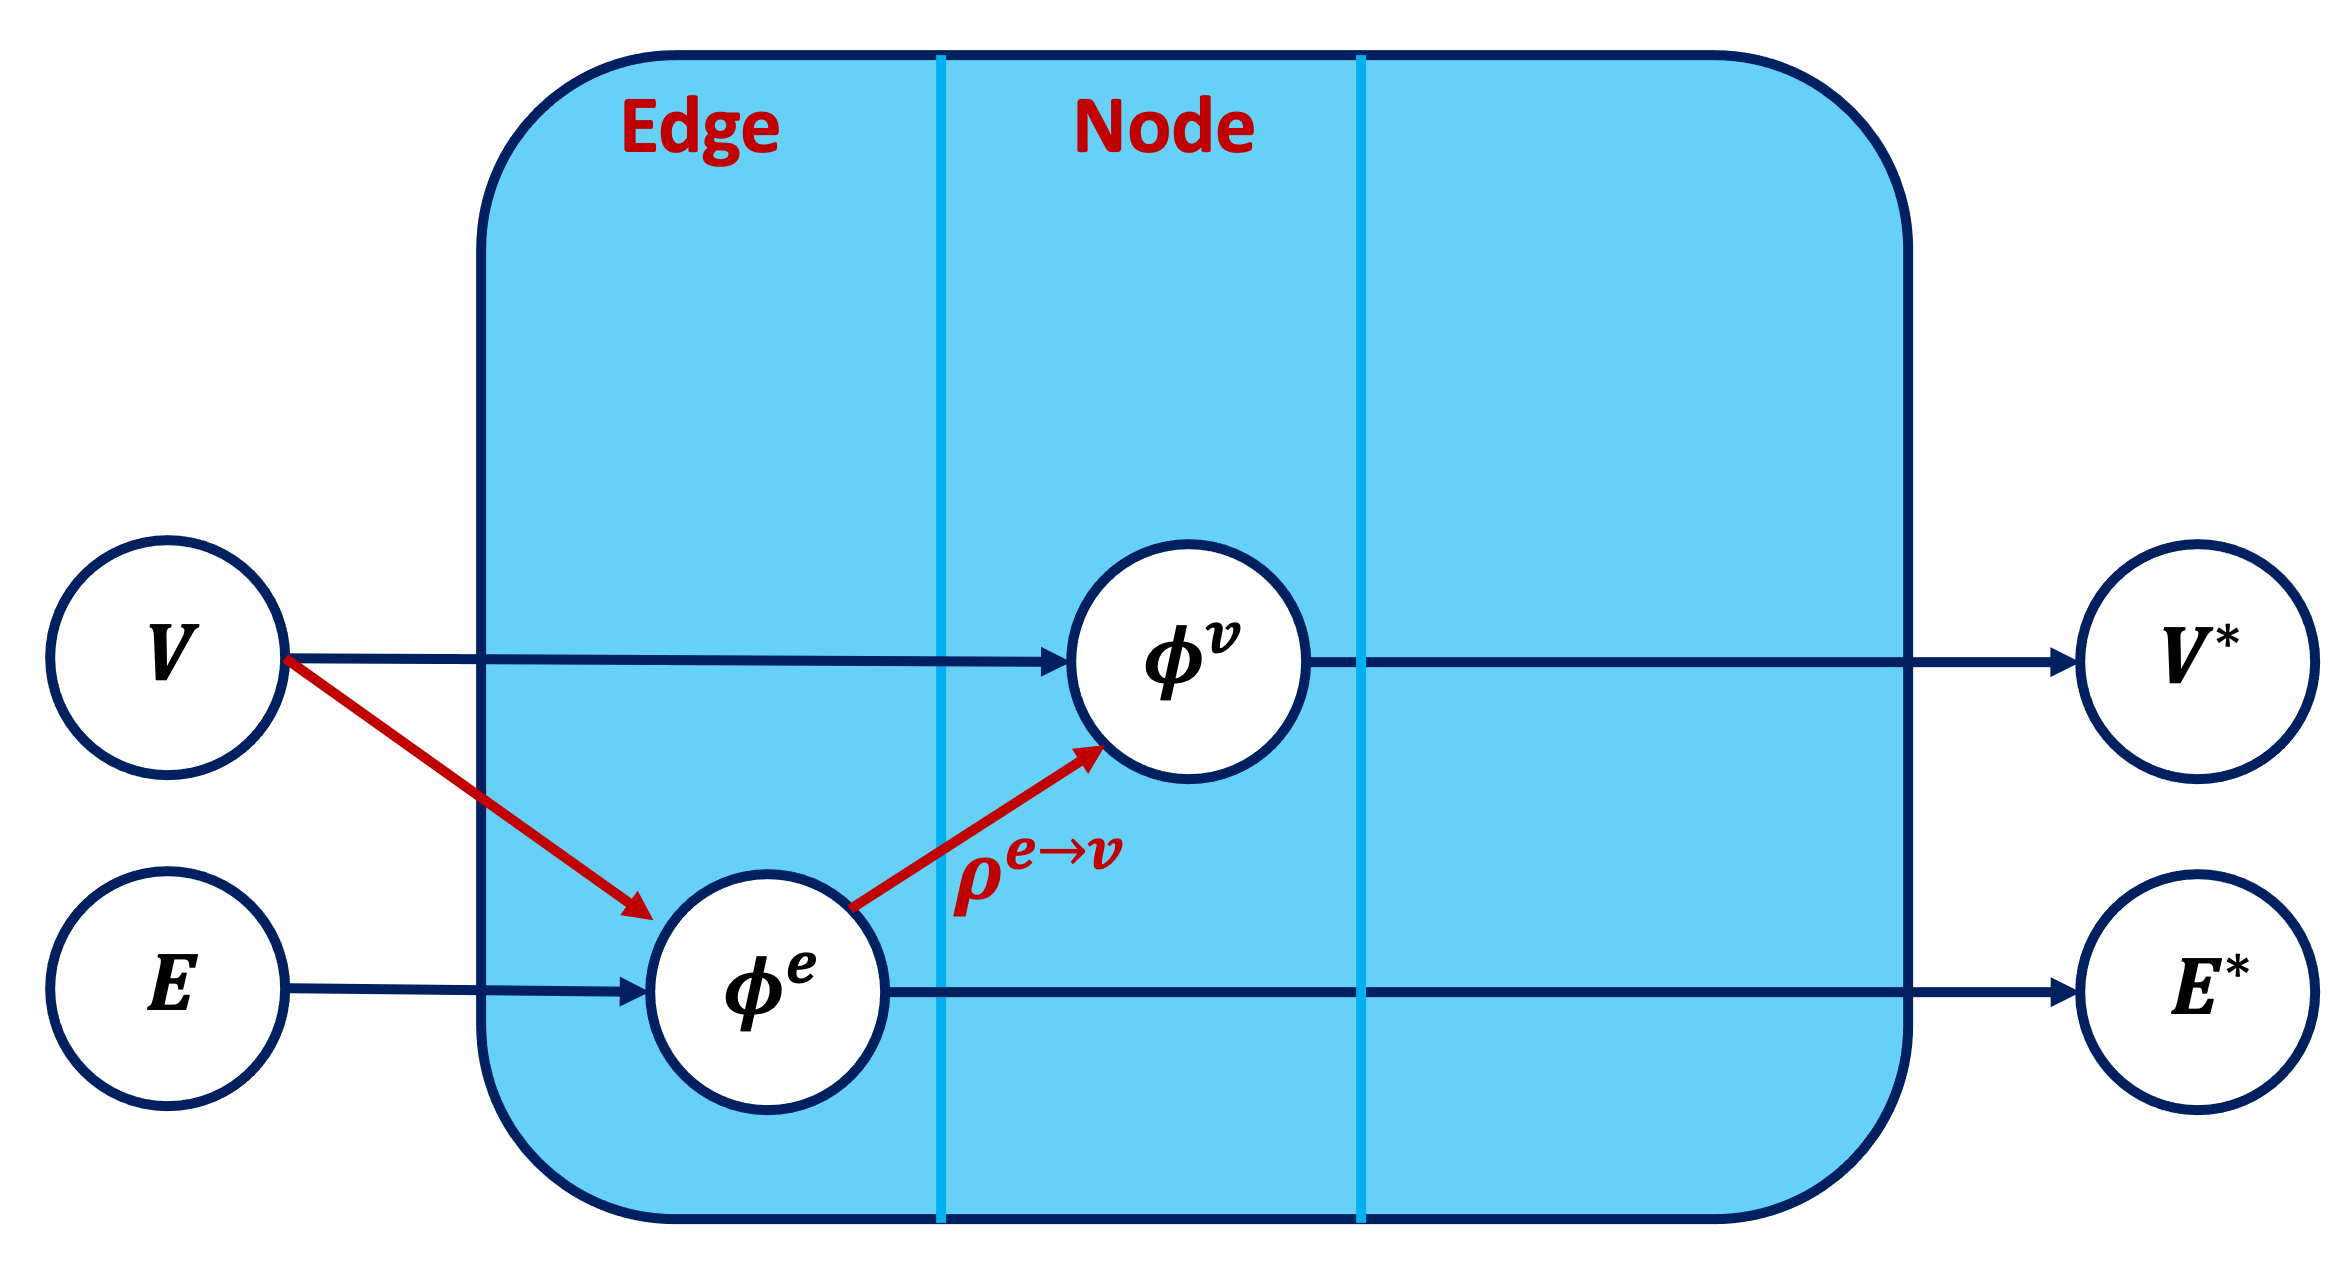
\includegraphics[scale=0.43]{Images/ML/nlnn.png}
        \caption{Non-local \gls{nn}.} 
        \label{fig:pullsFTAGmp}
    \end{subfigure}\\
    \caption{Some of the different types of \gls{gnn} update rules, defining different \gls{gnn} architecture \cite{graphInductiveBias}.}
    \label{fig:diverseGNN}
\end{figure} 

A different approach is that presented in \cite{nlnnPaper} introducing non-local neural network to unify different types of \textit{attention}-based architecture. Attention is an essential feature of modern deep learning architecture: it refers to how an element is given a weighted version of the inputs, with weights standing for the degree of attention to be given to each different part of the input. This concept is not restricted to \gls{gnn} but is easily encapsulated in this formalism. As will be shown in the next section, the transformer is a special case of this non-local \gls{nn} family. Here, for the sake of concisness, only the \gls{gat} will be introduced \cite{velickovic2018graph}. \gls{gat} introduce the attention mechanism by having a learnable weighting of the neighbour of the node being updated. When updating node $v_i$, a score is derived computed for each of the connected neigbour of $v_i$ by a \gls{nn} mapping: \[e(v_i, v_j) = \phi(v_i, v_j) = a^T \text{ leakyReLu}([W v_i, Wv_j]),\] where leakyReLu is a modification of the \gls{relu} with negative leakage (leakyReLu = $max(\alpha x, x)$, with $0 \leq \alpha < 1$), the nodes $v \in \mathbb{R}^d$, the embedding of the graph mapping the node to $d'$ with  $a \in \mathbb{R}^{2d'}$ and $W \in \mathbb{R}^{d' \times d}$ being the learnable parameters ($[,]$ is concatenation of the elements). These scores are then combined for each node $i$ over its neighbours $\{j\}$ to give attention scores $\alpha_{ij}$: \[ \alpha_{ij} = \text{softmax}_j (e(v_i, v_j)) = \frac{\exp(e(v_i, v_j))}{\sum_{j' \in \text{neighours of i}}e(v_i, v_{j'})}.\] The final step is to leverage these attention weights when updating each node $v_i$: \[v^*_i = \sigma\left(\sum_{j} \alpha_{ij} . W v_j \right),\] where the sum over $j$ is taken over neighbouring nodes of $i$ and $\sigma$ is any activation function.\\
Some pros and cons of \gls{gnn}s are:

\textbf{Pros:}
\begin{itemize}
    \item \textit{Modeling Graph Structure:} \gls{gnn}s naturally handle graph-structured data, making them well-suited for tasks involving relationships between entities.
    \item \textit{Transferability:} Pre-trained \gls{gnn} models on one graph can be fine-tuned for related tasks on another graph.
    \item \textit{State-of-the-Art Performance:} \gls{gnn}s have achieved state-of-the-art results in various graph-related tasks, including node classification and link prediction.
\end{itemize}

\textbf{Cons:}
\begin{itemize}
    \item \textit{Computational Complexity:} Training \gls{gnn}s can be computationally expensive, particularly for large graphs.
    \item \textit{Limited Global Context:} Some \gls{gnn}s architectures may struggle to capture long-range dependencies in graphs, limiting their ability to consider global context.
    \item \textit{Interpretability:} Similar to other deep learning models, GNNs may lack interpretability, making it challenging to understand the learned representations.
\end{itemize}

\subsection{The rise of the Transformers}\label{sec:transformer}

The Transformer architecture, introduced in 2017 \cite{NIPS_transformerPaper}, has become a foundational model for \gls{nlp} tasks. It has significantly impacted the field, enabling the development of state-of-the-art models such as BERT \cite{devlin-etal-2019-bert} and GPT \cite{radford2018improving}. Note that the transformer is also spearheading a revolution in computer vision tasks thanks to the generalisation of the architecture into the Vision Transformer (ViT) \cite{vitPaper}.

The Transformer architecture is based on the mechanism of self-attention introduced in the last section. As mentionned in section \ref{sec:RNN} on \gls{rnn}, it abandons sequential processing and adopts a parallelised approach, allowing for efficient computation on parallelisable hardware. The key components of the Transformer are the self-attention mechanism and position-wise feedforward networks. The self-attention mechanism allows the model to weigh the importance of different words or tokens in a sequence when making predictions for a specific token. This mechanism enables the model to capture long-range dependencies in the input data without the added complexity of \gls{lstm} or \gls{gru}. Strictly speaking, the input of a transformer is a sequence that is not ordered. In \gls{nlp}, the importance of ordering is built-in using position-wise embedding to let the network decypher the index of the token in the input sequence. For the computer vision case, the Vision Transformer splits an input image $x$ into patches of fixed size, that are flattened into a vector and mapped with a learnable positional embedding.

\begin{figure}[h!]
    \center
    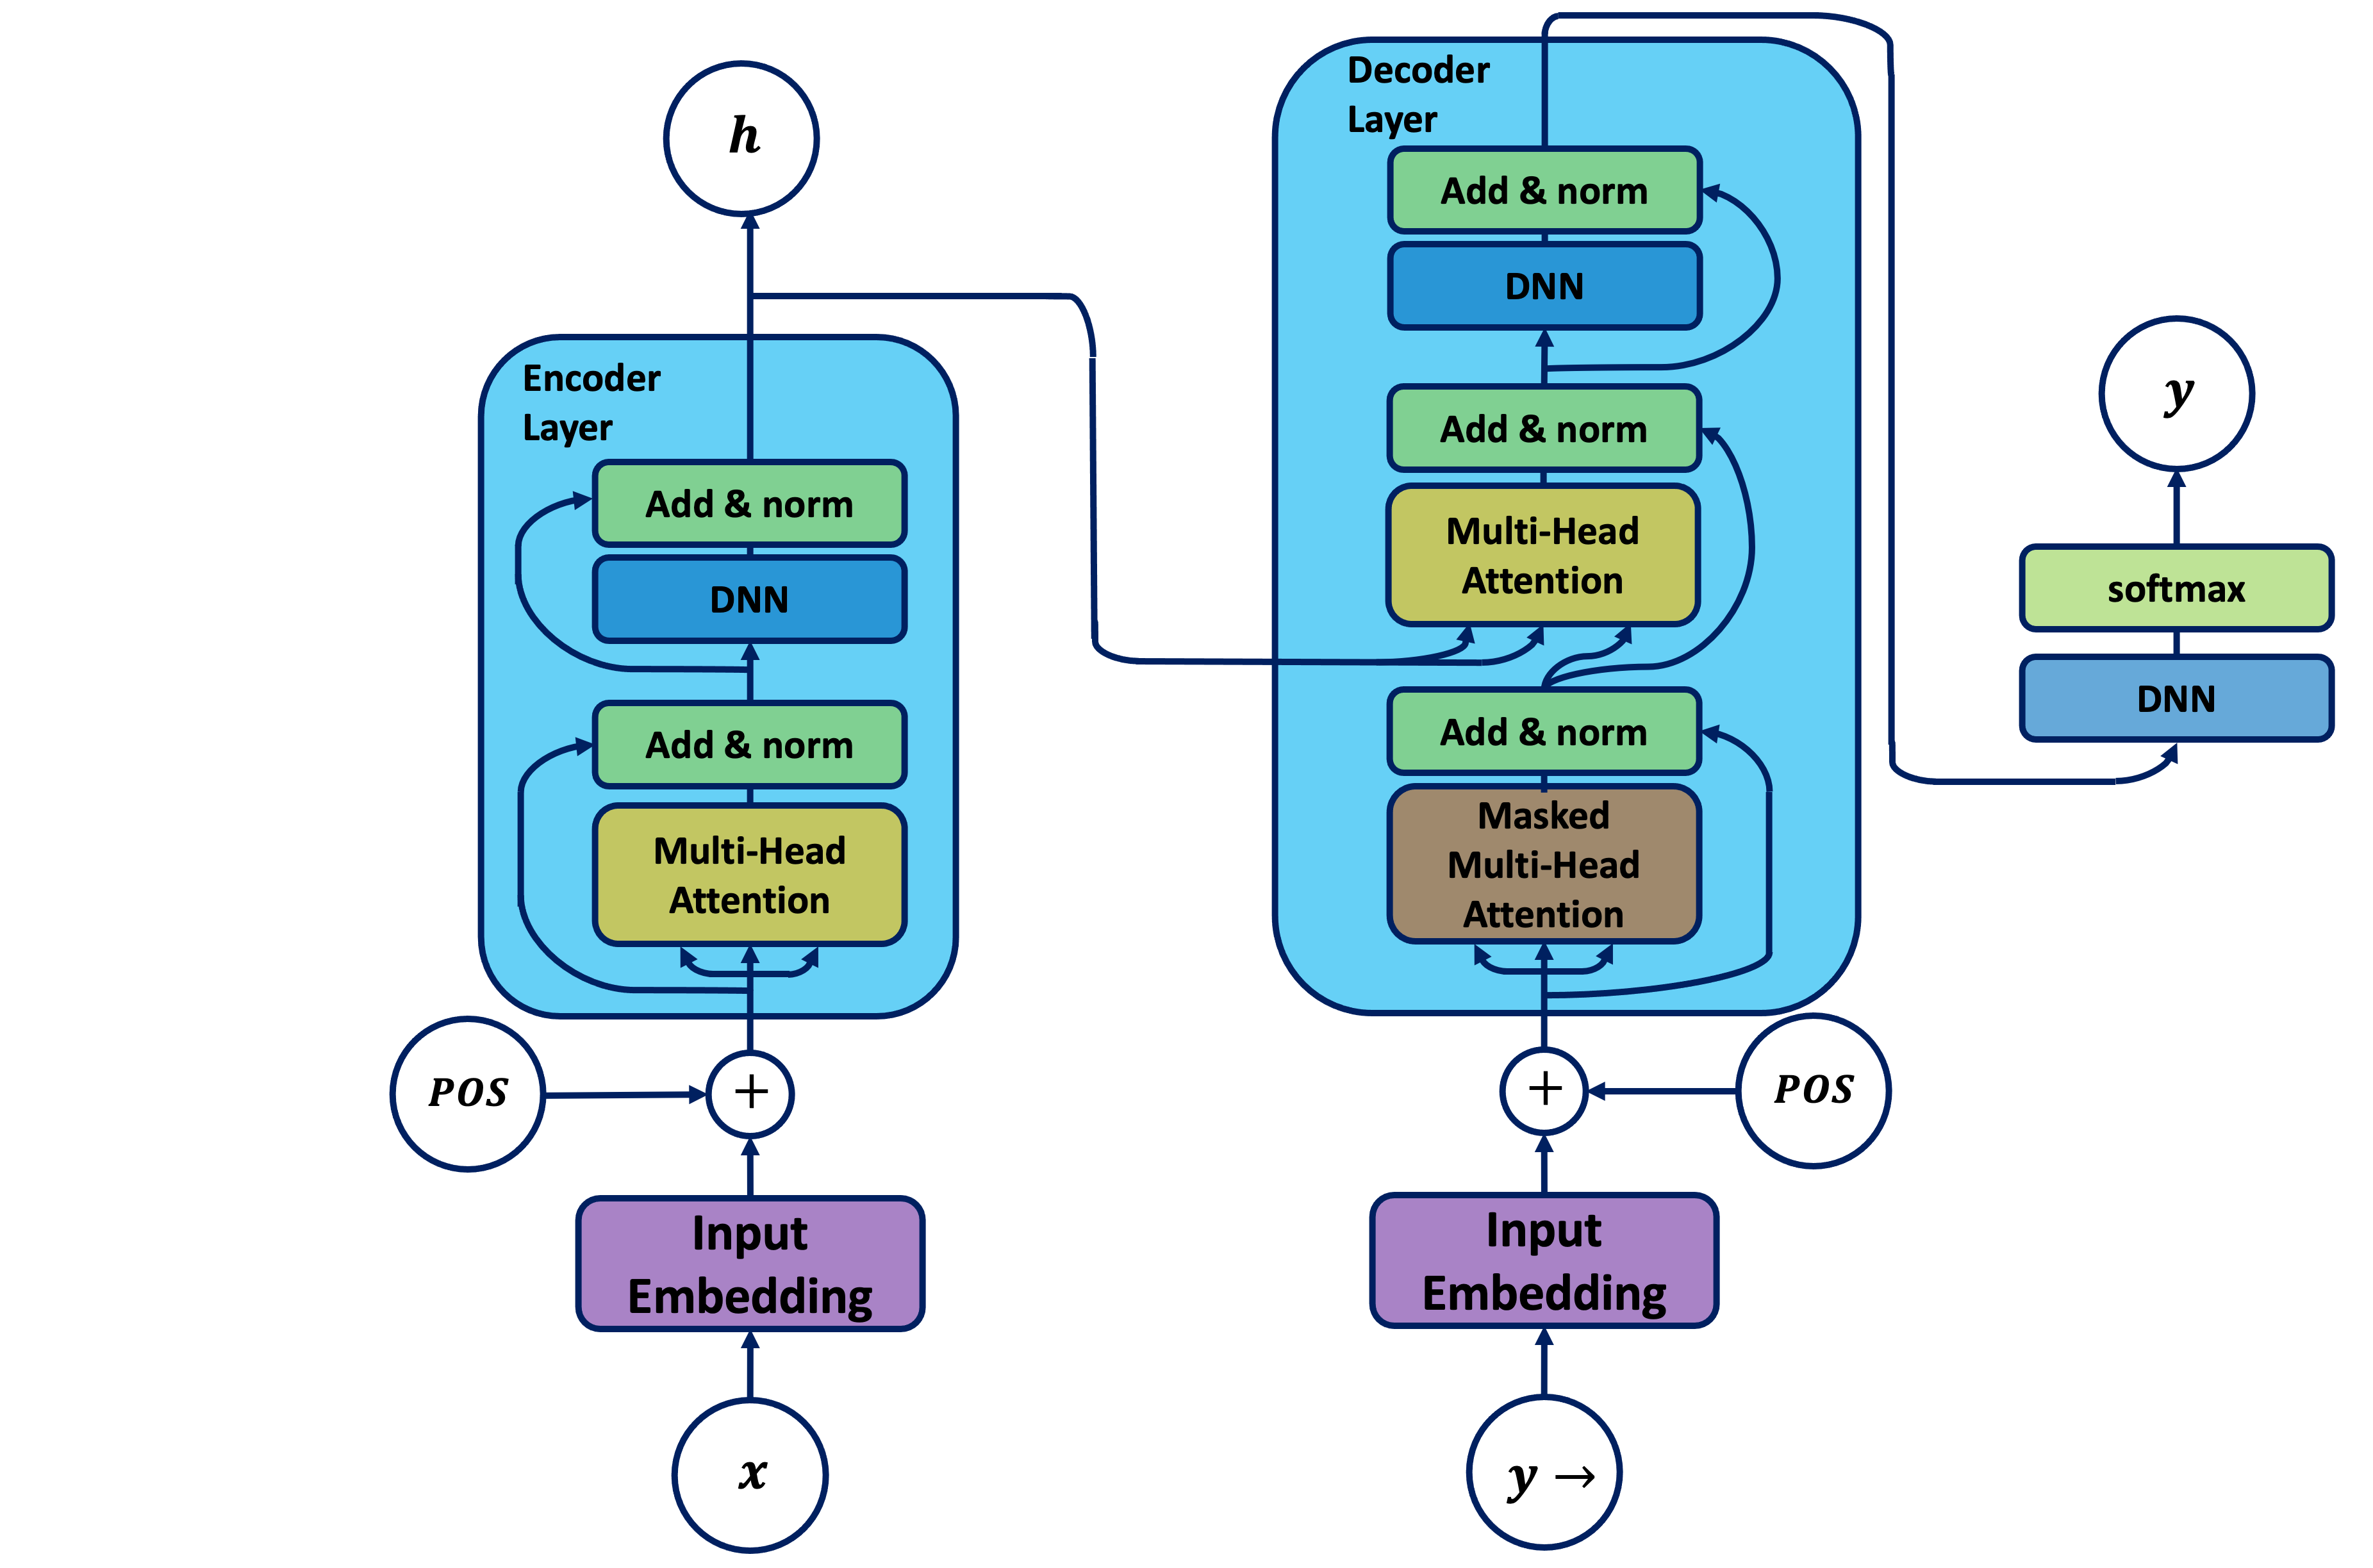
\includegraphics[scale=0.5]{Images/ML/transformer.png}
    \caption{The full transformer architecture, combining an encoder and a decoder each made of an arbitrary number of layers. The input $x$ is first embedded with a dedicated mapping which can, when order matters, be supplemented with positional embedding. The encoder generates an internal representation $h$ that is passed to the decoder. This last component produces the next output using the internal representation $y$ and the output shifted to the right - to force output token to only access prior information. } 
    \label{fig:tranfoArchi}
\end{figure}

As presented in Figure \ref{fig:tranfoArchi}, the general Transformer architecture consists of an encoder and a decoder, the main feature of auto-encoders model. The decoder works in an autoregressive way, combining the current output with an internal representation $h$ built by the encoder to generate new output tokens $y$. Both the encoder and decoder are composed of multiple layers, each containing a multi-head self-attention mechanism and position-wise feedforward networks (\gls{dnn}). The decoder is further endowed with a masked attention layer, for the output to compute self-attention with information accessible prior to the token's position. The attention mechanism allows the model to focus on different parts of the input sequence, while the feedforward networks provide additional non-linear transformations. Residual connexions are added to let the gradients propagate efficiently in depth and layer normalisation is used after each block to avoid vanishing or exploding gradients and improve training speed \cite{ba2016layer}. This type of normalisation scales each activation (each neuron) by substracting the empirical mean and dividing by the standard deviation per datapoint. \\
The attention mechanism maps the queries and a set of key-value pairs to an output as defined in Equation \ref{eq:scdotatt} and schematised in Figure \ref{fig:scaledDotAtt}, with query $Q \in \mathbb{R}^{d_q \times d_k}$, key $K \in \mathbb{R}^{d_k \times d_v}$, and value $V \in \mathbb{R}^{d_v}$ and the output is a vector $\mathbb{R}^{d_q \times d_v}$. This combines $d_q$ different queries of the $d_k$ keys mapping to $d_v$ values. Equation \ref{eq:scdotatt} is weighted sum of the values, based on a compatibilty function established by comparing the queries and keys:
\begin{equation}\label{eq:scdotatt}
    \text{Attention}(Q, K, V) = \text{softmax}\left( \frac{Q^T . K}{\sqrt{d_k}}\right) V,
\end{equation} 
where the scaling by $\sqrt{d_k}$ is implemented to reduce the magnitude of the dot product $Q^T K$ and avoid landing in regions of saturation of the following softmax. This scaled dot-product attentino mechanism leverages the extensive optimisation of the associated matrix multiplication, making this operation less time and memory demanding than using a \gls{dnn} mapping to compute the attention - a technique referred to as \textit{additive attention} \cite{Bahdanau2014NeuralMT}. As shown in Figure \ref{fig:mulitheadAtt}, multi-head attention runs the dot-product self-attention in parallel for $h$ different heads, each head $h_i$ implementing a separate projection from the input $x \in \mathbb{R}^{N \times d}$ to $Q, K, V$ with linear transformation of respective weights $W_i^Q \in \mathbb{R}^{d \times d_k}$, $W_i^K \in \mathbb{R}^{d \times d_k}$, and $W_i^Q \in \mathbb{R}^{d \times d_v}$, where $N$ is the length of the sequence, $d$ is the model dimension and $h$ the number of heads: \[Q = xW_i^Q,\] \[K = xW_i^K,\] \[V = xW_i^V,\] \[h_i = \text{Attention}(QW_i^Q, KW_i^K, VW_i^V).\] The multi-head module then concatenates the $h$ different heads outputs and applies another linear tranformation of parameters $W^O \in \mathbb{R}^{hd_v \times d}$: \[\text{Multi-Head Attention}(Q, K, V) = \text{Concatenate}(h_1, ...h_h)W^o .\] Self-attention is a special case in which the multi-head does not receive a tuple $(Q, K, V)$ but a single input $x \in \mathbb{R}^{N \times d_v}$ that is mapped out to the tuple. 

\begin{figure}[h!]
    \centering
    \begin{subfigure}[b]{0.49\textwidth}
        \centering
        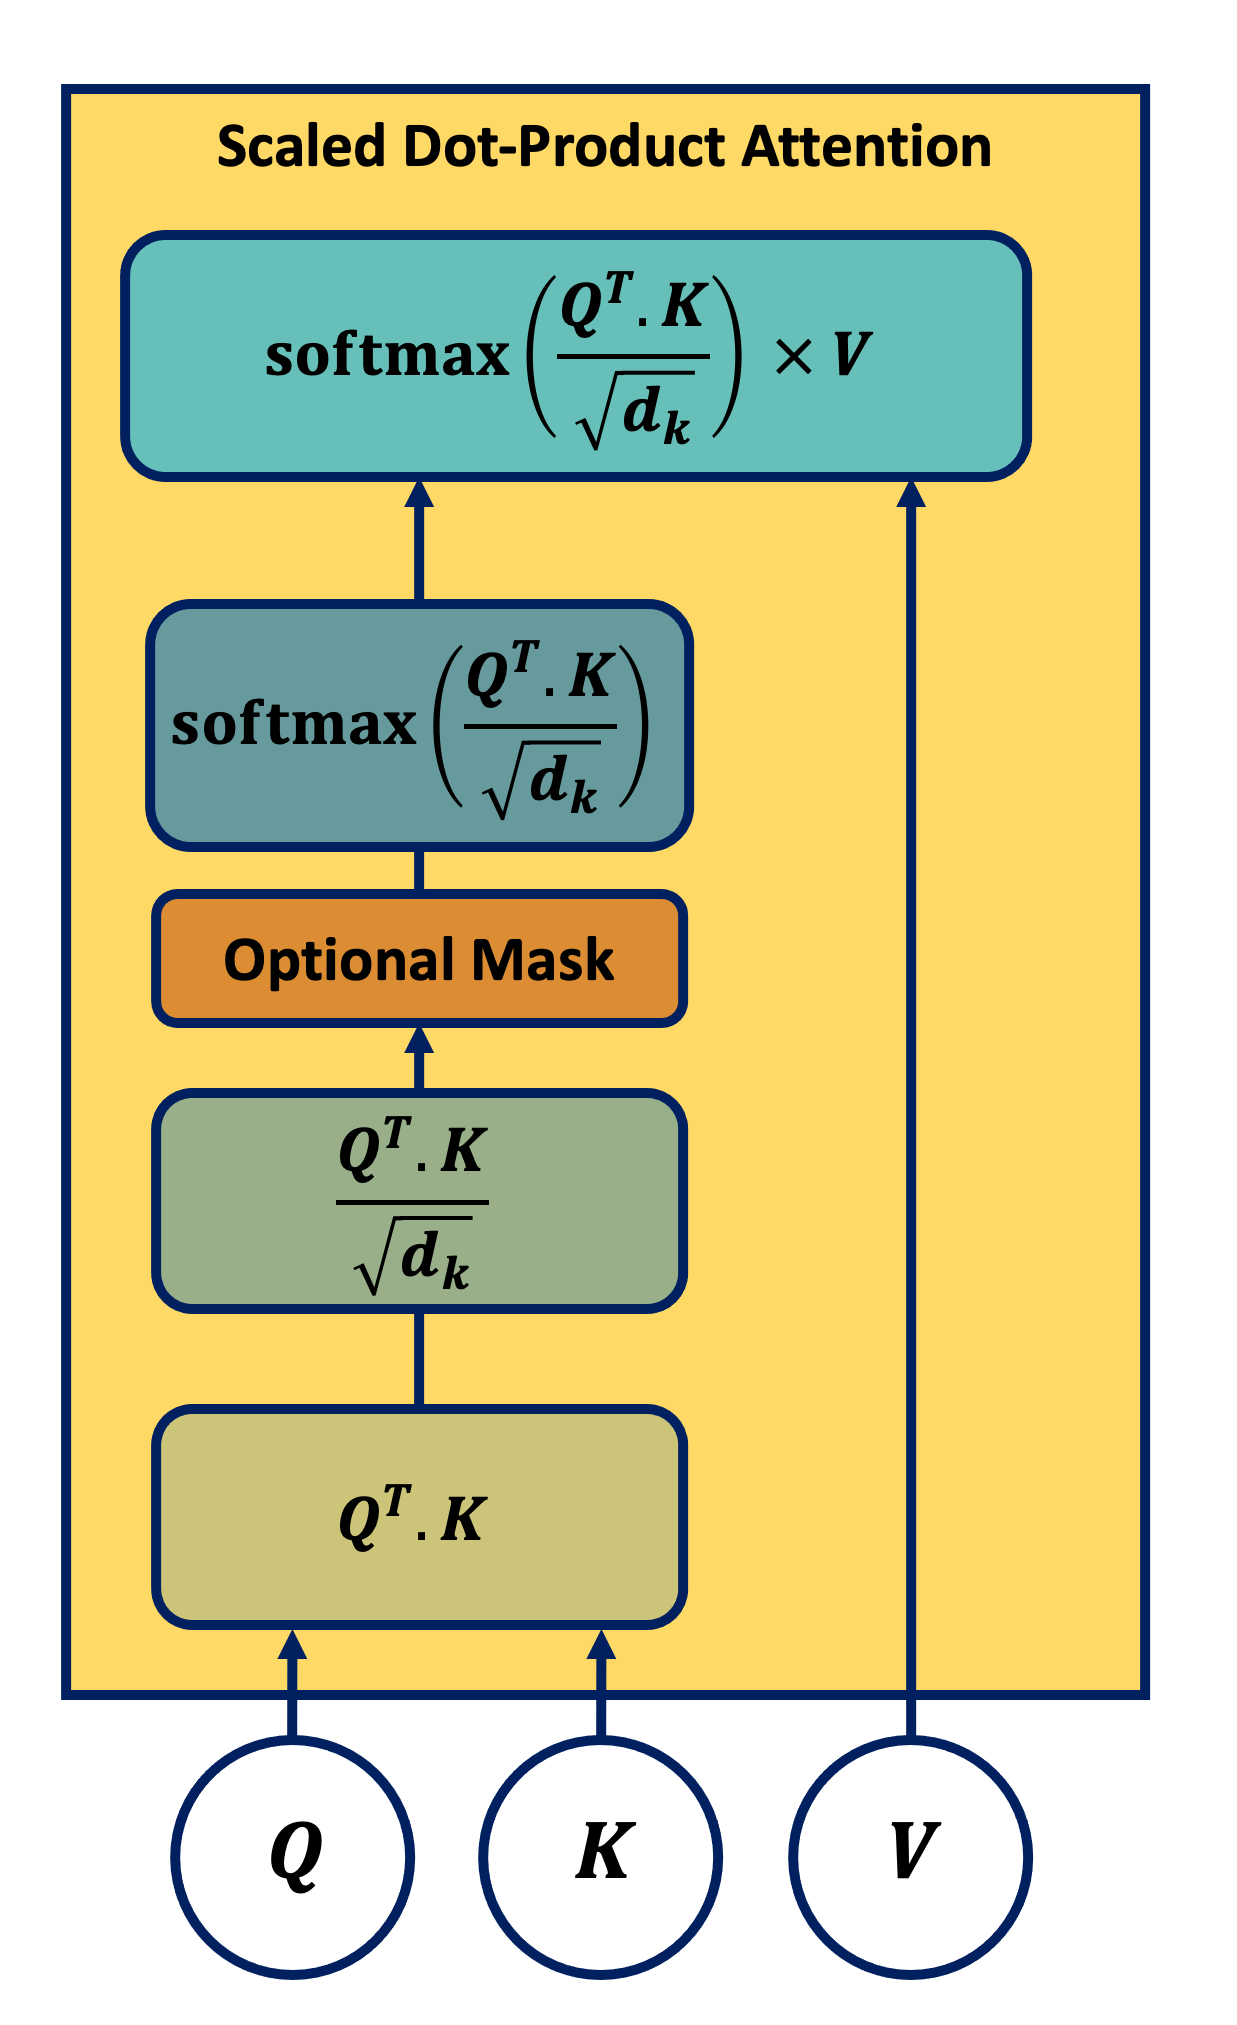
\includegraphics[scale=0.65]{Images/ML/scaledDotAtt.png}
        \caption{Scaled dot-product attention with optional masking.} 
        \label{fig:scaledDotAtt}
    \end{subfigure}
    \hfill
    \begin{subfigure}[b]{0.5\textwidth}
        \centering
        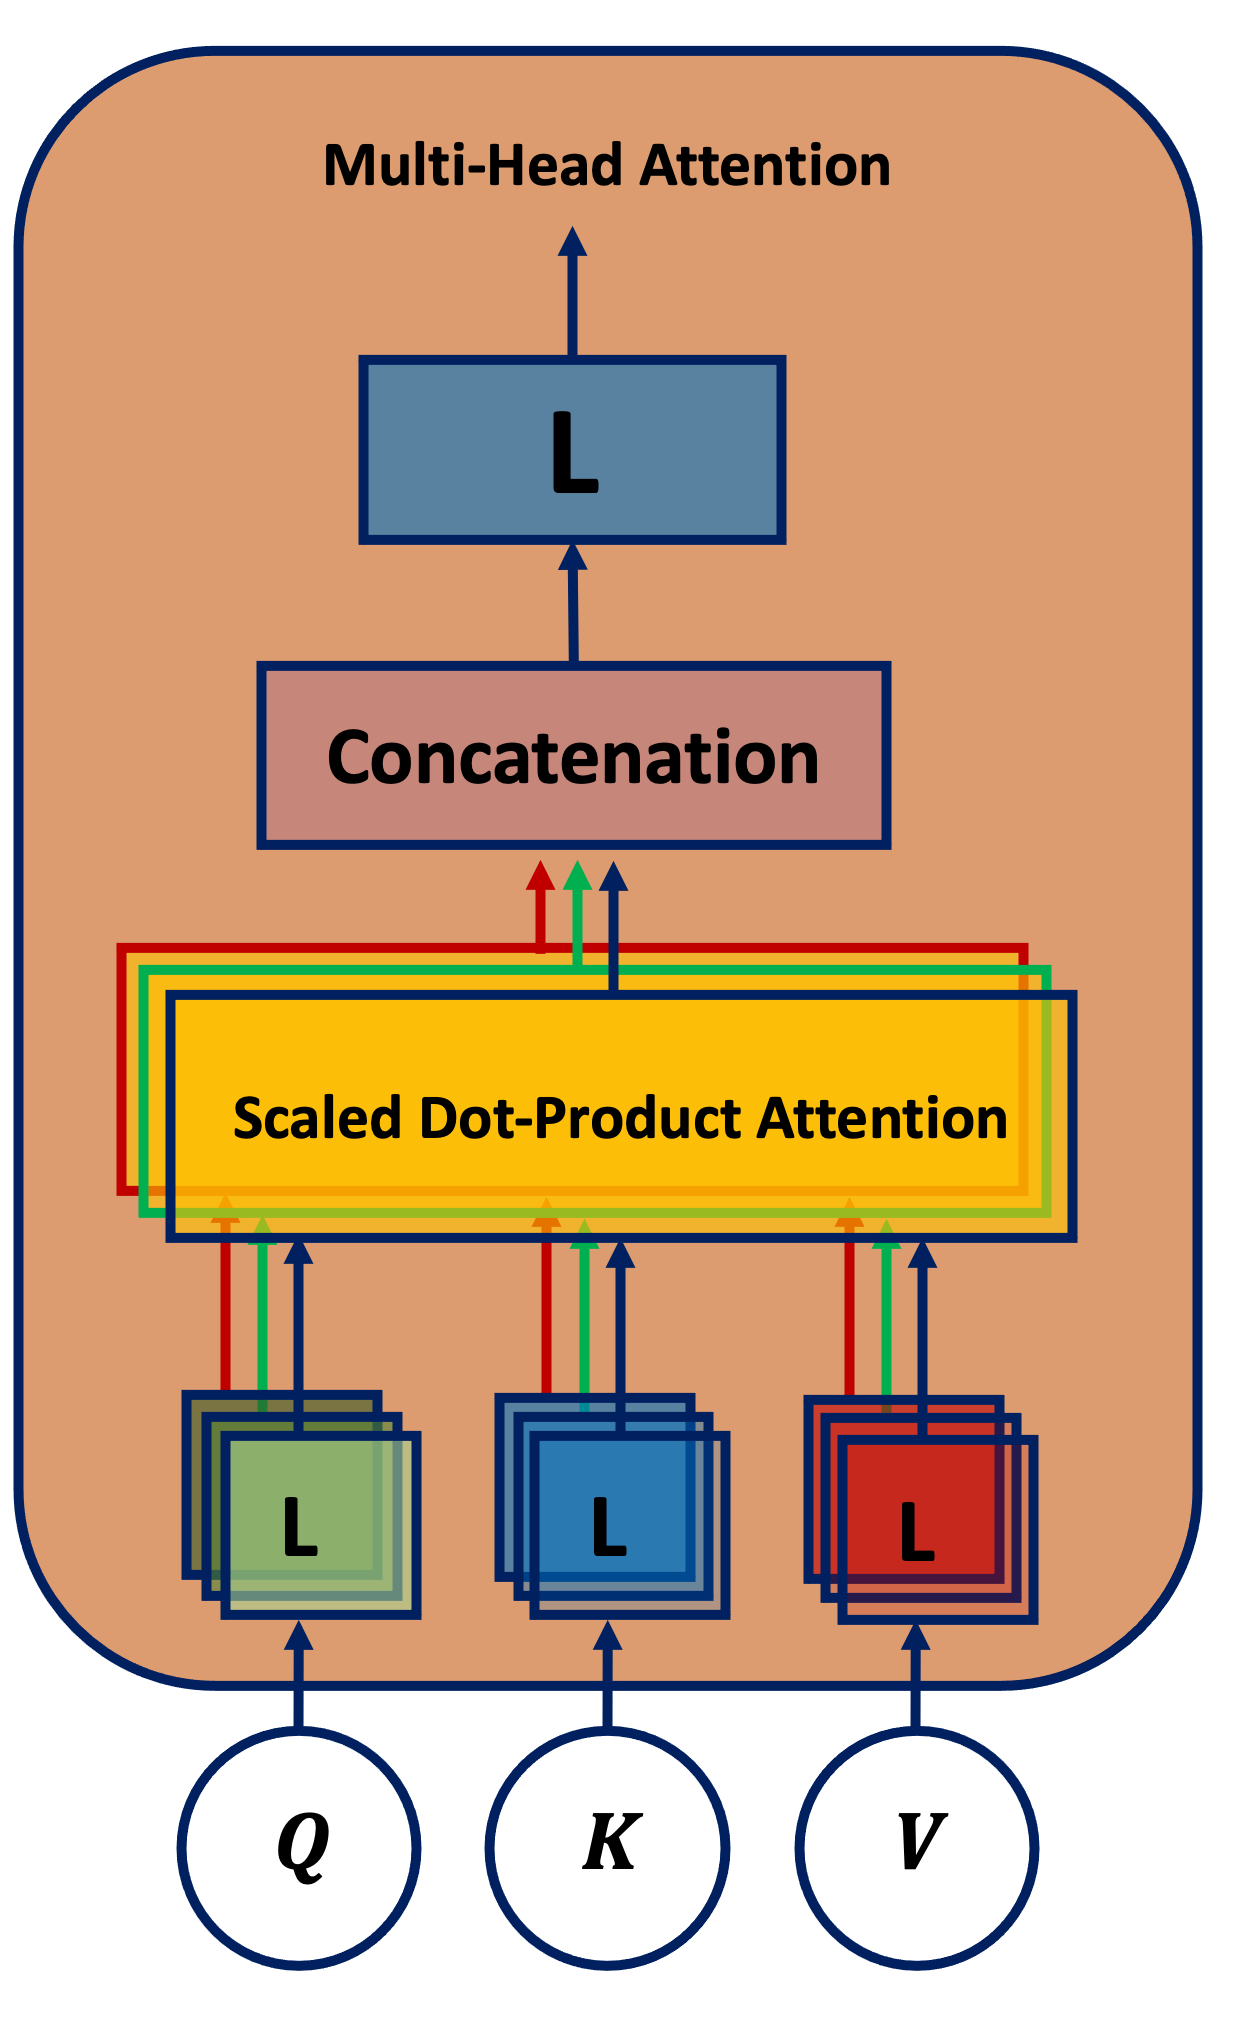
\includegraphics[scale=0.65]{Images/ML/multiHeadAtt.png}
        \caption{Multi-head attention module, where $L$ stands for a linear transformation of the input.} 
        \label{fig:mulitheadAtt}
    \end{subfigure}
    \caption{Multi-head attention mechanism in a transformer. The core operation is an optionally masked scalled dot-product of the queries $Q$, keys $K$, and values $V$. A head consists in three (optionally different) linear projection of the tuple $(Q, K, V)$, each leading to a separate scaled dot-product. The multi-head modules then concatenates all the different head results and finishes with another linear transformation.}
    \label{fig:transAtt}
\end{figure} 

\textbf{Pros:}
\begin{itemize}
    \item \textit{Parallelisation:} The architecture allows for efficient parallelisation of training, speeding up the learning process.
    \item \textit{Capturing Dependencies:} The self-attention mechanism enables the model to capture long-range dependencies in sequences.
    \item \textit{Versatility:} The Transformer architecture has been successfully applied to various \gls{nlp} tasks - including machine translation, text summarization, and language modeling - and computer vision tasks.
\end{itemize}

\textbf{Cons:}
\begin{itemize}
    \item \textit{Computational Complexity:} Training large Transformer models can be computationally expensive, requiring powerful hardware.
    \item \textit{Interpretability:} The attention mechanism, while effective, can be challenging to interpret, making the model somewhat of a "black box."
    \item \textit{Data Dependency:} Transformer models may require large amounts of data for effective training, which may limit their application in domains with limited labeled data.
\end{itemize}

\section{Training and Optimising Deep Learning Models}
Training and optimising neural network models involve a combination of selecting appropriate architectures, fine-tuning hyperparameters - which cannot be learnt by backpropagation-, and employing acceleration techniques to improve efficiency and convergence. In this section, key aspects of the training process are explored, and acceleration techniques commonly used in practice are discussed. \\

\subsection{Training Algorithms}
When optimising the learnable parameters of a model, different strategies can be deployed to update the weights. All mechanisms are refinement on the base gradient descent rule of Equation \ref{eq:gradientdescent}, and each method derived has different \textit{pros and cons}. The two main approaches are: 
\begin{itemize}
    \item \gls{sgd}: the update rule is the same as that of Equation \ref{eq:gradientdescent}, with the only difference being in how the gradient of the weights is computed. Instead of deriving it for the whole dataset (full-batch), the expectation over a random sub-batch is taken, hence the stochastic behaviour: \[ \nabla w = \frac{1}{b} \sum_{s=1}^b \nabla w_s.\] A common observation is that for sub-batches - from now-on referred to as just \textit{batch} - of sufficient size, the stasticial estimator of the gradient based on the batch is unbiased. This greatly accelerates the time it takes to compute the gradient and naturally splits the loop over the dataset into different iterations called \textit{steps}, at which a batch is passed throught the network, a benefitial features in the cases of large datasets that would not fit in memory. 
    \item Adam \cite{adamPaper:} Adam is an algorithm published in 2014 leveraging an adaptive moment estimation approach. The moment in this sense is analoguous to the physical moment and encapsulates the dynamic of the optimisation as stated by the gradient. The idea is that, for larger gradients, the slope is steep and can be quickly traversed, so that any slowing down due to a changing curvature of the objective function landscape could have a mitigated effect on the speed thanks to the inertia of the momentum. This is implemented as an exponentially decaying moving average: the moment $m^t_w$ of weight $w$ at step $t$ is updated with a factor $\beta_1 \in [0, 1[$ such that: \[ m_t \leftarrow \beta_1 m^{t-1}_w + (1 - \beta_1) \nabla_w \mathcal{L}^t,\] where the previous contribution are successively mutliplied by the gradient forgetting factor $\beta_1$. Additionally, another element is taken into account in the gradient descent rule: the second moment $(\nabla_w \mathcal{L}^t)^2$. This tracks how steep the gradient is and, by multiplying the gradient update by a term inversely proportional to the second moment, accelerates the gradient updates in ``flatter'' regions of the objective landscape with the term: \[ v_t \leftarrow \beta_2 v^{t-1}_w + (1 - \beta_2) (\nabla_w \mathcal{L^t})^2.\] To avoiding biasing the gradient update, both the momentum (first moment) and the second moment are corrected with \[\hat{m}^t_w \leftarrow \frac{m^t_w}{1 - \beta_1},\] and \[\hat{v}^t_w \leftarrow \frac{v^t_w}{1 - \beta_2}.\] The two contributions are then combined into a single gradient descent step following equation \ref{eq:adam:}
    \begin{equation}\label{eq:adam}
        w^{t} \leftarrow w^{t-1} - lr \times \frac{\hat{m}^t_w}{\sqrt{\hat{v}^t_w} + \epsilon},
    \end{equation}
    where $\epsilon$ is added for numerical stability.
\end{itemize}

A key hyperparameter in the any gradient descent algorithm is the learning rate $lr$. There is no evident choice for this parameter and the most suitable values are very much derived on a case-by-case approach. A useful technique to let the training process converge to a good minimum of the loss function and avoid unsuitable local minima is to adapt a \textit{learning rate schedule:} the learning rate is modified throughout training to resolve different part of the loss function. Initially, having a relatively larger $lr$ allows the model to quickly update its weights in the direction of the minimum. If the rate is kept to high, the weights will not be able to approach the minimum and will ``bounce' around the target. In order to correct this, the scheduler reduces the $lr$ so that smaller steps can be taken later in the training to approach the chosen optimum. At the beginning, the rate is typically not set to its maximum to start the gradient process in a valley of interest. An equivalent change is to modify the batch size while keeping the $lr$ fixed \cite{smith2017decay}. This has a regularising effect on the gradient: small batch sizes capture large variances and let the optimisation make drastic changes of orientation in the optimising function landscape, thereby avoid unsatisfactory local minima. Larger batch sizes regularise the direction of descent, thereby offering a lower variance but potentially biased estimates towards a minimum. Some method, such as Adam, have specific hyperparameters that should also be optimised with the procedure described later in this chapter.

\subsection{Regularisation}
Regularisation techniques are applied in the architecture and training procudure to prevent overfitting. Common methods include \textit{dropout}, which randomly drops connexions during training with Bernouilli probability distribution of parameter $p$, and L2 (L1) regularisation, which penalises large weights proportionaly to a penalisation parameter $\lambda$ times the sum of the squared (absolute value) of the weights. Both $p$ and $\lambda$ require careful optimisation as regularising the model can introduce bias and limit the overall performance. Batch normalisation is a technique that normalises the inputs of a layer over the batch, reducing internal covariate shift. It helps stabilise and accelerate the training process. This is distinct from the layer normalisation used in the Transformer architecture of section \ref{sec:transformer} as the normalisation is carried over the batch samples rather than the activation. 

\subsection{Hyperparameters Optimisation}
There are several characteristics of the network that need to be optimised. Mainly: 
\begin{itemize}
    \item \textbf{Architecture Selection:} choosing the right architecture is crucial for the success of a \gls{nn}. Factors to consider include the complexity of the task, the nature of the data, and the desired trade-off between model complexity and interpretability. Limits in computing power should be factored in. Elements of the architecture include the type of \gls{ml} chosen (\gls{bdt}, \gls{dnn}, \gls{cnn}, \gls{rnn}, Transformer, ...), the choice of activation functions (\gls{relu}, tanh, ...), and the number of layers and nodes.
    \item \textbf{Hyperparameter Tuning:} optimising hyperparameters - parameters that cannot be optimising through backpropagation of the gradients of the loss - is essential for achieving good model performance. Key hyperparameters include learning rate parameters, batch size, and regularisation parameters.
\end{itemize}
The optimisation process for both hyperparameter tuning and architecture selection is expensive: it requires training and testing models with different combinations of hyperparameters or model architecture to uncover the best peforming options. Techniques such as grid search, random search, and Bayesian optimisation can be employed to efficiently explore the hyperparameter space. Architecture search is usually performed by trials and attempts, and the literature offers insights and guidance into what models might best perform in specific situations. 

\subsection{Acceleration Techniques}
Training an \gls{ml} model is often a computationally demanding tasks that should be carried out more effectively on specifically designed hardware and with some tricks in the process. 
\begin{itemize}
    \item \textbf{Parallel Data Loading:} loading data in parallel can significantly speed up the training process. Libraries like TensorFlow and PyTorch provide functionalities for efficient parallel data loading. Instead of preparing a single batch, multiple batches can be loaded by different processing units to avoid this step becoming a bottleneck in performance. 
    \item \textbf{Early Stopping:} to prevent overfitting and save computation time, early stopping involves monitoring the model's performance on a validation set and halting training when performance ceases to improve.
    \item  \textbf{Hardware Accelerators:} specialised hardware accelerators can further accelerate training. The \gls{gpu} architecture is design to perform simple mathematical operation in parallel. This is precisely the needs of \gls{nn} optimisation, as each step consist in a matrix multiplication. Utilising \gls{gpu} for training and inference can lead to substantial speedup compared to \gls{cpu}-based training. Other types of hardware optimised for \gls{dl} include the Tensor Processing Units (TPU) and the Neural Processing Units (NPU). 
    \item \textbf{Transfer Learning:} transfer learning leverages pre-trained models on large datasets. Fine-tuning these models on specific tasks can significantly reduce the required training time and data. This is becoming increasingly fashionable, as larger \textit{foundational} models trained on multiple tasks with large datasets can then be applied to a specific task, with the pre-trained weights either kept fixed or let free to be modified to optimise the new task. New modules can also be added on top the foundational model to specialise it to a specific use-case. Such large foundational models are already available in \gls{nlp} (e.g., the Mistral 7B \cite{jiang2023mistral} - a 7 billion parameters transformer capable of analysing English sentences and code) and computer vision (for example, the Florence-2 model by Microsoft \cite{xiao2023florence2} - built on a Transformer).
\end{itemize}
Training and optimizing neural network models involve a combination of careful architectural choices, hyperparameter tuning, and the use of acceleration techniques. The selection of appropriate techniques depends on the specific requirements of the task, available resources, and the desired trade-offs between training time and model performance.
